\begin{refsection}
	\startcontents[chapters]	
\chapter{Supervised learning principles and methods}\label{ch:statistical-learning}
%\minitoc
	\printcontents[chapters]{}{1}{}
\section{The supervised learning problem}
\begin{mdframed}
	\textbf{Notation}\cite[12]{mohri2012foundations}
	\begin{itemize}
		\item $\cX$: input space, the set of all possible examples or instances. An instance or an example is usually represented by a feature vector $x = (x_1,...,x_n) \in \cX = \R^n$
		\item $\cY$: the set of all possible labels or target values. For example $\cY=\{-1,1\}$ in binary classification.
		\item $\cD$: the distribution of examples defined on $\cX$ that are used to draw samples.
		\item $D$: a training data set $D = \{(x^{(1)}, y^{(1)}), (x^{(1)}, y^{(1)}), ..., (x^{(n)}, y^{(n)})\}$ drawn from $\cD$.
		\item $\cH$: hypothesis space or hypothesis set
	\end{itemize}
\end{mdframed}

\subsection{Definitions and concepts}




Consider the problem of predicting house prices given a set of characteristics of the house like year built, type, parking, area, utilities. In supervised learning, we are presented with examples of house prices and their characteristics, and our goal is to seek an optimal function or mapping $f(x)$ that captures the relationship between house characteristics and their prices.

Separately, in a loan lending problem, we need to predict a customer's default behavior, in terms of default probability, based on the customer's characteristics such as credit score, age, occupation, etc.




We assume the training data set $D$ consists of IDD samples given by
$$D = \{(x^{(1)}, y^{(1)}), (x^{(1)}, y^{(1)}), ..., (x^{(n)}, y^{(n)})\}$$

\begin{definition}[hypothesis,hypothesis space]\index{hypothesis}\index{hypothesis space}\hfill
	\begin{itemize}
		\item A \textbf{hypothesis} $h$ is a mapping from $\cX$ to $\cY$.
		\item The set of all hypothesis in a learning task form the \textbf{hypothesis space} $\cH$. $\cH$ is usually represented by a family of functions parameterized by some parameters $\theta$.
	\end{itemize}	
	
\end{definition}



\begin{example}[hypothesis space of linear functions]
	Consider a hypothesis space $\cH$ consisting of all linear functions with respect to the input $x\in \R^n$. $\cH$ can be parameterized by
	$$\cH = \{f(x;\theta) = w^Tx + b| w\in \R^n, b\in \R\}.$$	
\end{example}




The two most common supervised learning tasks are \textbf{classification} and \textbf{regression}:
 
\begin{itemize}
	\item \textbf{Classification}: In classification tasks, our goal is to learn a mapping $y = f(x)$ from input $x$ to output $y \in \{1, 2, ..., C\}$, which encodes categories. In some variant of classification, we are learning a probability distribution over categories given $x$, in this case, $f(x) = Pr(y|x)$.
	
	When $C = 2$, the classification is called \textbf{binary classification}; when $C > 2$, the classification is called \textbf{multi-label classification}. 
	\item \textbf{Regression}: In regression tasks, the computer program is asked to predict a
	numerical value given some input. To solve this task, the learning algorithm
	is asked to output a function f : Rn → R. This type of task is similar to
	classification, except that the format of output is different. An example of
	a regression task is the prediction of the expected claim amount that an
	insured person will make (used to set insurance premiums), or the prediction
	of future prices of securities. These kinds of predictions are also used for
	algorithmic trading.
	
\end{itemize}

The input $x$ can take a wide variety of forms, include nominal, ordinal, binary, count, time, or interval, categorical, integer, continuous number, image, video, time series, audio, text, etc. For example 
\begin{figure}[H]
	\centering
	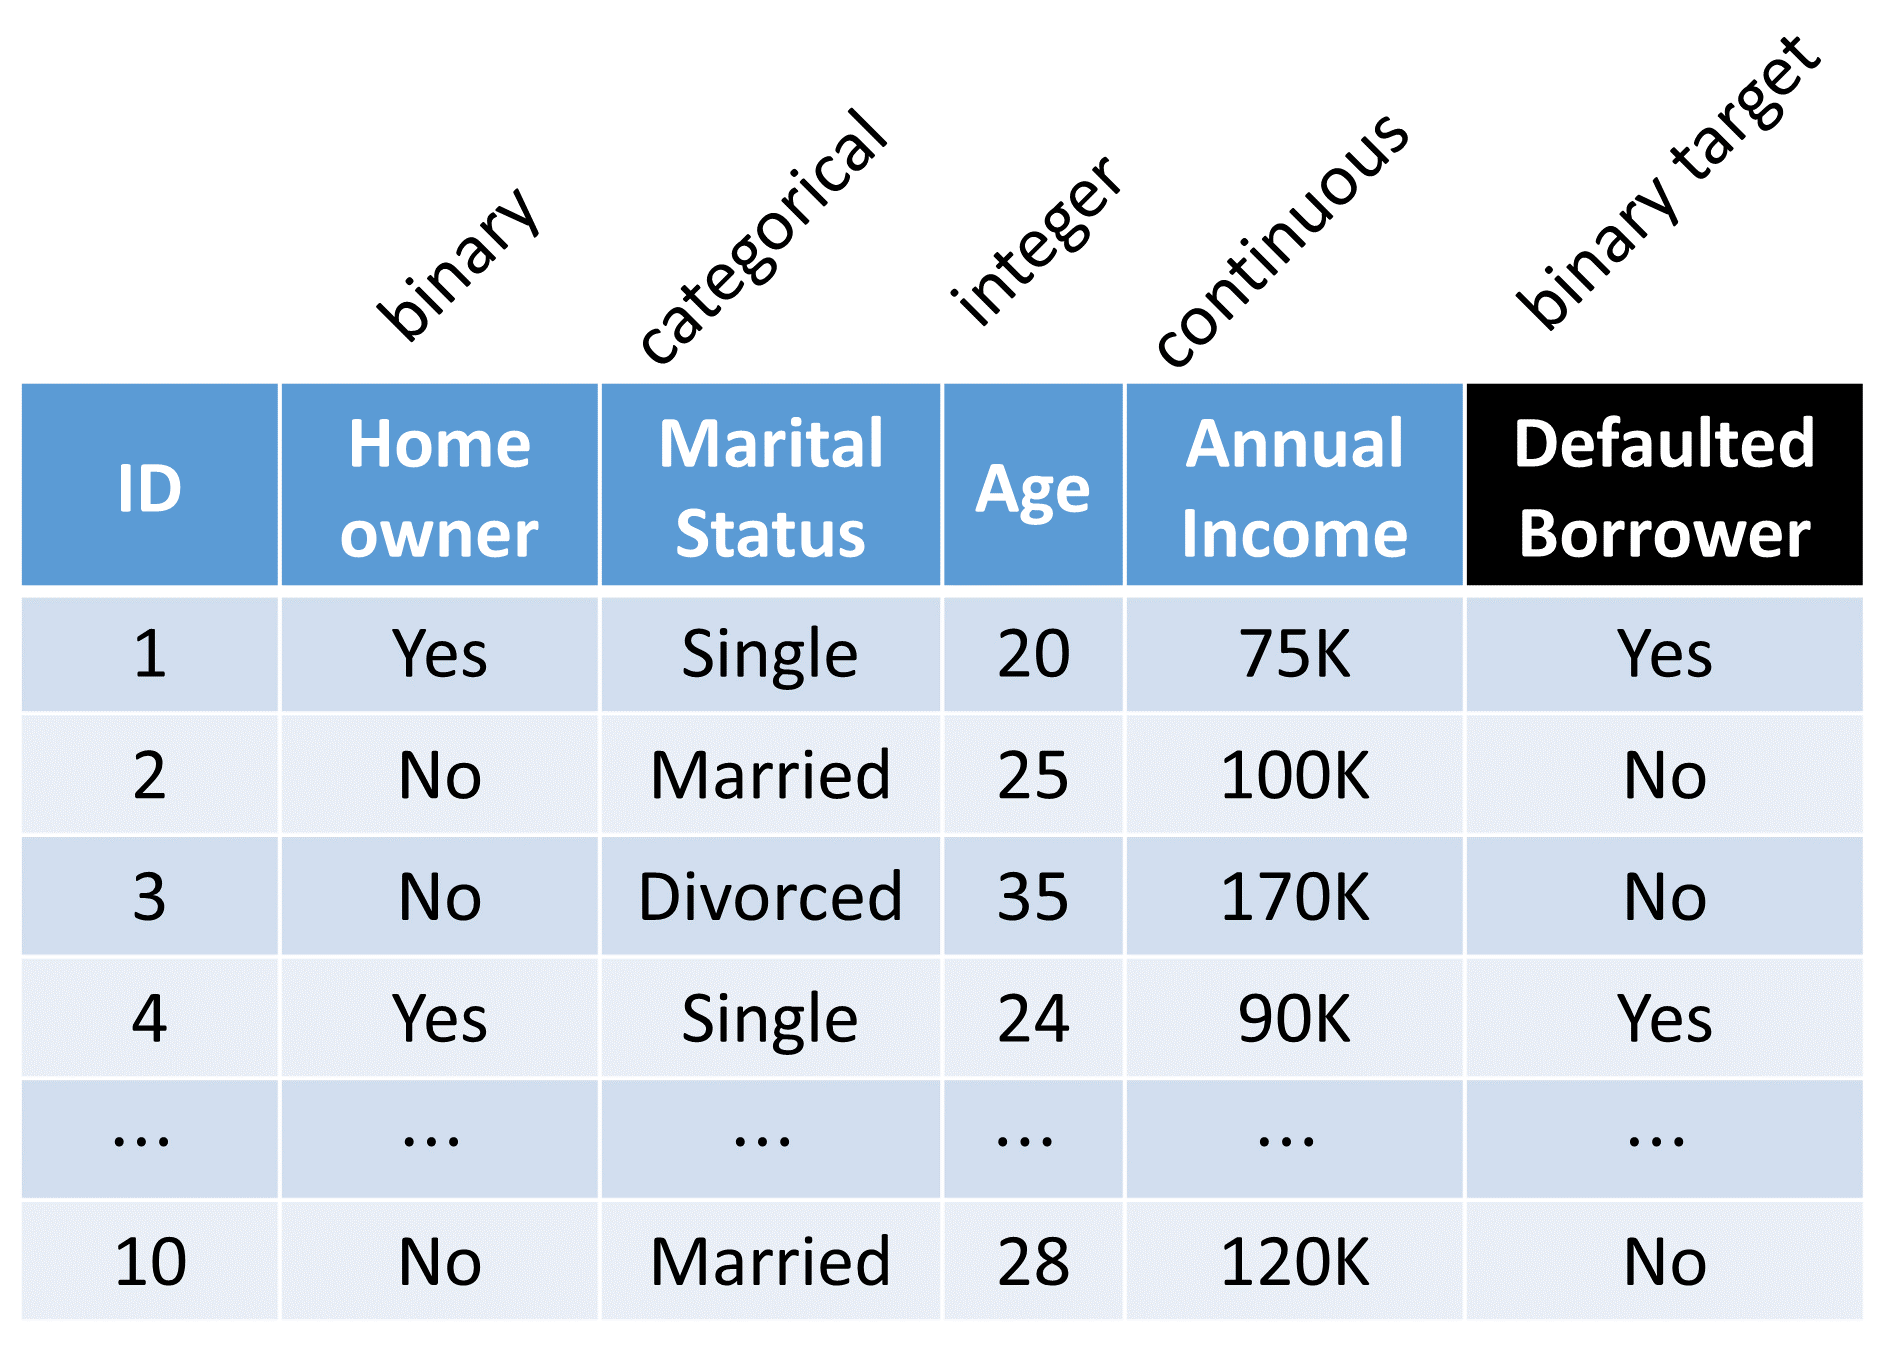
\includegraphics[width=0.5\linewidth]{../figures/statisticalLearning/supervisedLearningPrinciples/SupervisedLearningClassificationDataTypeExample}
	\caption{Input data type examples.}
	\label{fig:SupervisedLearningClassificationDataTypeExample}
\end{figure}



\begin{definition}[generalization error/risk, true error]\index{generalization error}
Given a hypothesis $h\in H$, a target concept $c\in C$, and an underlying distribution $D$, the generalization error or generalization risk of $h$ is defined by
$$R(h) = Pr_{x\sin \cD}[h(x)\neq c(x)] = E_{x\sin \cD}[1_{h(x)\neq c(x)}]$$
where $1_w$ is the indicator function of event $w$.
\end{definition}


\begin{definition}[empirical error/risk,training error ]\index{empirical error}\index{training error}
Given a hypothesis $h\in H$, a target concept $c\in C$, and an underlying distribution $D$, a set $S$ of training sample pairs $\{(x_i,c(x_i))\}$, the generalization error or generalization risk of $h$ is defined by
$$\hat{R}(h) = \sum_{i=1}^m 1_{h(x_i)\neq c(x_i)}/m$$
where $1_w$ is the indicator function of event $w$.
\end{definition}

\begin{remark}
The \textbf{true error} of a hypothesis $h$ is the probability that it will misclassify a single randomly drawn instance from the distribution $\mathcal{D}$.
\end{remark}

\begin{lemma}[empirical error vs true error]
Consider a hypothesis $h$, we have
$$E[\hat{R}(h)] = R(h)$$
that is empirical error is the unbiased estimator of true error.
\end{lemma}
Proof: use linearity of expectation.


\begin{mdframed}
\textbf{\large The learning problem}\cite[12]{mohri2012foundations}\\

The learner is given a set $S$ of sample pairs $\{x_i,c(x_i)\}, c\in C$ drawn from an unknown distribution $\cD$. His task is to find a hypothesis $h$ in $\cH$ such that the generalization error/true error is minimized.
\end{mdframed}

\begin{remark}
Note that the goal for the learner is to minimize \textbf{true error instead of empirical error}. However, because usually $c$ and $\cD$ is unknown to the learner, the true error cannot be calculated from training sample. 
\end{remark}


\subsection{Function approximation as machine learning task}
Problem setting:
\begin{itemize}
	\item Set of possible instance $X$
	\item Unknown target function $f:X\rightarrow Y$
	\item Set of function hypotheses $H=\{h|h:X\rightarrow Y\}$
\end{itemize}

Input:
\begin{itemize}
	\item Training examples $\{<x^{(i)},y^{(i)}>\}$ of unknown target function $f$
\end{itemize}

Output:
\begin{itemize}
	\item Hypothesis $h\in H$ that best approximates target function $f$
\end{itemize}



\subsection{Overfitting}
Consider error of hypothesis $h$ over
\begin{itemize}
    \item training data
    \item entire distribution $\mathcal{D}$ of data, or simply the input $X$ has a distribution of $\mathcal{D}$
\end{itemize}
Hypothesis $h\in H$ over-fits training data if there is an alternative hypothesis $h'\in H$ such that
$$error_{train}(h) < error_{train}(h')$$
and
$$error_{\mathcal{D}}(h) > error_{\mathcal{D}}(h')$$




\subsection{True error vs. training error}
The \textbf{sample error}, $error_S(h)$ of hypothesis $h$ with respect to target function $f$ and data sample $S$ is given as:
$$error_S(h)=\frac{1}{n}\sum_{x\in S}\delta(f(x),h(x))$$
where $n$ is the number of examples in $S$.\\
 mathematically, we have
$$error_D(h) = Pr_{x \in \mathcal{D}}(f(x)\neq h(x))$$
where $Pr_{x \in \mathcal{D}}$ denotes that the probability is taken over the instance distribution $\mathcal{D}$



\subsection{Generative classifier vs. discriminative classifier }\cite{jordan2002discriminative}
\textbf{Generative classifier} learn a model of the joint probability, $p(x,y)$, of the inputs $x$ and the label $y$, and make their prediction using Bayes rules to calculate $p(y|x)$, then picking the most likely label $y$.\\
\textbf{Discriminative classifiers} model the posterior $p(y|x)$ directly, or learn a direct map from inputs $x$ to the class labels $y$, which avoid the intermediate step in generative classifiers. 

\subsection{No free lunch theorem}


\begin{align*} 
\sum_{f} E_{o t e}\left(\mathfrak{L}_{a} | X, f\right) &=\sum_{f} \sum_{h} \sum_{x \in \mathcal{X}-X} P(\boldsymbol{x}) \mathbb{I}(h(\boldsymbol{x}) \neq f(\boldsymbol{x})) P\left(h | X, \boldsymbol{\Sigma}_{a}\right) \\ &=\sum_{\boldsymbol{x} \in \mathcal{X}-X} P(\boldsymbol{x}) \sum_{h} P\left(h | X, \boldsymbol{\Sigma}_{a}\right) \sum_{f} \mathbb{I}(h(\boldsymbol{x}) \neq f(\boldsymbol{x})) \\ &=\sum_{x \in \mathcal{X}-X} P(\boldsymbol{x}) \sum_{h} P\left(h | X, \mathcal{L}_{a}\right) \frac{1}{2} 2^{|\mathcal{X}|} \\ &=\frac{1}{2} 2^{|\mathcal{X}|} \sum_{\boldsymbol{x} \in \mathcal{X}-X} P(\boldsymbol{x}) \sum_{h} P\left(h | X, \boldsymbol{\Sigma}_{a}\right) \\
&=2^{|\mathcal{X}|-1} \sum_{\boldsymbol{x} \in \mathcal{X}-X} P(\boldsymbol{x}) \cdot 1
\end{align*}



\section{Variance bias trade-off}

\subsection{Overfitting and underfitting phenomenon}

\begin{figure}
	\centering
	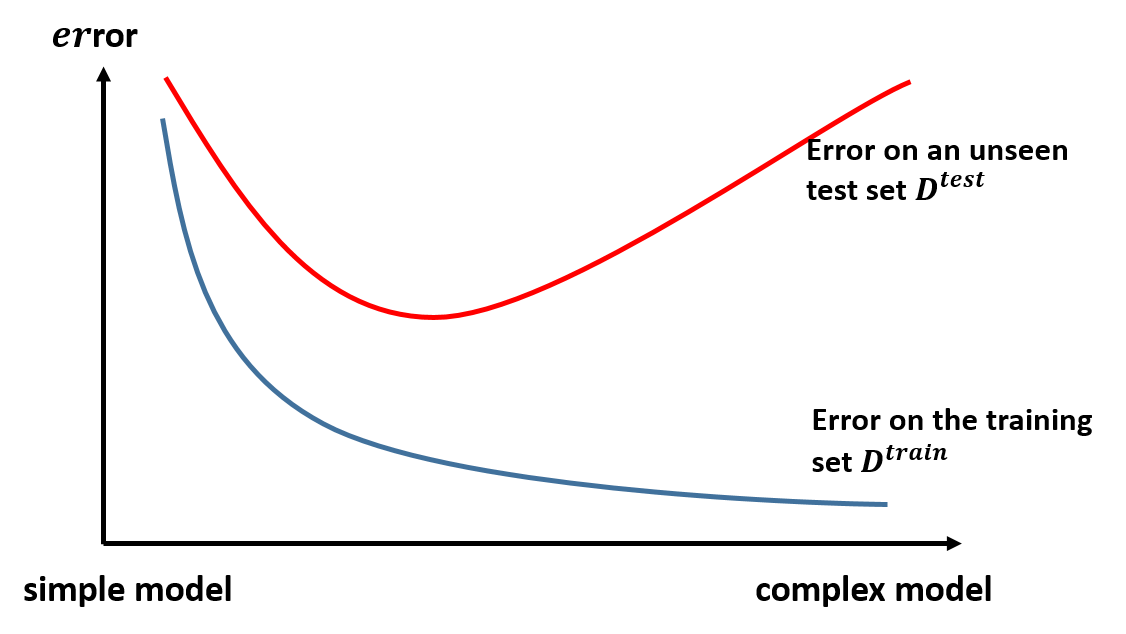
\includegraphics[width=0.6\linewidth]{../figures/statisticalLearning/supervisedLearningPrinciples/underFittingOverfittingDemo}
	\caption{The commonly observed phenomenon of overfitting and underfitting in machine learning. }
	\label{fig:underfittingoverfittingdemo}
\end{figure}





\subsection{Fundamentals}

\begin{lemma}[variance-bias tradeoff]\cite[34]{james2013introduction}
Suppose our training examples $(x,y)$ are generated via
$$y = h(x) + \epsilon$$
where $\epsilon$ is \textbf{an independent random variable with zero mean}. Let $\hat{f}$ be our proposed model with model parameters needs to be estimated from training examples $\cD$. Let us measure our learning performance via $E_\cD[(y_0 - \hat{f}(x_0|\cD))^2]$, that is the mean square error between the trained model and the real model \textbf{when given training examples with a finite number $N$.}
$$E_{\cD}[(y_0 - \hat{f}(x_0))^2] = Var_\cD[\hat{f}(x_0|\cD)] + [Bias(\hat{f}(x_0|\cD))]^2 + Var[\epsilon]$$
where
$Bias(\hat{f}(x_0|\cD)) = E[\hat{f}(x_0|\cD) - f(x)]$, $(x_0,y_0)$ is a training example drawn randomly from the population, and all the expectations are respect to the population distribution $\cD$.
\end{lemma}
\begin{proof}
(1)Use the following decomposition:
\begin{align*}
 &E_{\cD}[(y - \hat{f}(x|\cD))^2] \\
=&E_\cD[(y - h(x) + h(x) - \hat{f}(x|\cD))^2] \\
=&E_\cD[(y - h(x))^2] + 2E_\cD[(h(x) - \hat{f}(x|\cD))(y - h(x))] + E_\cD[(h(x) - \hat{f}(x|\cD))^2] \\
=&E_\cD[(y - h(x))^2] + 2E_\cD[(h(x) - \hat{f}(x|\cD))\epsilon] + E_\cD[(h(x) - \hat{f}(x|\cD))^2] \\
=&\underbrace{E_\cD[(y - h(x))^2]}_{noise~term}+ 0 + \underbrace{E_\cD[(h(x) - \hat{f}(x|\cD))^2]}_{model~estimation~error}. 
\end{align*}
where the noise term is without our control and the model estimation error is what we want to minimize.
(2)

\end{proof}



\begin{remark}[interpretation of Variance term]\hfill
\begin{itemize}
	\item $Var[\hat{f}(x_0)]$ represents the amount by which $\hat{f}$ would change if we estimate the model parameter using a different set of training examples of fixed size $n$. 
	\item If this term is large, then we are likely to have large test error.
	\item When increasing the number training examples, this term will be reduced. 
	\item Given a fixed number of training examples, a more flexible model(model with more parameters) will tend to have large variance since each parameter will be estimated poorly.
\end{itemize}
\end{remark}

\begin{remark}[interpretation of Bias term]\hfill
	\begin{itemize}
		\item $E[\hat{f}]$ is the resulting trained model when given infinitely number of training examples. Therefore, $(E[\hat{f}] - f)^2$ reflect the fundamental error associated with model proposal/assumption. For example, if $f$ is nonlinear model and $\hat{f}$ is a linear model, then no matter how hard we train, we cannot eliminate this error. 
		\item A less flexible model(such as linear model) will tend to have large bias. When using "universal approximation" models, like neural network and decision tree, the bias term could be reduced, however, at the risk of increasing Variance term.
	\end{itemize}
\end{remark}


\begin{remark}[interpretation of noise term]\hfill
	\begin{itemize}
		\item Even we have perfect model, that is $Bias[\hat{f}] = 0$, and perfect estimation of the model $Var[\hat{f}]=0$, we will cannot reduce 
		$E[(y_0 - \hat{f}(x_0))^2]$ to zero because the $y_0$ always contains a noise that cannot be predicted.
	\end{itemize}
\end{remark}

\begin{method}[estimating error]
Fix the test example $(x_0,y_0)$, we can do the following experiment:
\begin{itemize}
	\item Draw a training examples $D_1$ of size $N$, $D_1=\{(x_1,y_1),(x_2,y_2),...,(x_N, y_N)\}$.
	\item Train linear regression $\hat{f}(x|D_1)$ using $D_1$.
	\item Calculate the squared error
	$$err(D_1) = (\hat{f}(x_0|D_i) - y_0)^2.$$
	\item Repeat the above procedures by drawing different training examples $D_i,i=2,...,M$, and get the mean squared error via
	$$err = \frac{1}{M}\sum_{i=1}^M err(D_i).$$ 
\end{itemize}	
\end{method}

\subsection{Examples}

\subsubsection{Linear regression}
\begin{lemma}
Assume the true model is $h(x) = x^T\beta$ and the prediction model is $$\hat{f}(x|\cD) = x^T\hat{\beta},$$
where $\hat{\beta} = (X^TX)^{-1}X^TY$.
It follows that
\begin{itemize}
	\item Unbiasedness:
	$$E_\cD[\hat{f}(x)|\cD] = h(x) = x^T\beta.$$
	\item Variance:
	$$Var\triangleq E_{\cD}[(\hat{f}(x)|\cD - E_\cD[\hat{f}(x)|\cD])^2] = \sigma^2 x^T(X^TX)^{-1}x.$$
	\item If inputs $X$ are standardized and $x$ is a random vector with distribution $MN(0,I_{p\times p})$, then
	$$Var\approx \sigma^2 \frac{p}{n}.$$
\end{itemize}	
\end{lemma}
\begin{proof}
(1)(2) see \autoref{ch:statistical-models:th:OrdinaryLinearRegressionleastSquareSolution}.
(3)
\begin{align*}
E_{x}[Var] &=  E_{x}[\sigma^2 x^T(X^TX)^{-1}x] \\
&=  \sigma^2E_{x}[Tr( x^T(X^TX)^{-1}x)] \\
&=  \sigma^2E_{x}[Tr( (X^TX)^{-1}xx^T)] \\
&=  \sigma^2 E_{x}[Tr( xx^T(X^TX)^{-1})] \\
&=  \sigma^2 Tr(E_{x}[xx^T] (X^TX)^{-1})\\
&=  \sigma^2 Tr(I_{p\times p} )
\end{align*}
\end{proof}


\subsubsection{K-nearest neighbor}


\section{Model regularization}
\subsection{KL divergence}

\begin{definition}[Kullback-Leibler divergence, KL divergence]\index{KL divergence}
	Given two discrete probability distribution $P$ and $Q$ defined on the same set $\cX$, the KL divergence from $Q$ to $P$ is defined as
	$$D_{KL}(P||Q) = \sum_{x\in\cX} P(x)\log \frac{P(x)}{Q(x)}$$ 
\end{definition}

\begin{lemma}[non-negativeness of KL divergence]\label{ch:statistical-learning:th:KLDivergenceProperty}
	Given two discrete probability distribution $P$ and $Q$ defined on the same set $\cX$,
	$$D_{KL}(P||Q)\geq 0.$$
	And the equality holds if $P=Q$.
\end{lemma}
\begin{proof}
	$$D_{KL}(P||Q) = -\sum_{x\in\cX} P(x)\log \frac{Q(x)}{P(x)}\geq - \log (\sum_{x\in\cX} \frac{Q(x)}{P(x)} P(x)) = 0$$
	where the fact that $-\log(x)$ is a convex function and Jensen's inequality has been used(\autoref{ch:theory-of-probability:th:Jenseninequality}).
\end{proof}




\section{Model evaluation}
\subsection{Loss metrics}

\begin{definition}[loss function for classification]\cite[28]{Qiu2019NeuralLearning}
	\begin{itemize}
		\item 0-1 loss function
		$$L_{0-1}(y, f(x;\theta)) = I(y \neq f(x;\theta)).$$
		\item cross-entropy loss function
		$f_c(x;\theta) = p(y = c|x;\theta)$
		$$\mathcal{L}(\boldsymbol{y}, f(\boldsymbol{x} ; \theta))=-\sum_{c=1}^{C} y_{c} \log f_{c}(\boldsymbol{x} ; \theta)$$
		where $y_c$ is the one-hot encoding of the sample label.
		\item Hinge loss function
		$$\mathcal{L}(y, f(\boldsymbol{x} ; \theta))=\max (0,1-y f(\boldsymbol{x} ; \theta)) = (1 - yf(x;\theta))^+.$$
		
	\end{itemize}
\end{definition}

\begin{example}\hfill
\begin{itemize}
	\item 
	\item For example, consider a 3-class classification problem. Assume one sample has label $y = (1, 0, 0)$, and the prediction gives $f(x;\theta) = (0.5, 0.3, 0.2)$. Then the cross entropy contribution from this example is given by
	$$-(1\times \log (0.5)) - (0 \times \log(0.3)) - (0 \times \log(0.2))$$
	
\end{itemize}


\end{example}


\begin{remark}
\begin{itemize}
	\item Although 0-1 loss function is mathematically simple, it is not differentiable and therefore difficult to optimize.
	\item Cross entropy loss function can also be viewed as the negative log-likelihood function
\end{itemize}
\end{remark}



\begin{definition}[accuracy]\cite[47]{Qiu2019NeuralLearning}
	\begin{itemize}
		\item 
		$$ACC = \frac{1}{N} \sum_{n=1}^{N} I\left(y^{(n)}=\hat{y}^{(n)}\right)$$
		\item 
		$$
		ERR = 1 - ACC = =\frac{1}{N} \sum_{n=1}^{N} I\left(y^{(n)} \neq \hat{y}^{(n)}\right)
		$$
	\end{itemize}
	
	For a specific class label $c$, there are four classification results.
	\begin{itemize}
		\item true positive, TP, where the sample's true label is $c$ and the predicted label is $c$. More formally, we define
		$$TP_{c}=\sum_{n=1}^{N} I\left(y^{(n)}=\hat{y}^{(n)}=c\right).$$		
		\item false positive, FP, where the sample's true label is not $c$ but the predicted label is $c$. More formally, we define
		$$FP_{c}=\sum_{n=1}^{N} I\left(y^{(n)} \neq c \wedge \hat{y}^{(n)}=c\right)$$
		
		\item true negative, TN, where the sample's true label is not $c$ and the predicted label is not $c$.
		$$TN_{c}=\sum_{n=1}^{N} I\left(y^{(n)}\neq c \wedge \hat{y}^{(n)} \neq c\right)$$
		
		
		\item false negative, FN, where the sample's true label is $c$ and the predicted label is not $c$. More formally, we define
		$$FN_{c}=\sum_{n=1}^{N} I\left(y^{(n)}=c \wedge \hat{y}^{(n)} \neq c\right)$$
		
		
	\end{itemize}
	
	
\end{definition}


\begin{definition}
	\begin{itemize}
		\item precision is the ratio of the number of correct prediction over the number of total prediction on label $c$: 
		$$P_c =\frac{T P_{c}}{T P_{c}+F P_{c}}$$
		\item recall is 
		$$R_{c}=\frac{T P_{c}}{T P_{c}+F N_{c}}$$
		\item $F$ measure
		$$\mathcal{F}_{c}=\frac{\left(1+\beta^{2}\right) \times P_{c} \times R_{c}}{\beta^{2} \times P_{c}+R_{c}}$$
		where $\beta$ is the parameter to adjust the relative importance of precision and recall
		Usually, $\beta = 1$, and in this case, $F$ measure to denoted by $F_1$.
		
		
		
	\end{itemize}
	
	\begin{itemize}
		\item Macro Average is the ratio of the number of correct prediction over the number of total prediction on label $c$: 
		\begin{align*}
		P_{marcro} &=\frac{1}{K} \sum_{c=1}^K P_c \\
		R_{marcro} &=\frac{1}{K} \sum_{c=1}^K P_c \\
		F_{1,marcro} &=\frac{1}{K} \sum_{c=1}^K P_c 
		\end{align*}
		
		\begin{align*}
		P_{marcro} &=\frac{1}{K} \sum_{c=1}^K P_c \\
		R_{marcro} &=\frac{1}{K} \sum_{c=1}^K P_c \\
		F_{1,marcro} &=\frac{1}{K} \sum_{c=1}^K P_c 
		\end{align*}
		
		
		
		
		\item recall is 
		$$R_{c}=\frac{T P_{c}}{T P_{c}+F N_{c}}$$
		\item $F$ measure
		$$\mathcal{F}_{c}=\frac{\left(1+\beta^{2}\right) \times P_{c} \times R_{c}}{\beta^{2} \times P_{c}+R_{c}}$$
		where $\beta$ is the parameter to adjust the relative importance of precision and recall
		Usually, $\beta = 1$, and in this case, $F$ measure to denoted by $F_1$.
		
		
		
	\end{itemize}
	
	
	
\end{definition}




\subsection{Regression metric}

\begin{definition}
Denote $\hat{y}$ as the estimated target output, $y$ the corresponding (correct) target output, $\hat{y}_i$  the predicted value of the $i$-th sample, and $y_i$ the corresponding true value
\begin{itemize}
	\item (explained variance) The \textbf{explained variance} is estimated as follow:	
	$$explained_variance(y,\hat{y}) = 1 - \frac{Var[y-\hat{y}]}{Var[y]}.$$
	\item (mean absolute error)the mean absolute error (MAE) estimated over $N$ samples is defined as	
	$$MAE(y,\hat{y}) = \frac{1}{N}\sum_{i=1}^{N} \abs{y_i - \hat{y}_i}.$$
	\item (mean squared error) If $\hat{y}_i$ is the predicted value of the $i$-th sample, and $y_i$ is the corresponding true value, then the mean squared error (MSE) estimated over $N$ samples is defined as	
	$$MSE(y,\hat{y}) = \frac{1}{N}\sum_{i=1}^{N} (y_i - \hat{y}_i)^2.$$
	\item (median absolute error) If $\hat{y}_i$ is the predicted value of the $i$-th sample, and $y_i$ is the corresponding true value, then the mean squared error (MSE) estimated over $N$ samples is defined as	
	$$MadAE(y,\hat{y}) = median(\abs{y_1 - \hat{y}_1},...,\abs{y_N - \hat{y}_N},)^2.$$
\end{itemize}	
\end{definition}

\subsection{Summary}

\begin{itemize}
	\item For a given model, increasing training data will increase training error and decrease testing error. As training data size goes to infinitely large, training error and testing error will converge to the true error.
\end{itemize}


\section{Model selection methods}

\subsection{Basic idea}
To prevent overfitting in supervised learning algorithms, it is common practice to split the data to training set and testing data where the model parameters are estimated based on the training data and the performance evaluation is conducted on the testing data set. 

For a set of models parameterized by hyperparameters (e.g., the regularizer parameter in the penalized linear regression), using performance evaluation on the testing data set to determine the optimal hyperparameters has the risk of  overfitting on the testing data set (i.e., the model might still perform bad for samples never seen before.). This is because the during the hyperparameter searching process, knowledge about the testing data set can 'leak' into the model and evaluation metrics no longer report on generalization performance. To solve this problem, commond practice is to dividend the data set into \textbf{training set, validation set, and testing set}. 
In such way, training proceeds on the training set, after which hyperparametering tuning is done on the validation set. In the end, final evaluation of the model is done on the test set.

\subsection{Cross-validation}

As our previous discussion, training a model with hyperparameters requires the partitioning of the available data into three sets. This procedure has the following drawbacks:
\begin{itemize}
	\item The number of samples used for training will be draticaly reduced.
	\item The result will be that the results can depend on a particular choice for the pair of (train, validation) sets.
\end{itemize} 

One solution to these issues is a procedure called \textbf{cross-validation (CV)}. 
\begin{method}[$K$-fold CV procedure]
\begin{itemize}
	 \item training set is split into k smaller sets (other approaches are described below, but generally follow the same principles). The following procedure is followed for each of the k “folds”.
	 \item A model is trained using k-1 of the folds as training data;
	 \item the resulting model is validated on the remaining part of the data (i.e., it is used as a test set to compute a performance measure such as accuracy).
	 \item The performance measure reported by k-fold cross-validation is then the average of the values computed in the loop.
\end{itemize}	
\end{method}


A test set should still be held out for final evaluation, but the validation set is no longer needed when doing CV. In the basic approach, called k-fold CV, the

A model is trained using k-1 of the folds as training data;
the resulting model is validated on the remaining part of the data (i.e., it is used as a test set to compute a performance measure such as accuracy).
 This approach can be computationally expensive, but does not waste too much data (as it is the case when fixing an arbitrary test set), which is a major advantage in problem such as inverse inference where the number of samples is very small.
 
 
\subsection{Statistical comparison}
 



\subsubsection{Occam's razor}
The simplest hypothesis that fits the data is preferred.


\section{Data preprocessing and feature engineering}




\subsection{Handle missing values}


For various reasons, many real world datasets contain missing values, often encoded as blanks, NaNs or other placeholders. Such datasets however are incompatible with most of the machine learning algorithms.  

One basic strategy to handle incomplete data matrix $X$ is to discard entire rows (i.e., discard the example) and/or columns (i.e., discard the feature) containing missing values. However, this comes at the price of losing data which may be valuable (even though incomplete). A better strategy is to impute the missing values, i.e., to infer them from the known part of the data based on some assumed distributions on missing values.

In practice, some ad hoc strategy is to impute missing values using either the mean, the median or the most frequent value of the row or column in which the missing values are located. The code example is in 


\subsection{Data standardization}







\subsection{Handle categorical data}

\href{https://www.analyticsvidhya.com/blog/2015/11/easy-methods-deal-categorical-variables-predictive-modeling/}{link}


\begin{table}[H]
	\begin{tabular}{cccc}
		Categorical Value & $x_1$ & $x_2$ & $x_3$ \\
		Married           & 1     & 0     & 0     \\
		Single            & 0     & 1     & 0     \\
		Divorced          & 0     & 0     & 1    
	\end{tabular}
\end{table}












\section{Kernel methods}
\subsection{Basic concepts of kernels and feature maps}
\begin{mdframed}
	\textbf{\cite[481]{murphy2012machine} General motivations:}
	\begin{itemize}
		\item for some data(such at text document, colloidal structure) it is not easy to represent the data as a vector in $\R^d$
		\item By assuming that we have some way to measure the similarity between different input example, we design algorithms using similarity as input for classification and regression. Such similarity measure is the kernel function.
	\end{itemize}
\end{mdframed}


\begin{definition}[kernel] \index{kernel}
	\cite[90]{mohri2012foundations}A function $K:X\times X \to \F$ is called a kernel over $X$.
\end{definition}


\begin{definition}[feature map, feature, feature space]\index{feature map}\index{feature space}\index{feature}
	In machine learning, a \textbf{feature map} is usually an embedding:
	$$\phi:R^D\to\R^M$$
	with $M \gg D$. The point $\phi(x) \in \R^M$ is called the \textbf{feature} of data point $x\in \R^D$.
	The space $\R^M$ is called the \textbf{feature space}.
\end{definition}

\begin{remark}[relations between kernel and feature map]
	\begin{itemize}\hfill
		\item For general kernels, usually there is no connection between the two.
		\item When the kernel satisfies certain conditions, say Mercer's condition, one can show that the kernel is implicitly associated with a feature map. \textbf{This association is significant, it enables us to use some implicitly complex feature maps to do machine learning tasks by only doing calculation using relatively 'simple' kernels.}
	\end{itemize}
\end{remark}



\begin{example}[\textbf{linear kernel}]
	\cite[484]{murphy2012machine} If the original data is already in $\R^d$, we can use $\phi(x) = x,k(x,x')= x^Tx'$. \textbf{This kernel is useful only when (1) $x$ is high dimensional (2) every individual dimension is informative(providing useful information)}. In the example of image recognition, linear kernel will be a bad choice since not every pixel is informative.  
\end{example}


\begin{remark}
	More complex feature(high-dimensional) space usually enable us to distinguish distributions with different means.
\end{remark}





\subsection{Mercer's theorem}

\begin{definition}[positive definite symmetric kernel]\index{positive definite symmetric kernel}\index{Gram matrix}
	\cite[92]{mohri2012foundations}\cite[30]{scholkopf2002learning}A kernel $k:X^2\to \F$ is said to be positive definite symmetric(PDS) if for any $x_1,x_2,...,x_m \in X$, the matrix $K_{ij} = k(x_i,x_j)$ is symmetric semi-positive definite matrix. The matrix $K$ is called \textbf{Gram matrix} of $k$ with respect to $x_1,x_2,...,x_m$.
\end{definition}

\begin{lemma}[Cauchy-Schwarz inequality for PDS kernel]
	If $k$ is a PDS kernel, then
	$$\abs{k(x_1,x_2)} \leq k(x_1,x_1)k(x_2,x_2)$$
\end{lemma}
Proof: from $det K \geq 0$, where $K$ is the Gram matrix.


\begin{remark}[interpretation]
	In studying approximation theory in vector space using basis functions, we also define Gram matrix with entries being the dot product of basis function. Here, we view the \textbf{input data vectors as the basis of the input vector space}.
\end{remark}


\begin{definition}[Mercer's condition]\index{Mercer's condition}
	A real-valued function $k:X\times X \to \R$ is said to fulfill Mercer's condition if for \textbf{all square integrable functions} $g(x)$ one has
	$$\int_X\int_X g(x)K(x,y)g(x) dxdy \geq 0$$
	Or in discrete case, the $k$ is replaced by a matrix $K\in \R^{N\times N}$, such that for all vectors $g\in \R^N$ such that
	$$\ip{g,Kg} = g^T K g \geq 0$$
\end{definition}


\begin{theorem}[Mercer's theorem]\index{Mercer's theorem}
	\cite{wiki:Mercer}\cite[64]{shawe2004kernel}
	Suppose $k:X\times X\to \R$ is a continuous symmetric non-negative definite kernel, that is, it satisfies Mercer's condition. Then there is an orthonormal basis $e_i(x)$ of $L^2(X)$ such that
	$$k(s,t) = \sum_{j=1}^\infty \lambda_i e_j(s)e_j(t)$$
	where $\lambda_i \geq 0$
\end{theorem}

\begin{remark}[interpretation \& significance]\hfill
	\begin{itemize}
		\item The mercer's theorem enables us to interpret that: for symmetric semi-positive definite kernels, there exist feature maps given as $\phi(x) =\sum_i \sqrt{\lambda_i}e_i(x) $ such that $k(s,t) = \ip{\sum_i \sqrt{\lambda_i}e_i(s),\sum_i \sqrt{\lambda_i}e_i(s)}$
		note that it would be difficult to recover the underlying functions $e_i(x)$ and $\lambda_i$.
		\item The mercer's theorem enables us to connect kernel to feature maps when mercer's condition holds. \textbf{Note that for an arbitrary kernel, the concept of kernel and feature map might be unrelated.} 
	\end{itemize}
\end{remark}



\begin{remark}[the underlying feature map]
	Given a kernel function $k$ satisfying Mercer's condition,\textbf{the feature map and the feature space are implicitly defined}, and it is usually hard to find the underlying feature map $\phi(x)$ is(because of the uniqueness issue for example).
	But if we are given a feature map $\phi(x)$, calculating a 'canonical' kernel $k$ is straight forward via $k(x,x')=\ip{\phi(x),\phi(x')}$.
\end{remark}


\begin{remark}[information in kernel matrix]
	We do not have access to the feature vectors, but only to its norms,i.e. $k(x,x)$, and the inner product between feature vectors, i.e., $k(x,x')$.
\end{remark}




\begin{remark}[projection onto subspaces spanned by input vectors]
	Given a new input vector $x$, we want to measure how similar $x$ is to the training input vectors $x_1,x_2,...,x_m$. We can achieve this by solving coefficients $p\in \R^m$, via $Kp = q$, where $K\in \R^{m\times m}, K_{ij} = k(x_i,x_j), q_i=k(x,x_i)$. As a result, the projection coefficient is given as $$p = K^{-1}q.$$
	Note that we can calculate the projection with merely usage of kernel function.
\end{remark}


\subsection{Reproducing kernel Hilbert space}

\begin{definition}[feature map]
	\cite[32]{scholkopf2002learning}Let $k$ be a real-valued positive definite kernel, and $X$ a nonempty set. A feature map $\Phi: X\to \R^X$ is defined as a mapping from $X$ to \textbf{the space of functions }$\R^X = \{X\to \R\}$, given as
	$$\Phi(x) = k(\cdot,x)$$
\end{definition}


\begin{remark}
	Via this feature map, we map each element $x\in X$ to a function $k(\cdot,x)$ defined on $X$. So we are \textbf{representing $x$ via an 'infinite-dimensional' object $k(\cdot,x)$}. This representation is desirable because it enables us to distinguish different $x$ in a much larger dimensional space.
\end{remark}


\begin{definition}[vector space from sample representations]
	Let $k$ be a real-valued positive definite kernel, and $X$ a nonempty set. Let $x_1,x_2,...,x_m \in X$ be training samples, then $k(\cdot,x_1),k(\cdot,x_2),...,k(\cdot,x_m)$ span a linear vector space $V$, where for any $f\in V$, $f$ has the representation of $f = \sum_{i=1}^m a_i k(\cdot,x_i)$, the inner product between $f,g\in V$ is defined as
	$$\ip{f,g} = \sum_{i=1}^m\sum_{j=1}^m a_ia_j \ip{k(\cdot,x_i),k(\cdot,x_j)} = \sum_{i=1}^m\sum_{j=1}^m a_ia_j k(x_j,x_i)$$
\end{definition}

\begin{remark}
	It can be verified that inner product defined this way satisfied the property of an inner product: For example, (1) $\ip{f,f} \geq 0$; (2) linearity in the first slot. 
\end{remark}

\begin{remark}
	The vector space from the sample representations is a \textbf{subspace of $\cH$}
\end{remark}


\begin{definition}[reproducing kernel Hilbert space]\index{reproducing kernel Hilbert space}
	Let $\cH$ be a Hilbert space of \textbf{$\R$-valued functions} defined on $X$, and $\cH$ is \textbf{repreducing kernel Hilbert space}, if there exist a kernel function $k:X\times X\to \R$, called \textbf{reproducing kernel} of $\cH$, such that
	\begin{itemize}
		\item $\forall x \in X, k(\cdot,x) \in \cH$
		\item $\forall x \in X,\forall f \in \cH, \ip{f,k(\cdot,x)} = f(x)$ (the reproducing property)
		\item $\forall x,y \in X, k(x,y) = \ip{k(\cdot,x),k(\cdot,y)}$
		\item $k$ spans $\cH$, i.e., $H = \conj{span\{k(\cdot,x),x\in X\}}$, where the bar denotes completion.
	\end{itemize}
\end{definition}

\begin{remark}
	Note that the \textbf{third point is a direct consequence of the second point}(it can be showed by directly replacing $f\in \cH$ by $k(\cdot,y) \in \cH$)
\end{remark}



\begin{remark}
	\begin{itemize}
		\item the reproducing kernel Hilbert space is \textbf{first a Hilbert space of functions(possibly infinite dimensional)}.
		\item $k(\cdot,x),x\in X$ is a family of functions parameterized by $x$.
		\item the reproducing kernel is associated with a special property that inner product of any $f\in \cH$ with $k(\cdot,x)$ equals $f(x) \in \R$. 
	\end{itemize}
\end{remark}


\subsection{Common kernels}
\subsubsection{Gaussian kernel}
\begin{definition}[Gaussian kernel]\index{Gaussian kernel}
	\cite[482]{murphy2012machine}Gaussian kernel $k:\R^d\times \R^d \to \R$ is defined as
	$$k(x_i,x_j) = \exp(-\frac{\norm{x_i-x_j}^2}{2\sigma^2})$$
\end{definition}


\begin{remark}[when to use Gaussian kernel]
	Gaussian kernel has the effect of penalizing large dissimilarity between samples and only maintains similarity measure resulting from 'close/nearby' samples in the feature space. 
\end{remark}


\begin{lemma}[Gram matrix of Gaussian kernel has full rank]
	\cite[47]{scholkopf2002learning}Suppose that $x_1,x_2,...,x_m \in X$ are distinct points and $\sigma \neq 0$, then the Gram matrix $K_{ij} = k(x_i,x_j)$ has full rank.
	In other words, the functions $k(\cdot,x_i)$ are linearly independent.
\end{lemma}

\begin{remark}
	It can be verified that $\ip{k(\cdot,x_i),k(\cdot,x_j)}$
\end{remark}

\subsubsection{Polynomial kernel}
\begin{definition}[polynomial kernel]\index{Polynomial kernel}
	\cite[482]{murphy2012machine}\cite[293]{shawe2004kernel}Polynomial kernel $k:\R^d\times \R^d \to \R$ of degree $k$ is defined as
	$$k(x_i,x_j) = (\ip{x_i,x_j} + c)^d = \sum_{s=0}^d \binom{d}{s}c^{d-s}\ip{x_i,x_j}^s$$
	where $c\in \R$
\end{definition}

\begin{remark}
	We can see that a relatively simple polynomial kernel is actually associated with a rather complex feature map. 
\end{remark}

\begin{remark}[adjust weighting on feature map] We can see that by changing the value of $c$, we can adjust weight on terms of the associated polynomial. The larger value of $c$, the heavier weight is on higher order terms.
\end{remark}

\begin{lemma}[dimension of induced feature space]\cite[293]{shawe2004kernel}
	The dimension of the feature space for the polynomial kernel of degree $d$ is $\binom{n+d}{d}$
	where $n$ is the dimension of the input space.
\end{lemma}
\begin{proof}
	For $n=1$, the number is correctly computed as $d=1$ from the binomial expansion. The correctness of the expression can be proved by induction. Note that for $n=2$, the inner product $\ip{x,z} = (x_1,x_2)^T(z_1,z_2)=x_1z_1 + x_2z_2$, and the power on this will significantly increase number of terms and the dimension of feature space.
\end{proof}


\subsection{Kernel trick and elementary algorithms using kernels}
\subsubsection{Kernel trick}
\begin{mdframed}
	\textbf{"kernel trick"}
	\cite[34]{scholkopf2002learning}
	
	Given an algorithm formulated in terms of \textbf{positive definite kernel }$k$, then one can construct an alternative algorithm by replacing $k$ by another positive definite kernel $k'$.
\end{mdframed}

\begin{remark}[dot product to kernel]
	If the original $k$ is the dot product (which is a linear kernel) between input vectors, then we can replace the dot product by other positive definite kernel(for example, nonlinear kernel). 
\end{remark}

\begin{remark}[positive definiteness]
	We require the kernel to be positive definite because the algorithm usually use convex optimization and dual optimization.
\end{remark}

\subsubsection{Algorithms}
\begin{theorem}[elementary algorithms]
	\cite[114]{shawe2004kernel}
	Given a finite subset $S=\{x_1,x_2,...,x_n\}$ of an input space $X$ and a kernel $k:X^2\to \R$ satisfying $k(x,x')=\ip{\phi(x),\phi(x')}$ for some feature map $\phi:X\to H$: we are able to calculate the following quantity using kernels alone:
	\begin{itemize}
		\item The norm of feature vector: $\norm{\phi(x)}_2 = k(x,x)$
		\item The norm of linear combination of feature vector: $$\norm{\sum_{i} \alpha_i \phi(x_i)}^2 = \sum_{i}\sum_j \alpha_i\alpha_j k(x_i,x_j)$$
		\item Distance between feature vectors: 
		$\norm{\phi(x) - \phi(z)} = k(x,x) + k(z,z) - 2k(x,z)$
		\item The norm of the center mass: 
		$$\norm{\phi_S}_2^2 = \frac{1}{n^2} \sum_i \sum_j k(x_i,x_j)$$
		where $\phi_S = \frac{1}{n}\sum_i \phi(x_i)$
		\item The average distance from the center mass 
		$$\frac{1}{n}\sum_{i=1}^n \norm{\phi(x_s) - \phi_S}^2 = \frac{1}{n}\sum_{i=1}^n k(x_i,x_i) - \frac{1}{n^2} \sum_{i=1}^n \sum_{j=1}^n k(x_i,x_j)$$
	\end{itemize}
\end{theorem}
Proof: these can be proved directly by replacing $\ip{\phi_i,\phi_j} = k(x_i,x_j)$



\begin{lemma}[centering the feature vectors ]
	\cite[496]{murphy2012machine}\cite[115]{shawe2004kernel}Given a finite subset $S=\{x_1,x_2,...,x_n\}$ of an input space $X$ and a kernel $k:X^2\to \R$ satisfying $k(x,x')=\ip{\phi(x),\phi(x')}$ for some feature map $\phi:X\to H$: we can centering $K_{ij} = \ip{\phi(x_i),\phi(x_j)}$ to $K'_{ij} = \ip{\phi(x_i) - \phi_S,\phi(x_j)-\phi_S}$ via
	$$K' = HKH,H = I-1_n1_n^T/N$$
\end{lemma}
\begin{proof}
	\begin{align*}
	K'_{ij} &= \ip{\phi_i - \phi_S,\phi_j-\phi_S} \\
	&= \ip{\phi_i,\phi_j} - \ip{\phi_i,\phi_S} - \ip{\phi_j,\phi_S} + \ip{\phi_S,\phi_S}\\
	&= k(x_i,x_j) - \frac{1}{n}\sum_k k(x_i,x_k) - \frac{1}{n} \sum_k k(x_j,x_k) + \frac{1}{n^2}\sum_k \sum_l k(x_k,x_l)
	\end{align*}	
\end{proof}


\section{Note on bibliography}

For Gaussian process, see \cite{rasmussen2006gaussian}.


For generalized linear model, see \cite{dobson2008introduction}, https://onlinecourses.science.psu.edu/stat504/node/216.


For kernel method, see \cite{shawe2004kernel}.



\end{refsection}

\begin{refsection}
	\startcontents[chapters]	
	\chapter{Linear models for regression}\label{ch:statistical-learning-linear-models}
\printcontents[chapters]{}{1}{}

\section{Penalized linear regression}\label{ch:statistical-learning-linear-models:sec:PenalizedLinearRegression}

\subsection{Motivation and ovewview}

\subsubsection{Review of canonical linear regression}
In the canonical linear regression model (\autoref{ch:theory-of-statistics:sec:linear-regression-analysis}), we usually we have the following setup:

\begin{definition}[multiple linear regression model, recap]\autoref{ch:statistical-models:def:multipleLinearRegressionModel}
	The multiple linear regression model \textbf{assumes} that a random variable $Y$ has a linear dependency on a non-random vector $X = (X_1,X_2,...,X_{p-1}) \in \R^{p-1}$ given as
	$$Y = \beta_0 + \beta_1 X_1 +\beta_2 X_2 + ... +\beta_{p-1} X_{p-1} + \epsilon$$
	where $\beta_0,\beta_1, ...,\beta_p$ are unknown model parameters, and $\epsilon$ is a random variable. 
	Given the observed sample pairs $(x_1,y_1),(x_2,y_2),..., (x_n,y_n), x\in \R^{p-1}, y\in \R$ as $y_i = \beta_0 + \beta_1 x_{i1} + \beta_2 x_{i2} + ... + \epsilon_i$ and we \textbf{further make the following assumptions on $\epsilon$} as
	\begin{itemize}
		\item $E[\epsilon_i] = 0,\forall i$
		\item $cov(\epsilon_i,\epsilon_j) = \sigma^2\delta_{ij}$ and $\sigma^2$ is unknown.
	\end{itemize} 	
\end{definition}

The task of finding coefficients $\beta$ and $\sigma$ can be formulated as a least square minimization problem (\autoref{ch:statistical-models:th:OrdinaryLinearRegressionleastSquareSolution}) given by
$$\min \norm{Y-X\beta}^2$$
where the coefficient vector is $\beta = (\beta_0,\beta_1,...,\beta_{p-1})^T$, the design matrix $X$ is row stack every sample(each row is an observation on $X_1,X_2,...,X_n$), the minimizer $\beta$ is given by
$$\hat{\beta} = (X^TX)^{-1}X^TY.$$

When the number of predictors exceeding the number of samples, as we call \textbf{high-dimensional regression}, several issues arise, as we note:
\begin{remark}[classical statistical tools will not be valid]\cite[241]{james2013introduction}
	\begin{itemize}
		\item 	Suppose $p \geq n$ (dimensionality of input equals or greater then the number of samples). We can achieve perfect fitting (i.e., zero training error) when there are no contradictory training examples. In other words, we can usually find $\beta$ to satisfy the underdetermined linear system $Y=X\beta$, even $\beta$ might not be unique (If $p>n$, it will have zero or infinite solutions, see \autoref{ch:linearalgebra:th:solutionunderterminedsystem}).
		\item When the fitting residual is zero,  $t,F$ tests will not give meaningful results. Therefore, in high dimensional regression, we evaluate the regression quality by testing on test examples.
	\end{itemize}
\end{remark}


\begin{remark}[high dimensional data lying approximately in lower dimensional linear space]\hfill
	\begin{itemize}
		\item If high dimensional data is lying approximately in lower dimensional linear space, then we can use PCA to select out principal directions before we do the linear regression.
		\item When $n$ is not very large, directly fitting with ordinary least square or ridge regression with small regularization will result in overfitting. This is because the noise in the input will strong distort the model at finite $n$; or in other words, the variance associated with $\beta$ estimator is large.
	\end{itemize}
\end{remark}



\begin{remark}[interpretation]\hfill
	\begin{itemize}
		\item We can use projection theorem in Hilbert space to interpret the result. We can treat the the observation $Y$ as a vector in $\R^N$, and the observations of $1,X_1,X_2,..,X_k$ form a linear subspace. And we are trying to find the minimizing vector $w$ as the projection of $Y$ onto the subspace. 
		\item The Gramm matrix $X^TX$ is always semi-positive definite but might be ill-conditioned due to the linear dependence of columns(which suggests some features are unnecessary). The linear dependence of columns can be checked using sample correlations. We can also use SVD to reduce dimensionality.
	\end{itemize}
\end{remark}


\subsubsection{Overview}

\begin{remark}[necessary for data preprocessing]\hfill
	\begin{itemize}
		\item The data preprocessing procedure:  Each column of $X$ data should be centered and divided by standard deviation, such that each column has zero sample mean and unit sample variance.
		\item For canonical linear regression, we do not need to preprocess the data in prediction(the $X\hat{\beta} = X(X^TX)^{-1} X^TY$ from preprocessed data and original data make no difference. Note that scaling amounts to times a diagonal matrix)
		\item For ridge regression, we need to preprocess that data, because the shrinkage effect depends on the scale of the predicators.  
	\end{itemize}
\end{remark}


\subsection{Subset selection}

\subsubsection{Best subset selection}




\begin{lemma}[best subset selection when inputs are orthogonal]
	
\end{lemma}

\subsubsection{Forward selection}



\begin{method}
	\begin{itemize}
		\item The forward stepwise selection starts with an empty active set $A_0 = \emptyset$.
		\item  For $k=1,2,...,\min(n,p)$, select the variable indexed by
		$$j_k = \arg\min_{j\in A_{k-1}} \norm{Y- P_{A_{k-1}\cup \{j_k\}}Y}_2^2 = \arg\max_{j\in A_{k-1}}\frac{X_j^TP^{\perp}_{A_{k-1}}Y}{\norm{P^{\perp}_{A_{k-1}}Y}_2}.$$
	\end{itemize}	
	
\end{method}

\subsubsection{Beackward selection}


\subsection{Ridge regression}
\subsubsection{Basics}
\begin{definition}[ridge regression]\index{ridge regression}
	Consider \textbf{centered} data in the linear regression model. The ridge regression is to estimate $\hat{\beta}_{ridge}$ by minimizing
	$$\min_{\beta} \norm{Y - X\beta}_2^2 + \lambda \norm{\beta}_2^2.$$
\end{definition}

\begin{remark}
	We need to center the data $X$ and $Y$ first before performing ridge regression. Such that $\hat{\beta}_0$ are the same in both ridge regression and canonical regression.
\end{remark}

\begin{remark}[a constraint optimization interpretation]\cite[352]{montgomery2012introduction}
	The estimator $\beta$ solve from standard ridge regression can also be viewed as a solution to
	$$\min_{\beta} \norm{Y - X\beta}_2^2  $$
	subject to $$\beta^T\beta \leq d^2,$$
	where $d$ depends on the parameter $\lambda$.	
\end{remark}



\begin{theorem}[solution and properties in ridge regression]\footnote{code: ridgeRegression.py}\hfill
	\begin{itemize}
		\item The solution to the ridge regression is
		$$\hat{\beta}_{ridge} = (X^TX + \lambda I)^{-1}X^TY.$$
		\item The ridge estimator for $\beta$ is biased
		$$E[\hat{\beta}_{ridge}]=(X^TX + \lambda I)^{-1}X^TX\beta \neq \beta \beta_{OLS} ,$$
		whereas in the ordinary linear regression $\hat{\beta}_{OLS}=\beta$. 
		Particularly if we denote the eigen-decomposition $X^TX = U\Sigma U^T$, then
		$$E[\hat{\beta}_{ridge}] = U(\Sigma + \lambda I)^{-1}\lambda I \beta.$$
		\item The covariance of the 
		and
		$$ Cov[\hat{\beta}_{ridge}]=\sigma^2(X^TX + \lambda I)^{-1}X^TX(X^TX + \lambda I)^{-1}$$
		\item Further, let $X^TX = U^TD^2U, X=DU$(via SVD, \autoref{ch:linearalgebra:th:SVD}), where $U=[u_1,...,u_p]$ is orthogonal basis of the subspace spanned by $X$, $D = diag(d_1,d_2,...,d_p)$, then the fitted response is given as
		$$\hat{y} = X\hat{\beta}_{ridge} = \sum_{j=1}^p u_j\frac{d_j^2}{d_j^2 + \lambda} u_j^Ty.$$
		(Note that $u_j^Ty$ is the projection on the basis vector $u_j$.)
	\end{itemize}
\end{theorem}
\begin{proof}
	(1)(2) Direct optimization. \\(3)
	\begin{align*}
	\hat{y} &= X\hat{\beta}_{ridge}\\
	&=X(X^TX + \lambda I)^{-1}X^Ty\\
	&=UD(D^2 + \lambda I)^{-1}DU^Ty\\
	&=\sum_{j=1}^p u_j\frac{d_j^2}{d_j^2 + \lambda} u_j^Ty 
	\end{align*} 
\end{proof}


\begin{remark}[choice of $\lambda$: bias and variance reduction]\hfill
	\begin{itemize}
		\item If $\lambda > 0$, the estimation of $\hat{\beta}$ from ridge regression is \textbf{lower biased}; and the variance of $\hat{\beta}$ is reduced(smaller than that of canonical linear regression.)
		\item In high-dimensional regression, the canonical linear regression ($\lambda = 0$) will usually end up with a better fit to the training data, but will perform worse fit to the new data.
		\item The $\lambda$ will chosen to yield best prediction result in the testing set. 
	\end{itemize}
\end{remark}


\begin{remark}[necessary for data preprocessing]\hfill
	\begin{itemize}
		\item The data preprocessing procedure:  Each column of $X$ data should be centered and divided by standard deviation, such that each column has zero sample mean and unit sample variance.
		\item For canonical linear regression, we do not need to preprocess the data in prediction(the $X\hat{\beta} = X(X^TX)^{-1} X^TY$ from preprocessed data and original data make no difference. Note that scaling amounts to times a diagonal matrix)
		\item For ridge regression, we need to preprocess that data, because the shrinkage effect depends on the scale of the predicators.  
	\end{itemize}
\end{remark}


\begin{remark}[effect of shrinkage]\hfill
	\begin{itemize}
		\item Note that in canonical linear regression, the projection coordinate of $y$ is $u_j^Ty$ (i.e.$ \hat{y} = \sum_{j=1}^p u_ju_j^Ty$), whereas in the ridge regression, the projection coordinate is $\frac{d_j^2}{d_j^2 + \lambda} u_j^Ty$. 
		\item The shrinkage effect is such that the basis with \textbf{smaller variance(i.e. smaller $d_j^2$) will shrink more.}
		\item If $X^TX$ is diagonal, i.e., $X^TX = diag(n_1,...,n_p)$, then 
		$$\hat{\beta}_{ridge,i} = \frac{n_i}{n_i + \lambda} \hat{\beta}_i.$$
	\end{itemize}
\end{remark}



\begin{remark}[interpretation from Bayesian point of view]
	Assume $\epsilon \sim MN(0,\sigma^2 I)$.If we are doing MAP estimation from Bayesian statistics by minimizing the log function 
	$$-\log P(\beta|X,Y) = -\log P(Y|X,\beta) - \log P(\beta).$$
	If $\beta$ is assumed to have prior distribution of $MN(0,\sigma^2/\lambda)$, then the optimization problem is the same the least square problem of the ridge regression.
\end{remark}


\begin{figure}[H]
	\centering
	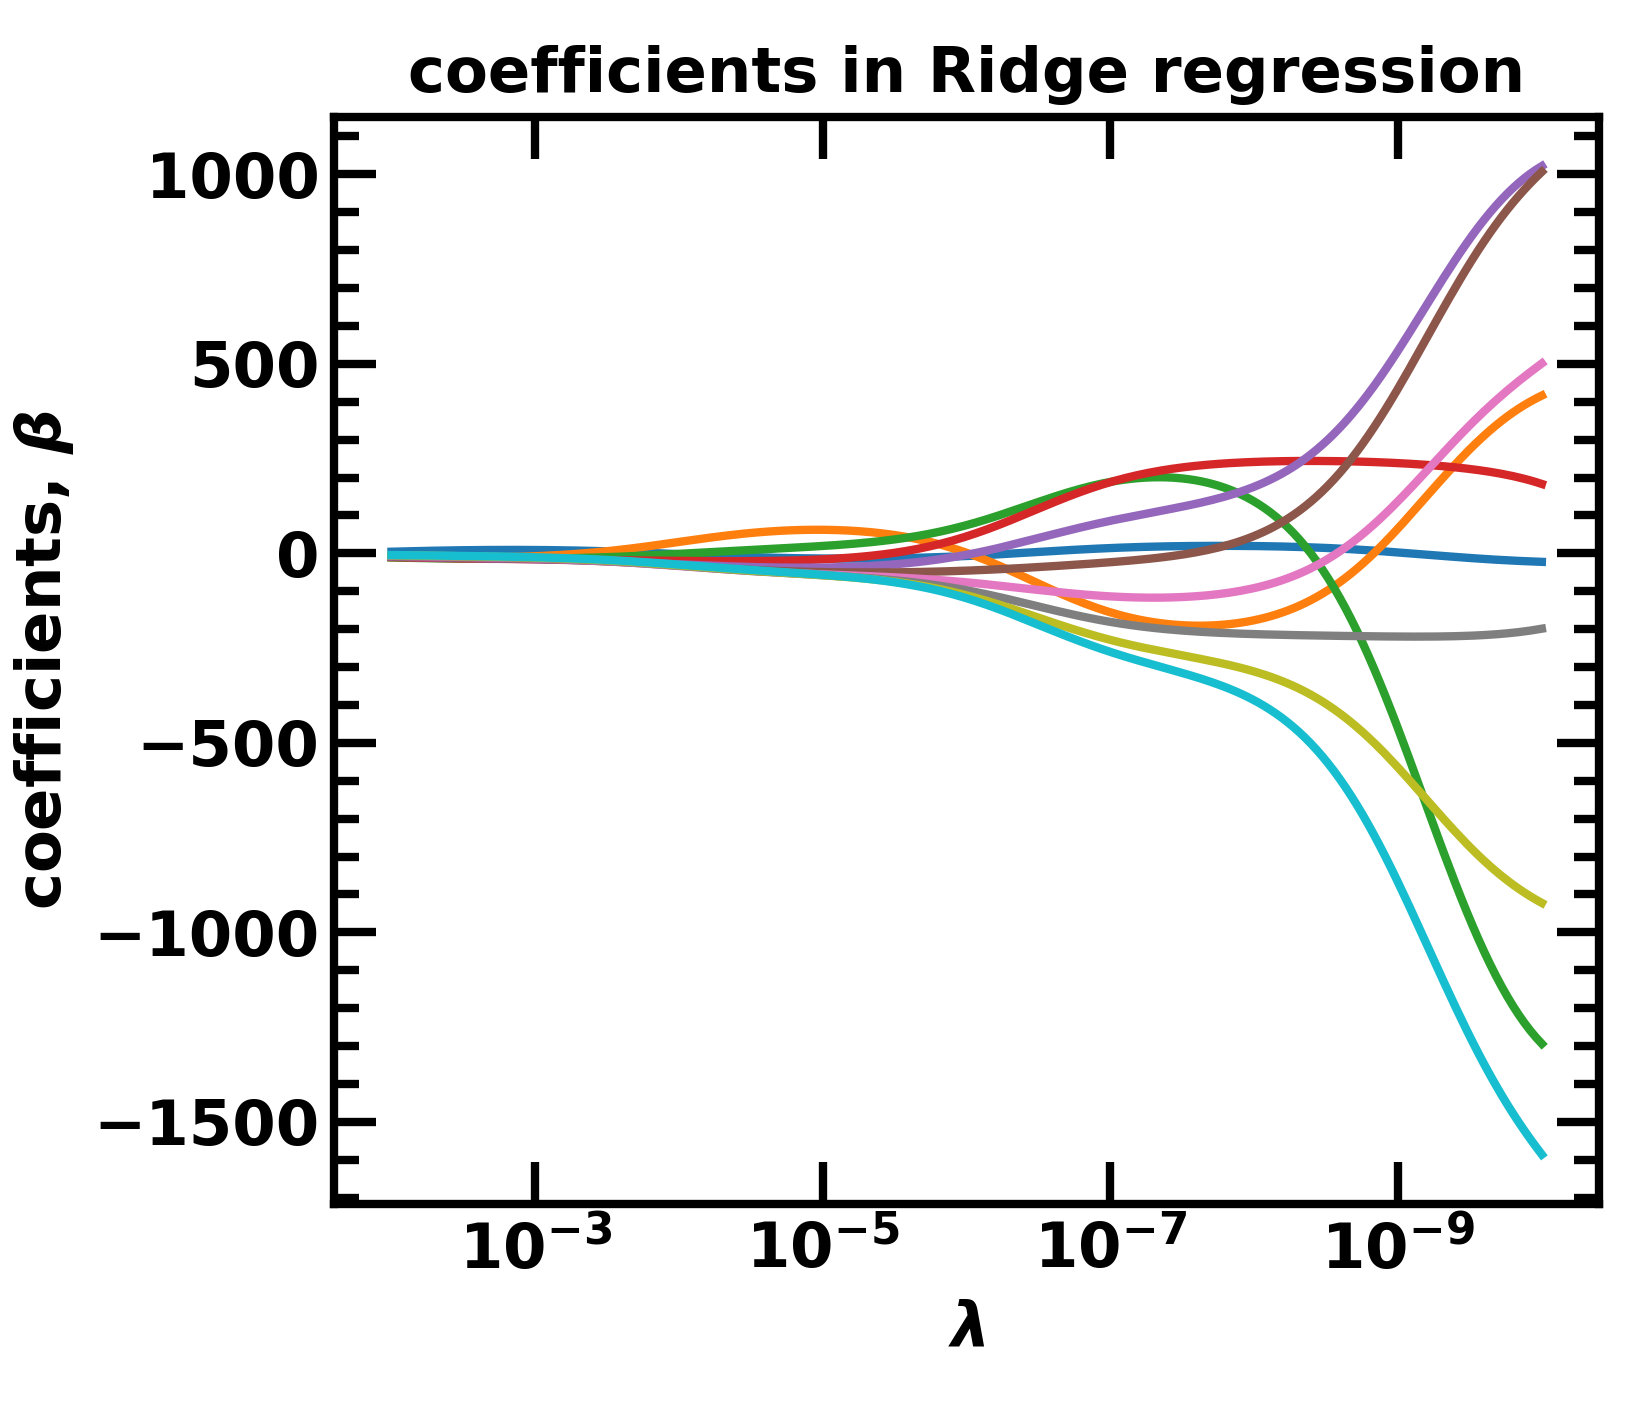
\includegraphics[width=0.6\linewidth]{../figures/statisticalLearning/linearModelRegression/ridgeCoefficientPath}
	\caption{Values of $\beta$ as we decreasing the regularizer parameter $\lambda$. code: ridgeRegressionPath.py}
	\label{fig:ridgeCoefficientPath}
\end{figure}


\subsubsection{The primal and dual form of ridge regression}

\begin{lemma}[the primal problem]
	\cite[494]{murphy2012machine}Let $x\in \R^D$ be some feature vector, and $X$ be the $N\times D$ design matrix. The goal is
	$$\min_{w} (y - Xw)^T(y - Xw) + \lambda \norm{w}^2,\lambda > 0$$
	with the optimal solution given as
	$$w = (X^TX + \lambda I)^{-1} X^Ty = (\sum_i x_ix_i^T + \lambda I)^{-1} X^Ty$$
\end{lemma}
\begin{proof}
	see \autoref{ch:theory-of-statistics:sec:linear-regression-analysis}.	
\end{proof}


\begin{lemma}[the dual problem]
	\cite[494]{murphy2012machine}\index{dual problem}
	Using matrix inversion lemma, $w = X^T(XX^T + \lambda I_N)^{-1}y$. Define $\alpha = (XX^T + \lambda I_N)^{-1}y$, then $w = X^T\alpha$. Moreover, given a new input $x$, 
	the prediction is $y = w^T x = \alpha^T X^T x = \sum_{i} \alpha_i x^T_i x$
\end{lemma}
\begin{proof}
	using the matrix inversion lemma can prove it.	
\end{proof}


\begin{remark}[advantages  of dual problems]\hfill
	\begin{itemize}
		\item The dual problem has advantage when $D\gg N$ in calculating $(XX^T + \lambda I_N)^{-1}$, which takes $O(N^3)$ whereas in primal form $(X^TX + \lambda I)^{-1}$ takes $O(D^3)$.
		\item The dual problem uses inner product in the formulation, which is useful when using kernel methods/tricks. 
	\end{itemize}
\end{remark}


%\subsection{Non-parametric method for regression}

\subsection{Lasso regression}

\begin{definition}[The Lasso regression]\index{Lasso regression}
	Consider \textbf{centered} data in the linear regression model. The ridge regression is to estimate $\hat{\beta}_{ridge}$ by minimizing
	$$\min_{\beta} \norm{Y - X\beta}_2^2 + \lambda \abs{\beta}.$$
\end{definition}


\begin{remark}[necessary of data preprocessing]\hfill
	\begin{itemize}
		\item Each column of $X$ data should be centered and divided by standard deviation.  
	\end{itemize}
\end{remark}

\begin{remark}[Effect of shrinkage]\hfill
	\begin{itemize}
		\item Let $X_j$ be the $j$ predicator. When $X_j$ is weakly related with $Y$, the Lasso pulls $\beta_j$ to zero faster than ridge regression.
	\end{itemize}
\end{remark}








\begin{lemma}[Lasso regression when inputs are orthogonal]
	
\end{lemma}










\subsection{Linear Gaussian systems}
Suppose we have two variables, $\vec{x}$ and $\vec{y}$.Let $\vec{x} \in \mathbb{R}^{D_x}$ be a hidden variable, and $\vec{y} \in \mathbb{R}^{D_y}$ be a noisy observation of $\vec{x}$. Let us assume we have the following prior and likelihood:
\begin{equation}\label{eqn:Linear-Gaussian-system}
\boxed{\begin{split}
	p(\vec{x})&=\mathcal{N}(\vec{x}|\vec{\mu}_x,\vec{\Sigma}_x) \\
	p(\vec{y}|\vec{x})&=\mathcal{N}(\vec{y}|\vec{W}\vec{x}+\vec{\mu}_y,\vec{\Sigma}_y)
	\end{split}}
\end{equation}
where $\vec{W}$ is a matrix of size $D_y \times D_x$. This is an example of a \textbf{linear Gaussian system}. We can represent this schematically as $\vec{x} \rightarrow \vec{y}$, meaning $\vec{x}$ generates $\vec{y}$. In this section, we show how to “invert the arrow”, that is, how to infer $\vec{x}$ from $\vec{y}$. We state the result below, then give several examples, and finally we derive the result. We will see many more applications of these results in later chapters.


\subsubsection{Statement of the result}
\begin{theorem}(\textbf{Bayes rule for linear Gaussian systems}). 
	Given a linear Gaussian system, as in Equation \ref{eqn:Linear-Gaussian-system}, the posterior $p(\vec{x}|\vec{y})$ is given by the following:
	\begin{equation}\label{eqn:Linear-Gaussian-system-posterior}
	\boxed{\begin{split}
		p(\vec{x}|\vec{y})&=\mathcal{N}(\vec{x}|\vec{\mu}_{x|y},\vec{\Sigma}_{x|y}) \\
		\vec{\Sigma}_{x|y}&=\vec{\Sigma}_x^{-1}+\vec{W}^T\vec{\Sigma}_y^{-1}\vec{W} \\
		\vec{\mu}_{x|y}&=\vec{\Sigma}_{x|y}\left[\vec{W}^T\vec{\Sigma}_y^{-1}(\vec{y}-\vec{\mu}_y)+\vec{\Sigma}_x^{-1}\vec{\mu}_x\right]
		\end{split}}
	\end{equation}
	In addition, the normalization constant $p(\vec{y})$ is given by
	\begin{equation}\label{eqn:Linear-Gaussian-system-normalizer}
	\boxed{
		p(\vec{y})=\mathcal{N}(\vec{y}|\vec{W}\vec{\mu}_x+\vec{\mu}_y,\vec{\Sigma}_y+\vec{W}\vec{\Sigma}_x\vec{W}^T)
	}
	\end{equation}
\end{theorem}

For the proof, see Section 4.4.3 TODO.


\section{Penalized linear regression: case studies}


\section{The exponential family}
\label{sec:exponential-family}

Before defining the exponential family, we mention several reasons why it is important:
\begin{itemize}
	\item{It can be shown that, under certain regularity conditions, the exponential family is the only family of distributions with finite-sized sufficient statistics, meaning that we can compress the data into a fixed-sized summary without loss of information. This is particularly useful for online learning, as we will see later.}
	\item{The exponential family is the only family of distributions for which conjugate priors exist, which simplifies the computation of the posterior (see Section \ref{sec:Bayes-for-the-exponential-family}).}
	\item{The exponential family can be shown to be the family of distributions that makes the least set of assumptions subject to some user-chosen constraints (see Section \ref{sec:Maximum-entropy-derivation-of-the-exponential-family}).}
	\item{The exponential family is at the core of generalized linear models, as discussed in Section \ref{sec:GLMs}.}
	\item{The exponential family is at the core of variational inference, as discussed in Section TODO.}
\end{itemize}


\subsection{Definition}
A pdf or pmf $p(\vec{x}|\vec{\theta})$,for $\vec{x} \in \mathbb{R}^m$ and $\vec{\theta} \in \mathbb{R}^D$, is said to be in the \textbf{exponential family} if it is of the form
\begin{align}
p(\vec{x}|\vec{\theta}) & =\dfrac{1}{Z(\vec{\theta})}h(\vec{x})\exp[\vec{\theta}^T\phi(\vec{x})] \\
& = h(\vec{x})\exp[\vec{\theta}^T\phi(\vec{x})-A(\vec{\theta})] \label{eqn:exponential-family}
\end{align}
where
\begin{align}
Z(\vec{\theta}) & =\int h(\vec{x})\exp[\vec{\theta}^T\phi(\vec{x})]\mathrm{d}\vec{x} \\
A(\vec{\theta}) & =\log Z(\vec{\theta})
\end{align}

Here $\vec{\theta}$ are called the \textbf{natural parameters} or \textbf{canonical parameters}, $\phi(\vec{x}) \in \mathbb{R}^D$ is called a vector of \textbf{sufficient statistics}, $Z(\vec{\theta})$ is called the \textbf{partition function}, $A(\vec{\theta})$ is called the \textbf{log partition function} or \textbf{cumulant function}, and $h(\vec{x})$ is the a scaling constant, often 1. If $\phi(\vec{x})=\vec{x}$, we say it is a \textbf{natural exponential family}.

Equation \ref{eqn:exponential-family} can be generalized by writing
\begin{equation}
p(\vec{x}|\vec{\theta}) = h(\vec{x})\exp[\eta(\vec{\theta})^T\phi(\vec{x})-A(\eta(\vec{\theta}))]
\end{equation}
where $\eta$ is a function that maps the parameters $\vec{\theta}$ to the canonical parameters $\vec{\eta}=\eta(\vec{\theta})$.If $\mathrm{dim}(\vec{\theta})<\mathrm{dim}(\eta(\vec{\theta}))$, it is called a \textbf{curved exponential family}, which means we have more sufficient statistics than parameters. If $\eta(\vec{\theta})=\vec{\theta}$, the model is said to be in \textbf{canonical form}. We will assume models are in canonical form unless we state otherwise.


\subsection{Examples}


\subsubsection{Bernoulli}
The Bernoulli for $x \in \{0,1\}$ can be written in exponential family form as follows:
\begin{equation}\begin{split}
\mathrm{Ber}(x|\mu)& =\mu^x(1-\mu)^{1-x} \\
& =\exp[x\log\mu+(1-x)\log(1-\mu)]
\end{split}\end{equation}
where $\phi(x)=(\mathbb{I}(x=0),\mathbb{I}(x=1))$ and $\vec{\theta}=(\log\mu,\log(1-\mu))$. 

However, this representation is \textbf{over-complete} since $\vec{1}^T\phi(x)=\mathbb{I}(x=0)+\mathbb{I}(x=1)=1$. Consequently $\vec{\theta}$ is not uniquely identifiable. It is common to require that the representation be \textbf{minimal}, which means there is a unique $\theta$ associated with the distribution. In this case, we can just define
\begin{align}
\mathrm{Ber}(x|\mu) & =(1-\mu)\exp\left(x\log\dfrac{\mu}{1-\mu}\right) \\
\text{where } \phi(x) & =x, \theta=\log\dfrac{\mu}{1-\mu}, Z=\dfrac{1}{1-\mu}  \nonumber
\end{align}

We can recover the mean parameter $\mu$ from the canonical parameter using
\begin{equation}
\mu=\mathrm{sigm}(\theta)=\dfrac{1}{1+e^{-\theta}}
\end{equation}


\subsubsection{Multinoulli}
We can represent the multinoulli as a minimal exponential family as follows:
\begin{equation*}\begin{split}
& \mathrm{Cat}(\vec{x}|\vec{\mu}) = \prod\limits_{k=1}^K = \exp\left(\sum\limits_{k=1}^K x_k\log\mu_k\right) \\
& = \exp\left[\sum\limits_{k=1}^{K-1} x_k\log\mu_k+  (1-\sum\limits_{k=1}^{K-1} x_k)\log(1-\sum\limits_{k=1}^{K-1} \mu_k)\right] \\
& = \exp\left[\sum\limits_{k=1}^{K-1} x_k\log\dfrac{\mu_k}{1-\sum_{k=1}^{K-1} \mu_k} + \log(1-\sum\limits_{k=1}^{K-1} \mu_k) \right] \\
& = \exp\left[\sum\limits_{k=1}^{K-1} x_k\log\dfrac{\mu_k}{\mu_K}+\log\mu_K\right] \text{, where } \mu_K \triangleq 1-\sum\limits_{k=1}^{K-1} \mu_k
\end{split}\end{equation*}

We can write this in exponential family form as follows:
\begin{align}
\mathrm{Cat}(\vec{x}|\vec{\mu}) & = \exp[\vec{\theta}^T\phi(\vec{x})-A(\vec{\theta})] \\
\vec{\theta} & \triangleq (\log\dfrac{\mu_1}{\mu_K},\cdots,\log\dfrac{\mu_{K-1}}{\mu_K}) \\
\phi(\vec{x}) & \triangleq (x_1,\cdots,x_{K-1})
\end{align}

We can recover the mean parameters from the canonical parameters using
\begin{align}
\mu_k & = \dfrac{e^{\theta_k}}{1+\sum_{j=1}^{K-1} e^{\theta_j}} \\
\mu_K & = 1- \dfrac{\sum_{j=1}^{K-1} e^{\theta_j}}{1+\sum_{j=1}^{K-1} e^{\theta_j}}=\dfrac{1}{1+\sum_{j=1}^{K-1} e^{\theta_j}}
\end{align}
and hence
\begin{equation}
A(\vec{\theta]} = -\log\mu_K=\log(1+\sum\limits_{j=1}^{K-1} e^{\theta_j})
\end{equation}


\subsubsection{Univariate Gaussian}
The univariate Gaussian can be written in exponential family form as follows:
\begin{align}
\mathcal{N}(x|\mu,\sigma^2) & =\dfrac{1}{\sqrt{2\pi}\sigma}\exp\left[-\dfrac{1}{2\sigma^2}(x-\mu)^2\right] \nonumber \\
& = \dfrac{1}{\sqrt{2\pi}\sigma}\exp\left[-\dfrac{1}{2\sigma^2}x^2+\dfrac{\mu}{\sigma^2}x-\dfrac{1}{2\sigma^2}\mu^2\right] \nonumber \\
& = \dfrac{1}{Z(\vec{\theta})}\exp[\vec{\theta}^T\phi(x)]
\end{align}
where
\begin{align}
\vec{\theta} & = (\dfrac{\mu}{\sigma^2}, -\dfrac{1}{2\sigma^2}) \\
\phi(x) & =(x,x^2) \\
Z(\vec{\theta}) & =\sqrt{2\pi}\sigma\exp(\dfrac{\mu^2}{2\sigma^2})
\end{align}


\subsubsection{Non-examples}
Not all distributions of interest belong to the exponential family. For example, the uniform distribution,$X \sim U(a,b)$, does not, since the support of the distribution depends on the parameters. Also, the Student T distribution (Section TODO) does not belong, since it does not have the required form.


\subsection{Log partition function}
An important property of the exponential family is that derivatives of the log partition function can be used to generate \textbf{cumulants} of the sufficient statistics.\footnote{The first and second cumulants of a distribution are its mean $\mathbb{E}[X]$ and variance $\mathrm{var}[X]$, whereas the first and second moments are its mean $\mathbb{E}[X]$ and $\mathbb{E}[X^2]$.} For this reason, $A(\vec{\theta})$ is sometimes called a \textbf{cumulant function}. We will prove this for a 1-parameter distribution; this can be generalized to a $K$-parameter distribution in a straightforward way. For the first derivative we have

For the second derivative we have
\begin{align}
\dfrac{\mathrm{d} A}{\mathrm{d} \theta} & = \dfrac{\mathrm{d}}{\mathrm{d} \theta}\left\{\log\int\exp\left[\theta\phi(x)\right]h(x)\mathrm{d}x\right\} \nonumber \\
& = \dfrac{\frac{\mathrm{d}}{\mathrm{d} \theta}\int\exp\left[\theta\phi(x)\right]h(x)\mathrm{d}x}{\int\exp\left[\theta\phi(x)\right]h(x)\mathrm{d}x} \nonumber \\
& = \dfrac{\int\phi(x)exp\left[\theta\phi(x)\right]h(x)\mathrm{d}x}{\exp(A(\theta))} \nonumber \\
& = \int \phi(x)\exp\left[\theta\phi(x)-A(\theta)\right]h(x)\mathrm{d}x \nonumber \\
& = \int \phi(x)p(x)\mathrm{d}x=\mathbb{E}[\phi(x)]
\end{align}

For the second derivative we have
\begin{align}
\dfrac{\mathrm{d}^2 A}{\mathrm{d} \theta^2} & = \int \phi(x)\exp\left[\theta\phi(x)-A(\theta)\right]h(x)\left[\phi(x)-A'(\theta)\right]\mathrm{d}x \nonumber \\
& = \int \phi(x)p(x)\left[\phi(x)-A'(\theta)\right]\mathrm{d}x \nonumber \\
& = \int \phi^2(x)p(x)\mathrm{d}x-A'(\theta)\int \phi(x)p(x)\mathrm{d}x \nonumber \\
& = \mathbb{E}[\phi^2(x)]-\mathbb{E}[\phi(x)]^2=\mathrm{var}[\phi(x)]
\end{align}

In the multivariate case, we have that
\begin{equation}
\dfrac{\partial^2 A}{\partial \theta_i \partial \theta_j}=\mathbb{E}[\phi_i(x)\phi_j(x)]-\mathbb{E}[\phi_i(x)]\mathbb{E}[\phi_j(x)]
\end{equation}
and hence
\begin{equation}
\nabla^2A(\vec{\theta}) = \mathrm{cov}[\phi(\vec{x})]
\end{equation}

Since the covariance is positive definite, we see that $A(\vec{\theta})$ is a convex function (see Section \ref{sec:Convexity}).


\subsection{MLE for the exponential family}
The likelihood of an exponential family model has the form
\begin{equation}
p(\mathcal{D}|\vec{\theta})=\left[\prod\limits_{i=1}^N h(\vec{x}_i)\right]g(\vec{\theta})^N\exp\left[\vec{\theta}^T\left(\sum\limits_{i=1}^N \phi(\vec{x}_i)\right)\right]
\end{equation}

We see that the sufficient statistics are $N$ and
\begin{equation}
\phi(\mathcal{D})=\sum\limits_{i=1}^N \phi(\vec{x}_i)=(\sum\limits_{i=1}^N \phi_1(\vec{x}_i),\cdots,\sum\limits_{i=1}^N \phi_K(\vec{x}_i))
\end{equation}

The \textbf{Pitman-Koopman-Darmois theorem} states that, under certain regularity conditions, the exponential family is the only family of distributions with finite sufficient statistics. (Here, finite means of a size independent of the size of the data set.)

One of the conditions required in this theorem is that the support of the distribution not be dependent on the parameter.


\section{Kernel regression}
\subsection{Smoothing kernels}
\begin{definition}[smoothing kernel]\index{smoothing kernel}\cite[509]{murphy2012machine}
	A smoothing kernel is a function of one argument which satisfies the following properties:
	\begin{itemize}
		\item $\int k(x) dx= 1$
		\item (symmetric property)$\int xk(x) dx = 0$
		\item $\int x^2k(x) dx > 0$
	\end{itemize}
\end{definition}

\begin{lemma}[basic shift and scaling property of smoothing kernel]
	Given a smoothing kernel $k$, we have:
	\begin{itemize}
		\item $\int k(y-y_0)dy = 1$
		\item $\int yk(y - y_0)dy = y_0$
		\item $$k_h = \frac{1}{h^D}k(\frac{x}{h})$$ is a also a smoothing kernel with bandwidth parameter $h$, where $D$ is the dimensionality. 
	\end{itemize}
\end{lemma}


\begin{example}\hfill
	\begin{itemize}
		\item (Gaussian kernel)
		$$k_h(x) = \frac{1}{h^D(2\pi)^{D/2}} \prod_{j=1}^D \exp(-\frac{1}{2h^2}x_j^2),x\in \R^D$$
		\item (boxcar kernel)
		$$k(x) = I(\abs{x} \leq 1)$$
		\item (tri-cube kernel)
		$$k(x) = \frac{70}{81}(1 - \abs{x}^3)^3I(\abs{x}\leq 1)$$
	\end{itemize}
\end{example}




\subsection{Kernel regression}
$$f(x) = E[y|x] = \int y p(y|x) dy = \frac{\int y p(x,y)dy}{\int p(x,y)dy}$$

Using kernel density estimation to approximate $p(x,y)$, we have

$$p(x,y) \approx \frac{1}{N} \sum_{i=1}^N k_h(x-x_i)k_h(y-y_i)$$

Then
\begin{align*}
f(x) &= \frac{\frac{1}{N} \sum_{i=1}^N k_h(x-x_i)\int yk_h(y-y_i)dy}{\frac{1}{N} \sum_{i=1}^N k_h(x-x_i)\int k_h(y-y_i)dy}\\
&= \frac{\frac{1}{N} \sum_{i=1}^N k_h(x-x_i)y_i}{\frac{1}{N} \sum_{i=1}^N k_h(x-x_i)}\\
&=\sum_{i=1}^N w_i(x)y_i
\end{align*}
where
$$w_i = \frac{k_h(x-x_i)}{ \sum_{i=1}^N k_h(x-x_i)}.$$



The polynomial model is given as
$$P_x(u,a) = a_0 + a_1(u-x) + \frac{a_2}{2!}(u-x)^2 + ... + \frac{a_p}{p!}(u-x)^p$$
and the prediction at $u=x$ is $a_0$.


$$X_x = \begin{pmatrix}
1 & x_1-x & \dots & \frac{(x_1-x)^p}{p!}\\ 
1 & x_2-x & \dots & \frac{(x_2-x)^p}{p!}\\ 
\vdots & \vdots & \ddots & \vdots \\ 
1 & x_n-x & \dots & \frac{(x_n-x)^p}{p!}
\end{pmatrix}$$
By minimizing the weighted cost
$$(Y-X_x a(x))^TW_x(Y - X_x a(x))$$
where $$W_x = diag(w_1(x),...,w_N(x),w_i = \frac{k_h(x-x_i)}{ \sum_{i=1}^N k_h(x-x_i)}.$$
we get
$$\hat{a}(x) = (X_x^TW_xX_x)^{-1}X_x^TW_xY$$
and
$$\hat{a}_0 = e_1^T(X_x^TW_xX_x)^{-1}X_x^TW_xY$$


\begin{remark}[interpretation]
	In kernel regression, we have a family of polynomials parameterized by $x$. For every $x$, we need to solve the weighted least square to get a new polynomial.
\end{remark}

\begin{remark}[how prediction works?]\hfill
	Consider we use kernel regression to predict response at a new $x$: if $x = x_i,i\in \{1,...,N\}$, then $\hat{y} = y_i$; otherwise, $\hat{y} = \hat{a}_0 = e_1^T(X_x^TW_xX_x)^{-1}X_x^TW_xY. $
\end{remark}



\section{Note on bibliography}


\printbibliography
\end{refsection}




\begin{refsection}
\startcontents[chapters]	
	\chapter{Linear models for classification}\label{ch:StatisticalLearning-linear-models}
\printcontents[chapters]{}{1}{}


\section{Gaussian discriminate analysis}





\subsection{Linear Gaussian discriminant model}
\subsubsection{The model}
\begin{definition}[linear discriminant model]\index{linear discriminant model}\cite[139]{james2013introduction}
	Let the training data consists of $N$ pairs $(x_1,y_1),(x_2,y_2),...,(x_N,y_N)$, with $x_i \in \R^p, y_i \in \{1,...,K\}$. Then the \textbf{linear Gaussian discriminant model} models the pdf as
	\begin{align*}
	f(X|Y=1)&\sim MN(\mu_1,\Sigma),\\
	f(X|Y=2)& \sim MN(\mu_2,\Sigma),\\
	\cdots & \\
	f(X|Y=K)& \sim MN(\mu_K,\Sigma).
	\end{align*}
	where $\mu_1,...,\mu_K\in \R^p, \Sigma\in \R^{p\times p}$ and prior probabilities of classes $\pi_1,...,\pi_K$ are model parameters.
	Based on Bayes rule, we have the posterior probability
	$$Pr(Y = k|X=x) = \frac{f(X=x|Y=k)\pi_k}{\sum_{k=1}^K f(X=x|Y=k)\pi_k}.$$
\end{definition}




\begin{lemma}[Bayesian inference for classification]\cite[106]{murphy2012machine}
	Consider a Gaussian linear discriminant model with $K$ classes. Let $f_k$ denote $f(X|y=k)$. Then
	\begin{itemize}
		\item the distribution of class label $Y$ given $x$ is given by
		$$P(Y=k|X=x) = \frac{\pi_k f_k(x)}{\sum_{i=1}^{k}\pi_k f_k(x)},$$
		which can be use to predict $y$ label given $x$. Here $\pi_1,...,\pi_K$ are the prior probabilities on $Y$. 
	\end{itemize}	
\end{lemma}



\begin{remark}[Probability comparison and the linearity?]
	Denote $f_k(x) = f(X|Y=k)$.	
	Consider we want to compare $P(Y=1|x) > P(Y=2|x)$ via
	\begin{align*}
	\ln \frac{P(Y=1|x)}{P(Y=2|x)} &= \ln \frac{f_1(x)\pi_1}{f_2(x)\pi_2}\\
	&= \ln \frac{\pi_1}{\pi_2} + \frac{1}{2}((x-\mu_2)^T\Sigma^{-1}(x-\mu_2) - (x-\mu_1)^T\Sigma^{-1}(x-\mu_1)) \\
	&= \ln \frac{\pi_1}{\pi_2} + x\Sigma^{-1}(\mu_2-\mu_1) + \frac{1}{2}\mu_2^T\Sigma^{-1}\mu_2 - \frac{1}{2}\mu_1^T\Sigma^{-1}\mu_1)
	\end{align*}
	where quadratic terms of $x$ are canceled out.
\end{remark}


\begin{method}[linear discriminate functions for classification]
	Suppose model parameters $\mu, \Sigma, \pi$ are given. Given a new input $x$, we can use following way to classify $x$.
	\begin{itemize}
		\item Define \textbf{linear discriminate functions} for each class $K$ as
		$$\delta_k(x) = x^T\Sigma^{-1}\mu_k - \frac{1}{2}\mu_k^T\Sigma^{-1}\mu_k + \log \pi_k.$$
		\item $x$ belongs to class $C$ that has the largest $\delta_k(x)$. 
	\end{itemize}
\end{method}


\subsubsection{Model parameter estimation}


\begin{lemma}[maximum likelihood estimator]
	\begin{itemize}
		\item $$\hat{\pi}_k = \frac{N_k}{N}, N_k = \sum_{i=1}^N \bm{1}(y_i = k).$$
		\item $$\hat{\mu}_k = \frac{\sum_{i:y_i =k} x_i}{N_k}.$$
		\item $$\hat{\Sigma} = \sum_{k=1}^K\sum_{i:y_i=k}\frac{(x_i - \hat{\mu}_k)(x_i - \hat{\mu}_k)^T}{N-K}.$$
	\end{itemize}	
\end{lemma}




\begin{corollary}[Estimation of parameters]\cite[108]{murphy2012machine}
	For the case $p = 1$, we can estimate $\hat{\mu}, \hat{\sigma}^2$ using following procedures:
	\begin{itemize}
		\item $$\hat{\mu}_k = \frac{1}{n_k}\sum_{i:y_i =k} x_i.$$ 
		\item $$\hat{\sigma}^2 = \frac{1}{n-K}\sum_{k=1}^K \sum_{i:y_i =k} (x_i - \hat{\mu}_k)^2.$$ 
	\end{itemize}
\end{corollary}


\subsubsection{Geometry of decision boundary}

\begin{remark}[geometry of decision boundary]\hfill
	\begin{itemize}
		\item For two-class classification problem, the decision boundary determined by $\delta_1(x) = \delta_2(x)$ is a hyperplane given by 
		$$	x^T\Sigma^{-1}(\mu_2-\mu_1) + \ln \frac{\pi_1}{\pi_2} +  \frac{1}{2}\mu_2^T\Sigma^{-1}\mu_2 - \frac{1}{2}\mu_1^T\Sigma^{-1}\mu_1) = 0.$$
		This hyperplane has normal vector $\Sigma^{-1}(\mu_2-\mu_1)$ and passing $\frac{\mu_1 + \mu_2}{2}$ when $\pi_1 = \pi_2$ since $$\delta_1(\frac{\mu_1 + \mu_2}{2}) = \delta_2(\frac{\mu_1 + \mu_2}{2}).$$
		\item Similarly, for multiple-class classification problem, the decision boundary between any pair of Gaussian distributions are hyperplane; all hyperplanes will intersect at the same point (or line, plane, depending on dimensionality of input space.) 
		\item For a three-class classification problem with 2D input space. Three decision boundaries will intersect at the same point; it can be showed:
		Suppose $x_0$ satisfies 
		$$\delta_1(x_0) = \delta_2(x_0), \delta_1(x_0) = \delta_3(x_0),$$
		then $x_0$ also satisfies
		$$\delta_2(x_0) = \delta_3(x_0).$$
		
	\end{itemize}	
\end{remark}

\begin{figure}[H]
	\centering
	\begin{subfigure}[t]{0.45\textwidth}
		\centering
		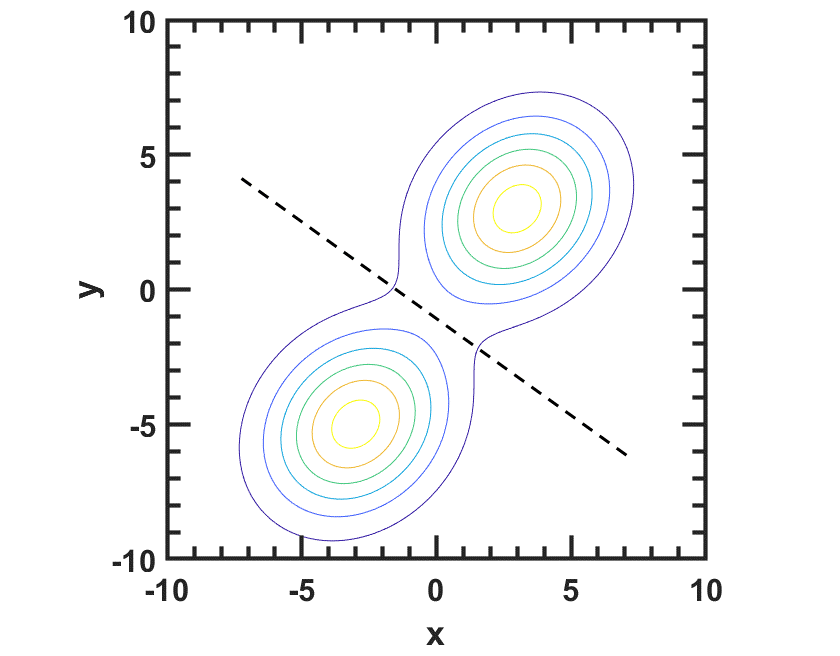
\includegraphics[width=1\linewidth]{../figures/statisticalLearning/linearModelClassification/linearGaussianDiscriminateDecisionBoundaryDemo2DOneOverlay}
		\caption{Decision boundary of a two-class classification problem. The conditional distributions are represented by the contours of the Gaussian distribution.}
	\end{subfigure}\quad
	\begin{subfigure}[t]{0.45\textwidth}
		\centering
		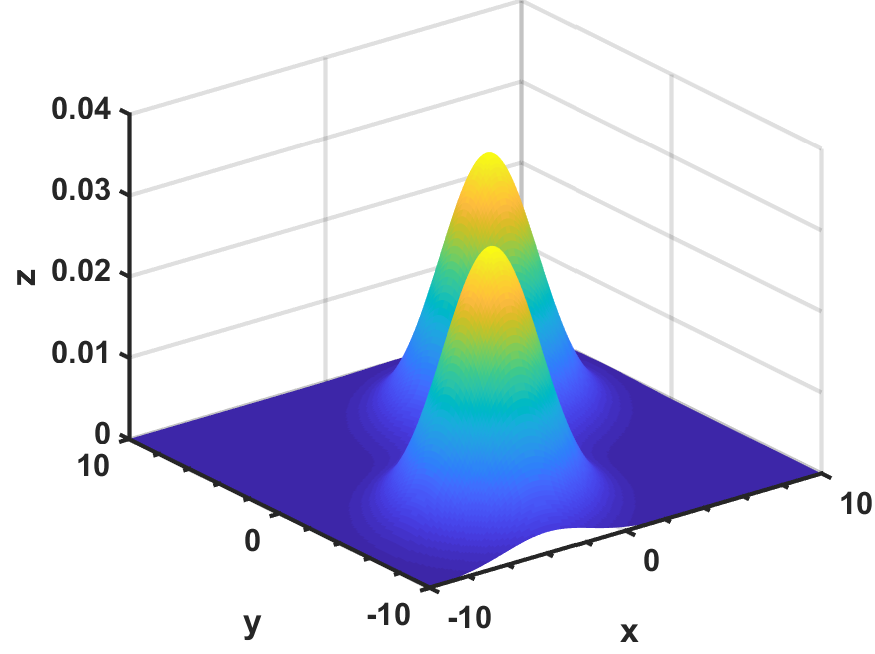
\includegraphics[width=1\linewidth]{../figures/statisticalLearning/linearModelClassification/linearGaussianDiscriminateDecisionBoundaryDemo3DOne}
		\caption{ A 3D view of the conditional distributions.}
	\end{subfigure}\quad
	\begin{subfigure}[t]{0.45\textwidth}
		\centering
		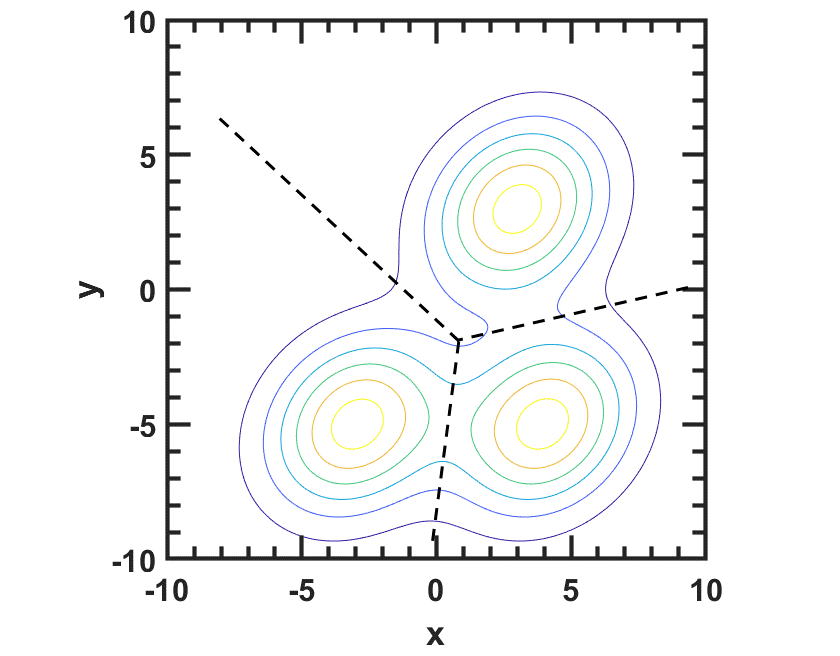
\includegraphics[width=1\linewidth]{../figures/statisticalLearning/linearModelClassification/linearGaussianDiscriminateDecisionBoundaryDemo2DTwoOverlay}
		\caption{Decision boundary of a three-class classification problem. The conditional distributions are represented by the contours of the Gaussian distribution.}
	\end{subfigure}\quad
	\begin{subfigure}[t]{0.45\textwidth}
		\centering
		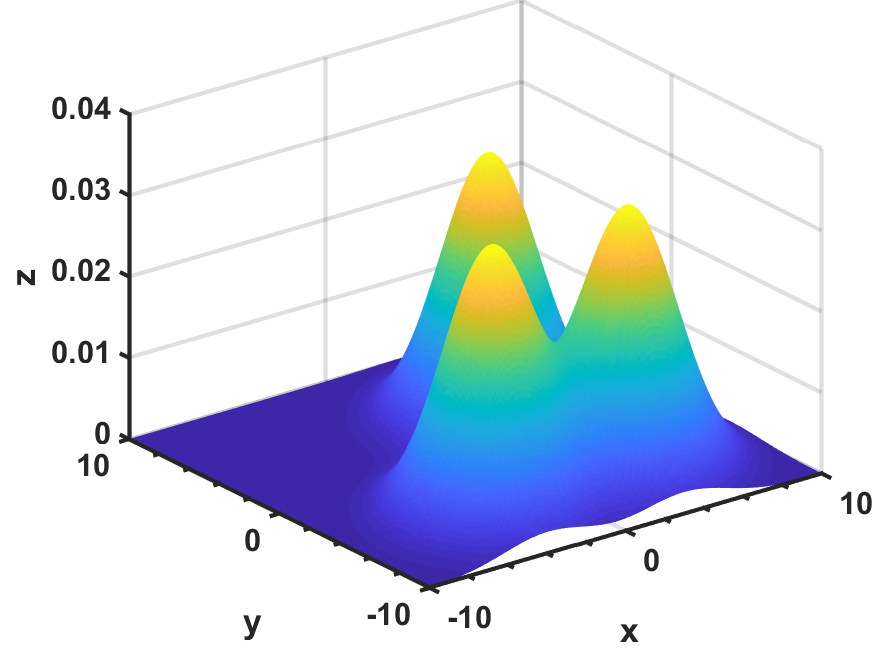
\includegraphics[width=1\linewidth]{../figures/statisticalLearning/linearModelClassification/linearGaussianDiscriminateDecisionBoundaryDemo3DTwo}
		\caption{A 3D view of the conditional distributions.}
	\end{subfigure}
	\caption{Geometry of decision boundary.}
	\label{fig:linearGaussianDiscriminateModeDecisionBoundaryDemo}
\end{figure}


\subsection{Quadratic Gaussian discriminant model}
\subsubsection{The model}
\begin{definition}[quadratic discriminant model]\index{quadratic discriminant model}\cite[146]{james2013introduction}
	Let the training data consists of $N$ pairs $(x_1,y_1),(x_2,y_2),...,(x_N,y_N)$, with $x_i \in \R^p, y_i \in \{1,...,K\}$. Then the Gaussian Quadratic discriminant model models the pdf as
	\begin{align*}
	f(X|Y=1)&\sim MN(\mu_1,\Sigma_1),\\
	f(X|Y=2)&\sim MN(\mu_2,\Sigma_2),\\
	\cdots&\\
	f(X|Y=K)& \sim MN(\mu_2,\Sigma_K)
	\end{align*}
	where $\mu_1,...,\mu_K\in \R^p, \Sigma_1,\Sigma_2,...,\Sigma_K \in \R^{p\times p}$ and prior probabilities of classes $\pi_1,...,\pi_K$ are model parameters are model parameters.
	Based on Bayes rule, we have
	$$P(Y=k|X=x) = \frac{\pi_k f_k(x)}{\sum_{i=1}^{k}\pi_k f_k(x)},$$
	which can be use to predict $y$ label given $x$. Here $\pi_1,...,\pi_K$ are the prior probabilities on $Y$. 
\end{definition}


\begin{remark}[difference between linear model and quadratic model]
	In quadratic model, we assume each class also has its own covariance matrix as model parameters; whereas in linear model, we assume all classes share the same covariance matrix. 
\end{remark}


\begin{remark}[probability comparison and quadratic discriminate function]
	Denote $f_k(x) = f(X|Y=k)$.	
	Consider we want to compare $P(Y=1|x) > P(Y=2|x)$ via
	$$\ln \frac{P(Y=1|x)}{P(Y=2|x)} = \delta_1(x) - \delta_2(x),
	$$
	where $$\delta_k(x) = -\frac{1}{2}\ln \abs{\Sigma_k} - \frac{1}{2}(x-\mu_k)^T\Sigma_k^{-1}(x-\mu_k) + \ln \pi_k,$$ is called quadratic discriminate function.
\end{remark}


\begin{method}[classification via discriminate function]
	Suppose model parameters $\mu, \Sigma, \pi$ are given. Given a new input $x$, we can use following way to classify $x$.
	\begin{itemize}
		\item Define \textbf{linear discriminate functions} for each class $K$ as
		$$\delta_k(x) = -\frac{1}{2}\ln \abs{\Sigma_k} - \frac{1}{2}(x-\mu_k)^T\Sigma_k^{-1}(x-\mu_k) + \ln \pi_k.$$
		\item $x$ belongs to class $C$ that has the largest $\delta_k(x)$. 
	\end{itemize}
\end{method}



\subsubsection{Model parameter estimation}


\begin{lemma}[maximum likelihood estimator]
	\begin{itemize}
		\item $$\hat{\pi}_k = \frac{N_k}{N}, N_k = \sum_{i=1}^N \bm{1}(y_i = k).$$
		\item $$\hat{\mu}_k = \frac{\sum_{i:y_i =k} x_i}{N_k}.$$
		\item $$\hat{\Sigma} = \sum_{k=1}^K\sum_{i:y_i=k}\frac{(x_i - \hat{\mu}_k)(x_i - \hat{\mu}_k)^T}{N-K}.$$
	\end{itemize}	
\end{lemma}




\begin{corollary}[Estimation of parameters]\cite[108]{murphy2012machine}
	For the case $p = 1$, we can estimate $\hat{\mu}, \hat{\sigma}^2$ using following procedures:
	\begin{itemize}
		\item $$\hat{\mu}_k = \frac{1}{n_k}\sum_{i:y_i =k} x_i.$$ 
		\item $$\hat{\sigma}^2 = \frac{1}{n-K}\sum_{k=1}^K \sum_{i:y_i =k} (x_i - \hat{\mu}_k)^2.$$ 
	\end{itemize}
\end{corollary}




\subsection{Regularized LDA}





\section{Linear discriminate analysis (LDA) }


Fisher linear discriminants are derived with the goal to find a low dimensional representation of the origin data that maximizes the class separability. As a result, classification rules can be constructed more naturally on the basis of the low dimension representation instead of the original data.


\subsection{One dimensional linear discriminant}
\subsubsection{Basics}
\begin{definition}[Fisher linear discriminant problem]\index{Fisher linear discriminant}
	Consider a set of input data $x_1,...,x_N\in \R^D$ being classified as two classes such that $y_i\in \{1,2\}$ and the following definition	
	\begin{itemize}
		\item Between-class scatter matrix
		$$S_B = (\mu_2 - \mu)(\mu_2-\mu)^T, \mu_i = \frac{1}{N_i}\sum_{j:y_j=i} x_j.$$
		\item Within-class scatter matrix
		$$S_W = \underbrace{\sum_{i:y_i=1} (x_i - \mu_1)(x_i - \mu_1)^T}_{S_1,  class~1~scatter~matrix} + \underbrace{\sum_{i:y_i=2} (x_i - \mu_2)(x_i - \mu_2)^T}_{S_2, ~class~2~scatter~matrix}.$$
	\end{itemize}
	
	
	The goal is to seek $w\in \R^D$ such that the projection of $x$ onto $w$ maximize the separability of the projections $w^Tx_1, w^Tx_2,..., w^Tx_N$. The vector $w$ is known as \textbf{linear discriminant}. 
	
	Or equivalently, the goal is to maximize projected mean distance over total within-class \textbf{projected scattering} via maximizing the following \textbf{Fisher criterion function}:
	$$J(w) = \frac{\abs{w^T(\mu_2-\mu_1)}^2}{w^T(S_1+S_2)w} =\frac{w^TS_Bw}{w^TS_ww}.$$
\end{definition}


\begin{figure}[H]
	\centering
	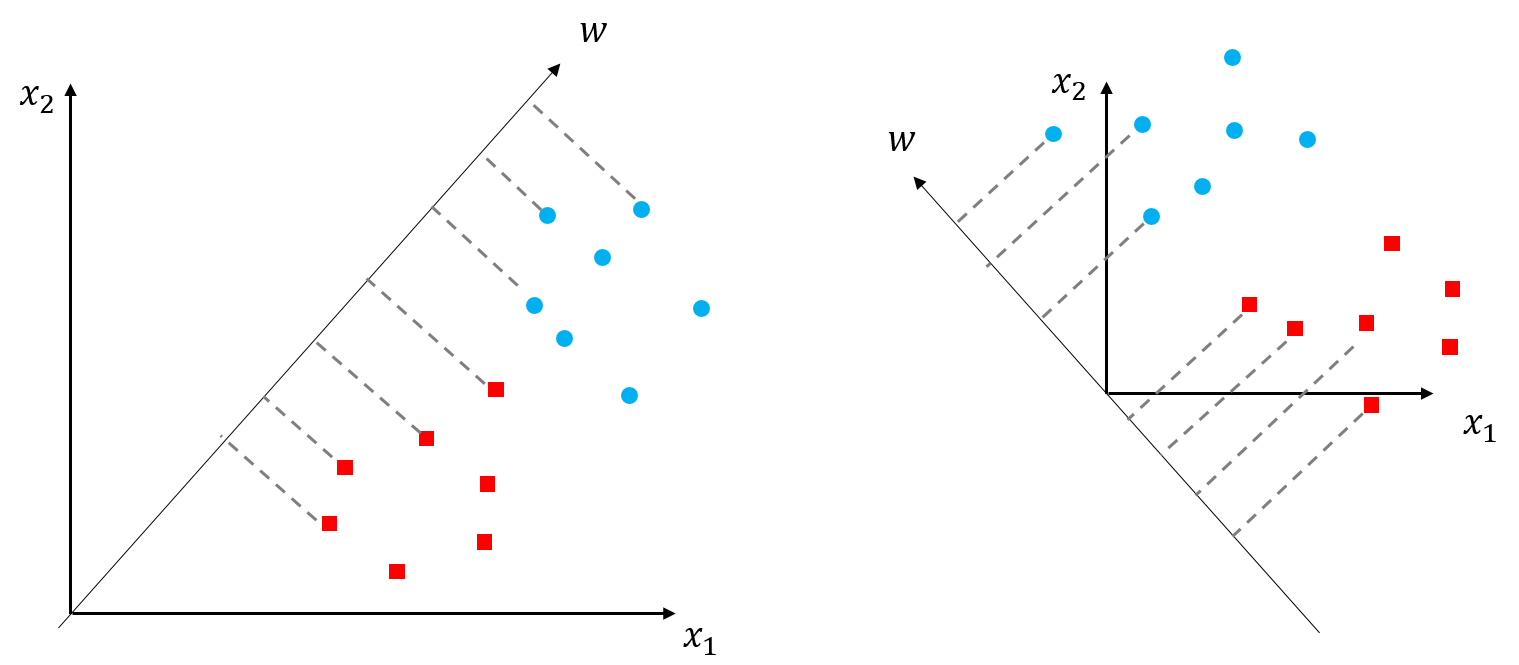
\includegraphics[width=0.8\linewidth]{../figures/statisticalLearning/linearModelClassification/linearDiscriminateVectorDemo}
	\caption{The linear discriminants that maximizing the separability for 2D sample points belonging to two classes. }
	\label{fig:lineardiscriminatevectordemo}
\end{figure}


\begin{lemma}[optimality condition for Fisher criterion function]\cite[186]{bishop2006pattern}\label{ch:statistical-learning:th:OptimalityConditionFisherCriterion}
	The optimal $w^*$, known as linear Fisher discriminant, that maximizes
	$$J(w) = \frac{w^TS_Bw}{w^TS_Ww}$$
	has following properties (assuming $S_W$ is invertible)
	\begin{itemize}
		\item The first-order optimality condition gives $S_w^{-1}S_Bw^* = Jw^*$
		\item The direction of $w^*$ is given by\footnote{note that here we mean $w^* = c S_W^{-1}(\mu_2 - \mu_1)$; $c$ is chosen such that $S_w^{-1}S_Bw^* = Jw^*$. However, the value $J$ is scale invariant.}
		$$w^* \propto S_W^{-1}(\mu_2 - \mu_1).$$
		\item Let $v$ be the eigenvector of $S_w^{-1}S_B$ and $\lambda$ be the associated eigenvalue\footnote{$S_w^{-1}S_B$ is of rank 1; therefore it only has one eigen-pair.}, then 
		$$w^* = v, J^*=\lambda.$$
	\end{itemize}	
\end{lemma}
\begin{proof}
	(1)	
	Take the derivative of $J(w)$ with respect to $w$, we have
	$$\frac{\Pa J}{\Pa w} = -\frac{2S_Ww(w^TS_Bw)}{(w^TS_Ww)^2} + \frac{2S_Bw}{(w^TS_Ww)} = 0,$$
	which gives
	\begin{align*}
	&2S_ww(w^TS_Bw) - 2S_Bw(w^TS_Ww) = 0 \\
	\implies& S_Bw = JS_Ww \\
	\implies& S_w^{-1}S_Bw = Jw
	\end{align*}
	(2)	
	Note that
	\begin{align*}
	Jw &= S_W^{-1}S_Bw\\
	&= S_W^{-1}(m_2 - m)\underbrace{(\mu_2-\mu)^Tw}_{c\in\R}\\
	\implies w &=  S_W^{-1}(\mu_2 - \mu)c/J   \propto S_W^{-1} (\mu_2-\mu_1).
	\end{align*}
	(3)
	Based on the eigenvector/eigenvalue definition, we have
	$$S_W^{-1}S_B w^* = \lambda w^* \implies S_B w^* = \lambda S_W w^*.$$
	Then, 
	$$J^* = \frac{[w^*]^TS_Bw^*}{[w^*]^TS_Ww^*} = \frac{[w^*]^T\lambda S_W w^*}{[w^*]^TS_Ww^*} = \lambda. $$
	
	All items can also be proved using generalized Rayleigh quotients (\autoref{ch:linearalgebra:th:GeneralizedRaylleighquotient}).
\end{proof}

\begin{remark}[interpretation]\hfill
	\begin{itemize}
		\item The linear Fisher discriminant is a direction that has the maximum between-class variance over within-class variance. The idea is similar in calculating top principal eigenvectors in PCA(\autoref{ch:statistical-learning:sec:PCA}).
		\item Given an optimal $w$, the discriminant function is $$y = w^Tx + w_0,$$
		where $w_0\in\R$ is such a value that minimizes the classification error.
	\end{itemize}
\end{remark}




\subsubsection{Application in classification}

\begin{lemma}[distance metric in the projected coordinates]
	Let $w$ be the Fisher linear discriminant and $x\in\R^D$ be a new input.	It follows that
	\begin{itemize}
		\item 	$w = S_W^{-1/2}e$, $e$ is the unit eigenvector of $S_W^{-1/2}S_BS_W^{-1/2}$.
		\item  The distance to mean in the projected coordinates is
		$$d_1(x) = \abs{w^T(x - \mu_1)}^2 = (x-\mu_1)^TS_W^{-1}(x-\mu_1)^T,$$
		$$d_2(x) = \abs{w^T(x - \mu_2)}^2 = (x-\mu_2)^TS_W^{-1}(x-\mu_2)^T.$$
	\end{itemize}	
\end{lemma}
\begin{proof}
	(1)	From \autoref{ch:statistical-learning:th:OptimalityConditionFisherCriterion}, we know that $w$ is the eigenvector of $S_W^{-1}S_B$ such that
	\begin{align*}
	S_W^{-1}S_B w &= \lambda w \\
	S_W^{-1}S_B S_W^{-1/2}e &= \lambda S_W^{-1/2}e \\
	S_W^{-1/2}S_B S_W^{-1/2}e &= \lambda e 
	\end{align*}
	(2) 
	\begin{align*}
	d_1 &= \abs{w^T(x - \mu_1)}^2 \\
	&= (x-\mu_1)^TS_W^{-1/2}e^TeS_W^{-1/2}(x-\mu_1)^T \\
	&= (x-\mu_1)^TS_W^{-1}(x-\mu_1)^T 
	\end{align*}
\end{proof}



\begin{method}[Binary classification using Fisher linear discriminant]
	Consider a set of input data $x_1,...,x_N\in \R^D$ being classified as two classes $\cC_1$ and $\cC_2$. Let $w$ be the Fisher linear discriminant. The classification rule is to assign $x$ to the class $i$ if the projected distance $w^T(x-\mu_i)$ is the smallest.
	
	More formally, 
	\begin{itemize}
		\item  Define the distance to mean in the projected coordinates as
		$$d_1(x) = \abs{w^T(x - \mu_1)}^2 = (x-\mu_1)^TS_W^{-1}(x-\mu_1)^T,$$
		$$d_2(x) = \abs{w^T(x - \mu_2)}^2 = (x-\mu_2)^TS_W^{-1}(x-\mu_2)^T.$$
		\item The classification rule is: if $d_1(x)\leq d_2(x)$, then $x$ belongs to class 1; otherwise class 2.
	\end{itemize}	
\end{method}


\begin{remark}[connection to Gaussian discriminant method] Consider the situation that the individual within-class scattering matrix $S_1 = S_2 = \Sigma$.
	In the Gaussian discriminant model, the \textbf{linear discriminate functions} for each class $k$ as
	$$\delta_k(x) = x^T\Sigma^{-1}\mu_k - \frac{1}{2}\mu_k^T\Sigma^{-1}\mu_k + \log \pi_k,$$
	or equivalently, 
	\begin{align*}
	\delta_k(x) - \frac{1}{2}x^T\Sigma^{-1}x  &= -\frac{1}{2}(x-\mu_k)^T\Sigma^{-1}(x-\mu_k) + \log \pi_k \\
	&= -\frac{1}{2}(x-\mu_k)^T(\frac{1}{2}S_W)^{-1}(x-\mu_k) + \log \pi_k \\
	&= -d_k(x) + \log \pi_k \\
	\end{align*}
	
	Therefore, when all the priors are equal; that is, $\pi_k = 1/2$, the linear discriminate function and the distance function give the same classification result.
\end{remark}




\subsubsection{Possible issues}



\begin{figure}[H]
	\centering
	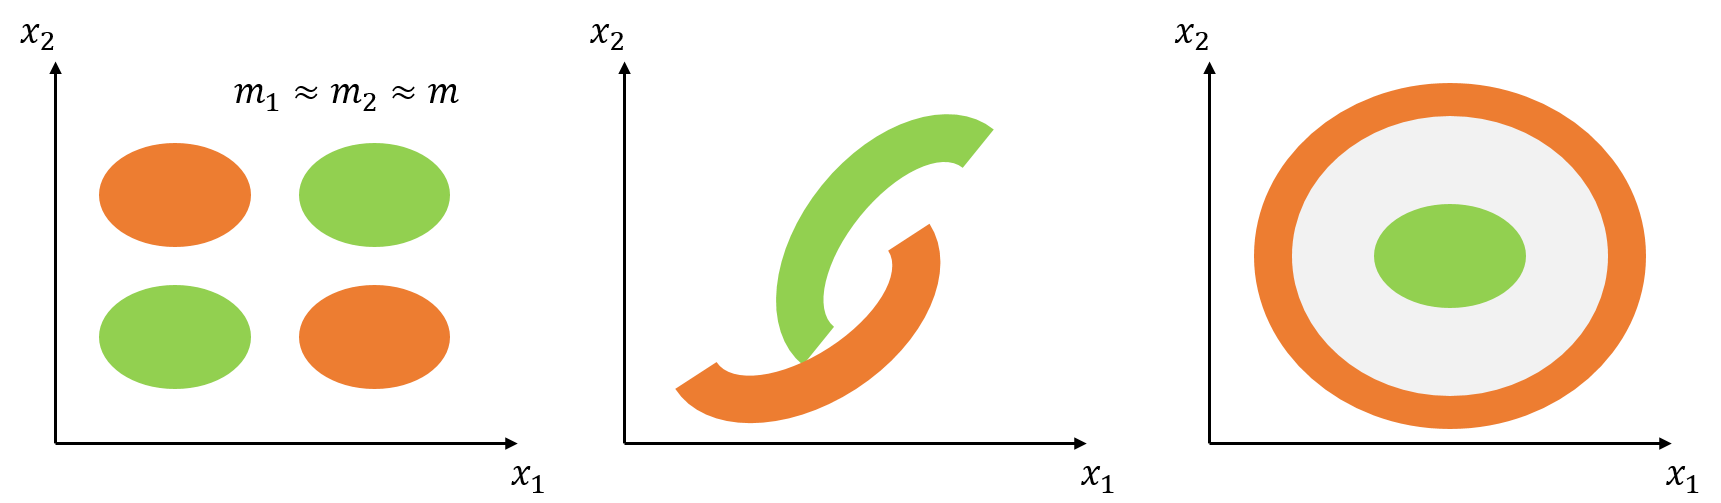
\includegraphics[width=0.9\linewidth]{../figures/statisticalLearning/linearModelClassification/linearDiscriminateComplexStructureDemo}
	\caption{Fisher linear discriminate will fail to achieve class separability for complex data structures.}
	\label{fig:lineardiscriminatecomplexstructuredemo}
\end{figure}



\begin{remark}[rank deficiency for high-dimensional input]
	Another complication in applying LDA and Fisher's discriminant to real data occurs when the number of measurements of each sample (i.e., the dimensionality of each data vector) exceeds the number of samples in each class.[4] In this case, the covariance estimates do not have full rank, and so cannot be inverted. There are a number of ways to deal with this. One is to use a pseudo inverse instead of the usual matrix inverse in the above formula. However, better numeric stability may be achieved by first projecting the problem onto the subspace spanned by $\Sigma_{b}$. Another strategy to deal with small sample size is to use a shrinkage estimator of the covariance matrix, which can be expressed mathematically as
	
	$$\Sigma =(1-\lambda )\Sigma +\lambda I \Sigma =(1-\lambda )\Sigma +\lambda I,$$
	where $I$ is the identity matrix, and $ \lambda $ is the shrinkage intensity or regularisation parameter. This leads to the framework of regularized discriminant analysis or shrinkage discriminant analysis	
	
\end{remark}


\subsection{Multi-dimensional linear discriminate}

\subsubsection{Basics}

\begin{definition}[multi-dimensional linear discriminate]\label{ch:statistical-learning:ch:statistical-learning:th:OptimalityConditionFisherCriterionMultiDimensional}\cite[654]{johnson2007applied}
	Consider a set of input data $x_1,...,x_N\in \R^D$ being classified as two classes such that $y_i\in \{1,2\}$ and the following definition	
	\begin{itemize}
		\item Within-class scatter matrix
		$$S_W = \sum_{i=1}^C \sum_{j:y_j = i} (x_i - \mu_i)(x_i - \mu_i)^T,$$
		where $\mu_i = \frac{1}{N_i}\sum_{j:y_j = i} x_i$.
		\item Between-class scatter matrix
		$$S_B = \sum_{i=1}^C N_i(\mu_i - \mu)(\mu_i - \mu)^T,$$
		where $\mu = \frac{1}{N}\sum_{i=1} x_i = \frac{1}{N}\sum_{i = i}^C N_i\mu_i$.
	\end{itemize}
	
	
	The goal is to seek $w_1,...,w_s\in \R^D$ such that the projection of $x$ onto the subspace spanned by $W=[w_1,...,w_s]$ maximize the separability of the projections $W^Tx_1, W^Tx_2,..., W_Tx_N$. The vectors $w_1,...,w_s$ are known as \textbf{linear discriminants}. 
	
	Or equivalently, the goal is to maximize projected mean distance over total within-class \textbf{projected scattering} via maximizing the following \textbf{Fisher criterion functions}:
	\begin{itemize}
		\item $$J_1(w_1) =\frac{w^T_1S_Bw_1}{w^T_1S_Ww_1},$$
		\item $$J_2(w_2) =\frac{w^T_2S_Bw_2}{w^T_2S_Ww_2}, ~s.t.~ Cov(w_1^TX,w_2^TX) = 0 ,$$
		where $X$ is the data matrix consisting of $x_1,...,x_N$.
		\item
		\begin{align*}
		& J_k(w_k) =\frac{w^T_kS_Bw_k}{w^T_kS_Ww_k},k=3,...,s,\\ 
		~s.t.~ & Cov(w_1^TX,w_k^TX) = 0,\\
		& ... \\
		& Cov(w_{k-1}^TX,w_k^TX). 
		\end{align*}
	\end{itemize}
\end{definition}

\begin{theorem}[discriminants for multi-dimensional LDA]
	The discriminants $w_1,w_2,...,w_s$	are given by $$S_W^{-1/2}u_1,S_W^{-1/2}u_2,...,S_W^{-1/2}u_s$$, where $u_1,u_2,...,u_s$ are the eigenvectors of the matrix $S_W^{-1/2}S_BS_W^{-1/2}$ associated with eigenvalues $\lambda_1\geq \lambda_2 \geq \cdots \geq \lambda_s$.
\end{theorem}
\begin{proof}
	(1) Note that $$Cov(w_1^TX,w_k^TX) = w_1^TCov(X,X)w_k = w_1S_Ww_k,$$
	therefore, the set of maximization problems are the direct result general quadratic form optimization problem in \autoref{ch:linearalgebra:th:MaximizingGeneralizedQuadraticFormsOnUnitSpheres}.
\end{proof}


\subsubsection{Dimensional reduction via LDA}

\begin{method}
	The dimension reduction via LDA has the following steps:
	\begin{itemize}
		\item Compute the mean vectors for each classes
		$$m_i = \frac{1}{N_i}\sum_{j:y_j=i} x_j.$$
		\item Compute the within-class scatter matrix
		$$S_W = \sum_{i=1}^K\sum_{j:y_j=i}  (x_j - m_i)(x_j - m_i)^T.$$
		\item Compute the between-class scatter matrix
		$$S_B = \sum_{i=1}^K N_i (m_i - m)(m_i - m)^T,$$
		where $m$ is the overall mean.
		\item Solve the eigenvalue problem for the matrix $S_W^{-1}S_B$ such that
		$$S_W^{-1}S_B$$
		\item Construct the new low dimensional feature space.
		
	\end{itemize}	
\end{method}


\begin{remark}[eigenvalue properties of the matrix $S_W^{-1}S_B$]
	Let $S_B$ be the between-class scatter matrix of $K$ classes. Then the matrix $S_W^{-1}S_B$ has at most $K-1$ non-zero eigenvalues.
	
	This is because:
	\begin{itemize}
		\item $S_B$ is the sum of $K$ rank 1 matrices like $(\mu_i - \mu)(\mu_i - \mu)^T$; therefore $S_B$ has at most $K$ ranks. And from \autoref{ch:linearalgebra:th:rankOfMatrixProducts}, $$rank(S_W^{-1}S_B)\leq \min(rank(S_W^{-1}),rank(S_B)) = \min(D, K)$$
		\item $S_B$ is a matrix that has been demeaned via projection, i.e., 
		$$S_B = U(I - \frac{1}{K}J)U^T, U = [\mu_1,...,\mu_K]$$
		where $UU^T$ has rank at most $K$. Therefore, $S_B$ has rank at most $K-1$ (use \autoref{ch:linearalgebra:rankPropertyofXTXmatrix}). 
		\item In conclusion, 
		$$rank(S_W^{-1},S_B) = \min(D, K-1).$$
	\end{itemize} 		
\end{remark}



\begin{remark}[PCA vs. LDA]\hfill
	\begin{itemize}
		\item PCA is not optimal for classification task since class label information is not used in searching principal components.
		\item PCA keeps dimensions with largest variance but might throw out dimensions with discriminant information (i.e., class label information).
		\item LDA tries to keep dimensions that contains the most variance between classes using class label information.
	\end{itemize}	
\end{remark}


\begin{example}
	Consider the following classification task on Iris data. 
	
	
\end{example}

\subsubsection{Application in classification}
\begin{lemma}[distance metric in the projected coordinates and variance preserving]
	Let $w_1,w_2,...,w_p$ be the \textbf{complete set} of Fisher linear discriminant and $x\in\R^D$ be a new input such that $w_i = S_W^{-1/2}e_i$, where $e_i$ is the unit eigenvector of $S_W^{-1/2}S_BS_W^{-1/2}$.	It follows that
	\begin{itemize}
		\item The distance of a sample $x$ to its class mean $m_i$ in the projected coordinates is \footnote{Note that the distance to mean via projected coordinates preserves the within-class-scattering weighted distance.} 
		$$d_i(x) =  \norm{y - m_i^{(y)}}^2 = (x-m_1)^TS_W^{-1}(x-m_i)^T, i=1,2,...,K.$$
		where $y = W^Tx, m_i^{(y)} = W^Tm_i.$
		\item Let $\cV$ be the subspace spanned by $V = [w_1,...,w_s]$. Then is the total class-variance in projected coordinates $V^Tx_1,...,V^Tx_N$ is given by
		$$\Delta^2_V = \sum_{i=1}^K (V^Tm_i - V^Tm)^T(V^Tm_i - V^Tm) = \lambda_1 + ... + \lambda_s.$$
		\item Total class variance is related by  
		$$\Delta^2 = \sum_{i=1}^K (m_i - m)^T(m_i - m) = \lambda_1 + ... + \lambda_p.$$
	\end{itemize}	
\end{lemma}
\begin{proof}
	(1) 
	Consider class 1. 
	\begin{align*}
	d_1 &= \norm{W^T(x - m_1)}^2 \\
	&= \sum_{i=1}^p \abs{w_i^T(x-m_1)}^2 \\
	&= \sum_{i=1}^p(x-m_1)^TS_W^{-1/2}e_ie_i^TS_W^{-1/2}(x-m_1) \\
	&= (x-m_1)^TS_W^{-1/2}\sum_{i=1}^p(e_ie_i^T)S_W^{-1/2}(x-m_1) \\
	&= (x-m_1)^TS_W^{-1/2}E^TES_W^{-1/2}(x-m_1) \\
	&= (x-m_1)^TS_W^{-1/2}S_W^{-1/2}(x-m_1) \\
	&= S_W^{-1}(x-m_1) 
	\end{align*}
	(2)(3)	
	\begin{align*}
	\Delta^2_V &= \sum_{i=1}^K (V^Tm_i - V^Tm)^T(V^Tm_i - V^Tm) \\
	&= \sum_{i=1}^K (m_i - m)^TVV^T(m_i - m) \\
	&= Tr(\sum_{i=1}^K (m_i - m)^TVV^T(m_i - m)) \\
	&= Tr(VV^T\sum_{i=1}^K (m_i - m)(m_i - m)^T) \\
	&= Tr(VV^TS_B) \\
	&= \lambda_1 + ... + \lambda_s
	\end{align*}
	
	Note that a similar proof is in \autoref{ch:statistical-learning:th:PCAVariancePreservingProperty}. 
\end{proof}


\begin{remark}[implications and dimensional reduction]
	Using top $s$ discriminants, we can use low-dimensional representation $y_i = V^Tx_i$, which preserves most of the class-variance.
\end{remark}

\section{Logistic regression}


\subsection{Logistic linear model}


\begin{definition}[logistic regression model for $K$ classies]\index{logistic regression}
	Let the training data consists of $N$ pairs $(x_1,y_1),(x_2,y_2),...,(x_N,y_N)$, with $x_i \in \R^{p}, y_i \in \{1,2,...,K\}$. Then the \textbf{logistic model} models the probabilities as
	\begin{align*}
	P(Y = k|X=x) &= \frac{\exp(\beta_{k0} + \beta_k^Tx)}{1 + \sum_{l=1}^{K-1}\exp(\beta_{l0}+\beta_l^Tx)}, k=1,2,...,K-1, \\
	P(Y = K|X=x) &= \frac{1}{1 + \sum_{l=1}^{K-1}\exp(\beta_{l0}+\beta_l^Tx)} \\
	\end{align*}
	where $\beta_{10},\beta_{20},...,\beta_{K0} \in \R$ and vectors $\beta_1,...,\beta_K\in\R^p$ are model parameters.
\end{definition}


\begin{definition}[logistic regression model for two classes]\index{logistic regression}
	Let the training data consists of $N$ pairs $(x_1,y_1),(x_2,y_2),...,(x_N,y_N)$, with $x_i \in \R^{p}, y_i \in \{1,2,...,K\}$. Then the \textbf{logistic model} models the probabilities as
	$$P(Y=1|X=x) = \frac{\exp(\beta_0 + x^T\beta)}{1 + \exp(\beta_0 + x^T\beta)},$$
	and
	$$P(Y=2|X=x) = 1- P(Y=1|X) = \frac{1}{1 + \exp(\beta_0 + x^T\beta)},$$ 
	where $\beta_0 \in \R$ and $\beta\in\R^p$ are model parameters.
\end{definition}


\begin{remark}[probabilities for comparison]\hfill
	\begin{itemize}
		\item For $K$ class classification problem,
		\begin{align*}
		\log \frac{P(Y = i|X=x)}{P(Y = j|X=x)} &= \frac{\beta_{i0} + \beta_i^Tx}{\beta_{j0} + \beta_i^Tx}, i\neq K, j\neq K \\
		\log \frac{P(Y = i|X=x)}{P(Y = K|X=x)} &= \beta_{K0} + \beta_K^Tx, i\neq K \\
		\end{align*}
		\item For binary class classification problem,
		$$\log \frac{P(Y = 1|X=x)}{P(Y = 2|X=x)} = \beta_{0} + \beta^Tx.$$
	\end{itemize}	
\end{remark}


\begin{figure}[H]
	\centering
	\begin{subfigure}[t]{0.45\textwidth}
		\centering
		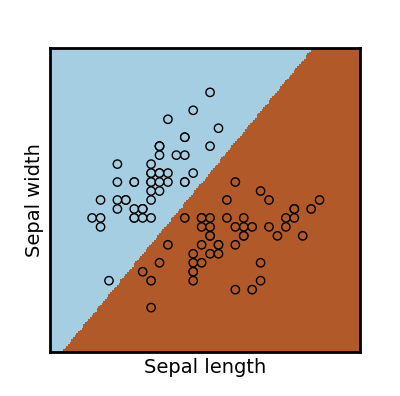
\includegraphics[width=1\linewidth]{../figures/statisticalLearning/linearModelClassification/logisticRegressionIrisDemo1}
		\caption{Decision boundary of a two-class classification problem. The conditional distributions are represented by the contours of the Gaussian distribution.}
	\end{subfigure}\quad
	\begin{subfigure}[t]{0.45\textwidth}
		\centering
		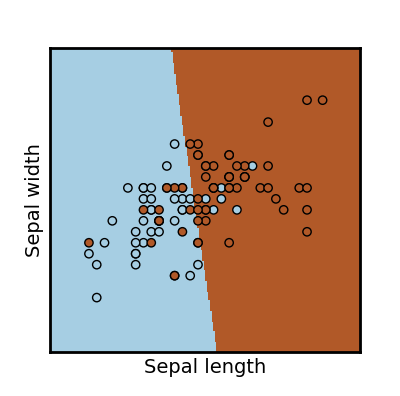
\includegraphics[width=1\linewidth]{../figures/statisticalLearning/linearModelClassification/logisticRegressionIrisDemo2}
		\caption{ A 3D view of the conditional distributions.}
	\end{subfigure}
	\caption{Geometry of decision boundary.}
	\label{fig:linearGaussianDiscriminateModeDecisionBoundaryDemo}
\end{figure}


\subsection{Parameter estimation}
\subsubsection{Maximum likelihood estimation(MLE) for binary classification}

\begin{lemma}[likelihood function, gradient and Hessian for binary logistic regression]\label{ch:statistical-learning:th:LikelihoodFunctionOfLogisticRegression}
	The log-likelihood function for \textbf{binary logistic regression} with $N$ observations is given by
	$$L(\beta) = \sum_{i=1}^{N} (y_i\beta^Tx_i - \log(1 + \exp(\beta^Tx_i))),$$
	where $y_i\in \{0,1\}, x_i\in \R^p,\beta \in \R^p$.	
	
	The gradient and Hessian of the log-likelihood function are given by the following
	\begin{align*}
	g(\beta) &= \frac{d L(\beta)}{d \beta} = \sum\limits_{i=1}^N x_i(y_i - p_i(x_i;\beta))  = X^T(y - p), y\in \R^n, p\in \R^n, X\in \R^{n\times p}.\\
	H(\beta) &= \frac{d g^T(\beta)}{\mathrm{d} \beta}= -\sum_{i=1}^{N} x_ix_i^T p(x_i;\beta)(1-p(x_i;\beta)) = -X^TWX
	\end{align*}
	where $p_i(x_i;\beta)$ is the probability of being 1 for input $x_i$ and parameter $\beta$, $W$ is an $N\times N$ diagonal matrix of weights with 
	$$W_{ii} = p(x_i;\beta)(1 - p(x_i;\beta)),i=1,2,...,N.$$
\end{lemma}
\begin{proof}
	(1)	
	\begin{align*}
	L(\beta) &= \sum_{i=1}^{N}(y_i\log p_i + (1- y_i)\log(1-p_i)) \\
	&=\sum_{i=1}^{N} (y_i\beta^Tx_i - y_i \log(1 + \exp(\beta^T x_i) + (1-y_i)\log 1 - (1-y_i)\log(1 + \exp(\beta^Tx))\\
	&=\sum_{i=1}^{N} (y_i\beta^Tx_i - \log(1 + \exp(\beta^Tx_i)))
	\end{align*}	
	(2)
	\begin{align}
	\vec{g}(\beta) &= \frac{d L(\beta)}{d \beta} \\
	&= \frac{d}{d\beta}(\sum_{i=1}^{N} (y_i\beta^Tx_i - \log(1 + \exp(\beta^Tx_i))))\\
	&=\sum_{i=1}^{N} (y_ix_i - \frac{x_i \exp(\beta^Tx_i)}{1 + \exp(\beta^Tx_i)})\\
	&=\sum_{i=1}^{N} (y_ix_i - x_ip_i) \\
	&= \sum\limits_{i=1}^N x_i(y_i - p_i(x_i;\beta)) \\
	& = X^T(y - p)
	\end{align}
	and
	\begin{align}
	\vec{H}(\beta) &= \frac{d \vec{g}^T(\beta)}{\mathrm{d} \beta} \\
	&=\frac{d}{d\beta} \sum\limits_{i=1}^N x_i(y_i - p_i(x_i;\beta))\\
	&=  \sum\limits_{i=1}^N -x_i(\frac{d}{d\beta} p_i(x_i;\beta))\\
	&=  \sum\limits_{i=1}^N -x_i(x_i^Tp_i - x_i^Tp_i^2)\\
	&= \sum_{i=1}^{N} -x_ix_i^Tp_i(1-p_i) \\
	& = -X^TWX
	\end{align}
\end{proof}



\begin{lemma}[Iteratively reweighted least squares (IRLS) for logistic regression]\cite[250]{murphy2012machine}
	Let $\beta_{old}$ be the current iterate of $\beta$ in maximizing $L(\beta)$ and $W$ be the weighting matrix associated with $\beta_{old}$. Then the Newton-Raphson step is obtained by solving the following optimization problem given by	
	$$\beta^{new} = \arg\min_{\beta}(z-X\beta)^TW(z-X\beta).$$
	where 	$z \triangleq (X\beta^{old} + W^{-1}(y-p))$.
	
	Moreover, the iterative $\beta$ will finally converge since $L(\beta)$ is a concave function.
\end{lemma}
\begin{proof}
	(1)	
	\begin{align*}
	\beta^{new} &= \beta^{old} + (X^TWX)^{-1}X^T(y-p) \\
	&=(X^TWX)^{-1}X^TW(X\beta^{old} + W^{-1}(y-p))\\
	&=(X^TWX)^{-1}X^TWz
	\end{align*}
	where $z \triangleq (X\beta^{old} + W^{-1}(y-p))$.
	(2)The convexity of $L(\beta)$ can be seen from 
	$$H(\beta) = \frac{d g^T(\beta)}{\mathrm{d} \beta} = -X^TWX<0$$
\end{proof}

\begin{algorithm}[H]
	\SetAlgoLined
	\KwIn{Data set consists of $(x_1,y_1),(x_2,y_2),...,(x_N,y_N)$}
	Set $\beta=0$, and compute $p$ by setting its components to
	$$p(x_i;\beta) = \frac{\exp(\beta^Tx_i)}{1 + \exp(\beta^Tx_i)},i=1,2,...,N.$$
	
	Compute the diagonal matrix $W$ with diagonal element being $$W_{ii} = p(x_i;\beta)(1 - p(x_i;\beta)),i=1,2,...,N.$$
	
	\Repeat{stopping criteria is met}{
		$z = X\beta + W^{-1}(y-p)$\\
		$\beta = (X^TWX)^{-1}X^TWz$.
	}
	
	\KwOut{the optimalized value $\beta$.}
	\caption{Iteratively reweighted least squares for logistic regression}
\end{algorithm}


\subsection{Multinomial logistic regression}


\subsubsection{Representation}
\begin{definition}
	\textbf{Multinomial logistic regression} model is also called a \textbf{maximum entropy classifier}, which has the following form
	\begin{align}
	p(y=c|\vec{x},\vec{W}) & =\dfrac{\exp(\vec{w}_c^T\vec{x})}{\sum_{c=1}^C \exp(\vec{w}_c^T\vec{x})}
	\end{align}
\end{definition}

\subsubsection{MLE}
Let $\vec{y}_i=(\mathbb{I}(y_i=1),\mathbb{I}(y_i=1),\cdots, \mathbb{I}(y_i=C))$, $\vec{\mu}_i=(p(y=1|\vec{x}_i,\vec{W}),p(y=2|\vec{x}_i,\vec{W}),\cdots, p(y=C|\vec{x}_i,\vec{W}))$, then the log-likelihood function can be written as
\begin{align}
\ell(\vec{W}) & =\log\prod\limits_{i=1}^N\prod\limits_{c=1}^C \mu_{ic}^{y_{ic}}=\sum\limits_{i=1}^N\sum\limits_{c=1}^C y_{ic}\log \mu_{ic} \\
& = \sum\limits_{i=1}^N\left[\left(\sum\limits_{c=1}^C y_{ic}\vec{w}_c^T\vec{x}_i\right)-\log\left(\sum\limits_{c=1}^C \exp(\vec{w}_c^T\vec{x}_i)\right)\right]
\end{align}

Define the objective function as NLL
\begin{equation}
J(\vec{W})=\mathrm{NLL}(\vec{W})=-\ell(\vec{W})
\end{equation}

Define $\vec{A} \otimes \vec{B}$ be the \textbf{kronecker product} of matrices $\vec{A}$ and $\vec{B}$.If $\vec{A}$ is an $m \times n$ matrix and $\vec{B}$ is a $p \times q$ matrix, then $\vec{A} \otimes \vec{B}$ is the $mp \times nq$ block matrix
\begin{equation}
\vec{A} \otimes \vec{B} \triangle \left(\begin{array}{ccc}
a_{11}\vec{B} & \cdots & a_{1n}\vec{B} \\
\vdots & \vdots & \vdots \\
a_{m1}\vec{B} & \cdots & a_{mn}\vec{B}
\end{array}\right)
\end{equation}

The gradient and Hessian are given by
\begin{align}
\vec{g}(\vec{W}) & =\sum\limits_{i=1}^N (\vec{\mu}-\vec{y}_i) \otimes \vec{x}_i \\
\vec{H}(\vec{W}) & =\sum\limits_{i=1}^N (\mathrm{diag}(\vec{\mu}_i)-\vec{\mu}_i\vec{\mu}_i^T) \otimes (\vec{x}_i\vec{x}_i^T)
\end{align}
where $\vec{y}_i=(\mathbb{I}(y_i=1),\mathbb{I}(y_i=1),\cdots, \mathbb{I}(y_i=C-1))$ and $\vec{\mu}_i=(p(y=1|\vec{x}_i,\vec{W}),p(y=2|\vec{x}_i,\vec{W}),\cdots, p(y=C-1|\vec{x}_i,\vec{W}))$ are column vectors of length $C-1$.

Pass them to any gradient-based optimizer.


\begin{remark}[deriving gradient the Hessian]
	\begin{itemize}
		\item Note that $$l = \sum_{n=1}^{N}\sum_{k=1}^{C}y_{nk}\ln \mu_{nk},$$
		then
		\begin{align*}
		\frac{\Pa l}{\Pa w_j} = & -\sum_{n=1}^{N}\sum_{k=1}^{C}y_{nk}\frac{1}{\mu_{nk}}\frac{\Pa \mu_{nk}}{w_j} \\
		=&-\sum_{n=1}^{N}\sum_{k=1}^{C}y_{nk}\frac{1}{\mu_{nk}}\frac{\exp(w_k^Tx_n)}{(\exp(w_k^Tx_n))^2}(-\exp(w_k^Tx_n)x_n+x_n\delta_{ij}) \\
		=&-\sum_{n=1}^{N}\sum_{k=1}^{C}y_{nk}\frac{1}{\mu_{nk}}\mu_{nk}\mu_{nj}x_n + x_n\delta_{jk}\mu_{nk}
		=&\sum_{n=1}^{N}\sum_{k=1}^{C} (y_{nk}\mu_{nj}x_n + y_{nk}\frac{1}{\mu_{nk}}x_n\delta_{jk})\\
		=&\sum_{n=1}^{N} x_n(\mu_{nj}-y_{nj})
		\end{align*}
	\end{itemize}	
	
\end{remark}



\subsubsection{MAP}
The new objective
\begin{align}
J'(\vec{W}) & =\mathrm{NLL}(\vec{w})-\log{p(\vec{W})} \\
& \quad \text{, where } p(\vec{W}) \triangleq \prod\limits_{c=1}^C \mathcal{N}(\vec{w}_c|\vec{0},\vec{V}_0) \nonumber \\
& = J(\vec{W})+\dfrac{1}{2}\sum\limits_{c=1}^C \vec{w}_c\vec{V}_0^{-1}\vec{w}_c \\
\end{align}

Its gradient and Hessian are given by
\begin{align}
\vec{g}'(\vec{w}) & =\vec{g}(\vec{W})+\vec{V}_0^{-1}\left(\sum\limits_{c=1}^C \vec{w}_c\right) \\
\vec{H}'(\vec{w}) & =\vec{H}(\vec{w})+\vec{I_C} \otimes \vec{V}_0^{-1}
\end{align}

This can be passed to any gradient-based optimizer to find the MAP estimate. Note, however, that the Hessian has size $((CD)×(CD))$, which is $C$ times more row and columns than in the binary case, so limited memory BFGS is more appropriate than Newton’s method.







\subsection{Logistic regression with regularization}
\subsubsection{$L^2$ regularization}
\begin{lemma}[MLE with $L^2$ regularization]
	The maximum likelihood problem for the parameter $\beta$ under $L^2$ regularization is given by \footnote{$\beta_0$ is not penalized.}
	\begin{align*}
	&	\max_{\beta} L_r(\beta,\lambda) \triangleq L(\beta) - \lambda \beta^T\beta \\
	& \max_{\beta} \sum_{i=1}^{N} (y_i\beta^Tx_i - \log(1 + \exp(\beta^Tx_i))) - \lambda \beta^T\beta 
	\end{align*}
	and the gradient and Hessian are given by
	\begin{align}
	g_r(\beta) &= g(\beta)+\lambda\beta \\
	H_r(\beta) &= H(\beta)+\lambda\bm{I}
	\end{align}
	where $L(\beta), g(\beta),$ and $H(\beta)$ are the original likelihood function, gradient and Hessian(\autoref{ch:statistical-learning:th:LikelihoodFunctionOfLogisticRegression}).
\end{lemma}
\begin{proof}
	Directly use linearity of differentiation.
\end{proof}

\begin{remark}[optimization aspect for MLE with regularization]
	We can pass these modified equations into any gradient-based optimizer to find the optimizer.	
\end{remark}

\subsubsection{$L^1$ regularization}
\begin{lemma}[MLE with $L^1$ regularization]
	The maximum likelihood problem for the parameter $\beta$ under $L^1$ regularization is given by \footnote{$\beta_0$ is not penalized.}
	\begin{align*}
	&	\max_{\beta} L_r(\beta,\lambda) \triangleq L(\beta) - \lambda \sum_{j=1}^p \abs{\beta_j} \\
	& \max_{\beta} \sum_{i=1}^{N} (y_i\beta^Tx_i - \log(1 + \exp(\beta^Tx_i))) - \lambda \sum_{j=1}^p \abs{\beta_j}
	\end{align*}
	and the gradient and Hessian are given by
	\begin{align}
	g_r(\beta) &= g(\beta)+\lambda\beta \\
	H_r(\beta) &= H(\beta)+\lambda\bm{I}
	\end{align}
	where $L(\beta), g(\beta),$ and $H(\beta)$ are the original likelihood function, gradient and Hessian(\autoref{ch:statistical-learning:th:LikelihoodFunctionOfLogisticRegression}).
\end{lemma}



\section{Generalized linear model}
See \cite[290]{murphy2012machine}

The linear classification problem:\\
Let the training data consist of $N$ pairs $(x_1,y_1),(x_2,y_2),...,(x_N,y_N)$, with $x_i \in \R^p, y_i \in \{1,-1\}$. 
Perform a classification based on probability given as $$P(y=1|x) = \frac{1}{1 + \exp(-(x^Tw + w_0))}$$


\begin{mdframed}
	Assumptions:
	\begin{itemize}
		\item The data Y1, Y2, ..., Yn are independently distributed
		\item The dependent variable Yi does NOT need to be normally distributed, but it typically assumes a distribution from an exponential family (e.g. binomial, Poisson, multinomial, normal,...)
		\item GLM does NOT assume a linear relationship between the dependent variable and the independent variables, but it does assume linear relationship between the transformed response in terms of the link function and the explanatory variables; e.g., for binary logistic regression logit(π) = w0 + 2X.
		Independent (explanatory) variables can be even the power terms or some other nonlinear transformations of the original independent variables.
		\item Errors need to be independent but NOT normally distributed.
		It uses maximum likelihood estimation (MLE) rather than ordinary least squares (OLS) to estimate the parameters, and thus relies on large-sample approximations.
		\item The homogeneity of variance does NOT need to be satisfied.	
	\end{itemize}
\end{mdframed}


\begin{definition}
	The pdf of output variable $Y$ has a distribution in exponential family, with $EY$ being a linear combinations of input variables $1,x_1,x_2,...,x_n$ ($w^Tx$), passing through a nonlinear function, that is
	$$EY = f(w^Tx)$$
	\begin{itemize}
		\item The mean function is a invertible monotonic function of the linear combination, denoted as $g^{-1}$, such that
		$$EY=\mu = g^{-1}(w^Tx)$$
		\item The inverse of the mean function, $g$, is called the link function.
	\end{itemize}
\end{definition}


\begin{remark}\hfill
	\begin{itemize}
		\item In the logistic regression, the mean function is $$g^{-1} = sigmoid(t) = \frac{1}{1+e^{-t}}$$
		\item Logistic regression can be viewed as $Y$(with sample space $\{0,1\}$), has density of bindary distribution $Y\sim Binary(\mu) = Binary(sigmoid(w^Tx))$. That is
		$$P(Y=1 |x ) =  \frac{1}{1 + \exp(-(x^Tw))}$$ 
	\end{itemize}
\end{remark}

\begin{remark}[linear regression as a trivial generalized linear model]
	The linear regression can be viewed as the mean function is $EY = \mu = g^{-1}(x) = x$ and the density of $Y$ is $Y\sim N(\mu,\sigma^2)$
\end{remark}

\begin{remark}[Poisson regression]
	For Poisson regression, we have
	$$p(y) = \frac{\mu^y}{y!}e^{-\mu}$$
	where $y \in \{0, 1, 2, ... \}$, $EY = \mu = \exp(w^Tx)$, $θ = \log(\mu) = w^Tx$, and $\sigma^2 = 1$.
	where the mean function is $g^{-1}(t) = \exp(t)$, the density of $Y$ is $Y\sim Poisson(\mu)$.	
\end{remark}


\begin{remark}[Extension to multi-class classification]
	For k classes, use k discriminant functions, use 1-vs-all scheme.	
\end{remark}



\section{Support vector machine classifier}


\subsection{Motivation and formulation}


\begin{definition}[The support vector machine classification problem]Let the binary classification training data consist of $N$ pairs $(x_1,y_1),(x_2,y_2),...,(x_N,y_N)$, with $x_i \in \R^p, y_i \in \{1,-1\}$. Assuming training data are linearly separable.\footnote{That is, there exist a hyperplane that can correctly classify all training sample.} 
	
	The SVM classification problem consist of the following two steps:	 
	\begin{itemize}
		\item define a hyperplane by, which gives a classification rule of $$y = sign(x^T\beta + \beta_0)$$
		for training and future data.
		\item The hyperplane we find is such that it has biggest distance from the closest $x$ to the hyperplane, as showed in Figure \autoref{ch:StatisticalLearning-linear-models:fig:SVMOptimalHyperplaneDemo}.   
	\end{itemize}
	The optimization problem is formulated as
	$$\max_{\beta,\beta_0,\norm{\beta} = 1} M$$
	subject to
	$$y_i(x_i^T\beta + \beta_0) \geq M,i=1,2,...,N$$
\end{definition}


\begin{figure}[H]
	\centering
	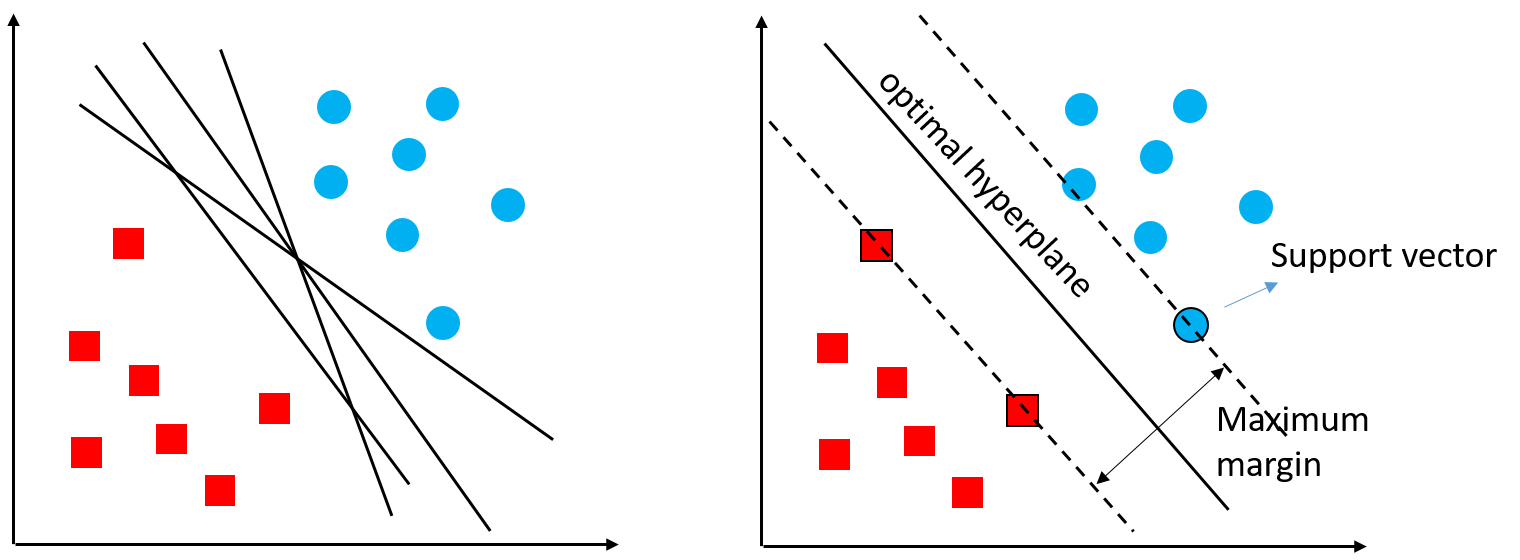
\includegraphics[width=0.9\linewidth]{../figures/statisticalLearning/linearModelClassification/SVMOptimalHyperplaneDemo}
	\caption{}
	\label{ch:StatisticalLearning-linear-models:fig:SVMOptimalHyperplaneDemo}
\end{figure}


\begin{remark}[interpretation]\hfill
	\begin{itemize}
		\item The constraint requires that every point $x$ must be on the correct side(from the multiplier $y_i$), and its distance to the hyperplane has to be at least $M$, with the closest distance to be $M$.
		\item The goal is to maximize the distance from the closest $x$ to the hyperplane.
	\end{itemize}
\end{remark}

\begin{lemma}[reformulation of optimization]
	The optimization problem is formulated as
	$$\max_{\beta,\beta_0,\norm{\beta} = 1} M$$
	subject to
	$$y_i(x_i^T\beta + \beta_0) \geq M,i=1,2,...,N$$
	can be reformulated as
	$$\min_{\beta,\beta_0} \frac{1}{2}\norm{\beta}^2$$
	subject to
	$$y_i(x_i^T\beta + \beta_0) \geq 1,i=1,2,...,N$$
\end{lemma}
\begin{proof}
	In the first formulation, the maximum distance is $M$ such that $y_i(x_i^T\beta + \beta_0) = M$ for some $i$. Let $\beta = 1/M$ in the second formulation, the constraint becomes 
	$$y_i(x_i^T\beta + \beta_0) \geq 1,i=1,2,...,N.$$	
\end{proof}







\begin{lemma}
	Let $f(x) =\{x\in\R^d | w^Tx + b = 0,w\in \R^d,b\in \R\}$ be a hyperplane in $\R^d$, given a point $x_1 \in \R^d$, its signed distance is given as $$(wx_1 + b)/\norm{w}$$
\end{lemma}
\begin{proof}
	Let $x_0 \in \R^d$ be a point on the hyperplane,i.e. $w^Tx_0 + b =0$, then the signed distance is given by projection formula as $w^T(x_1-x_0)/\norm{w} = (w^Tx_1 - w^Tx_0)/\norm{w} = (wx_1 + b)/\norm{w}$.	
\end{proof}

\subsection{Optimality condition and dual form}

\begin{lemma}[KKT condition for primal form]\cite[328]{bishop2006pattern}
	The Lagrangian function is given as
	$$L(w,b,\lambda) = \frac{1}{2}\norm{w}^2 - \sum_{i=1}^N \lambda_i(y_i(x_i^Tw + b) - 1),$$
	with KKT condition as:
	\begin{align*}
	\lambda_i &\geq 0,i=1,...,N \\
	\frac{\Pa L}{\Pa b} = 0 \implies 0 &= \sum_{i=1}^N \lambda_iy_i\\
	\frac{\Pa L}{\Pa w} = 0 \implies w &= \sum_{i=1}^N \lambda_iy_ix_i\\
	\end{align*}
\end{lemma}
\begin{proof}
	See \autoref{ch:constrained-nonlinear-optimization:th:secondorderKKTequalitynecessary}.
\end{proof}


\begin{remark}[conditions for existence of solutions]
	Note that only when data are linearly separable, there are feasible solutions. 	
\end{remark}


\begin{theorem}[dual form optimization problem]
	The dual form of the optimization problem is
	$$\max_{\lambda} \tilde{f}(\lambda) = \sum_{i=1}^N \lambda_i - \frac{1}{2}\sum_{i=1}^N\sum_{j=1}^N \lambda_i\lambda_j y_iy_j x_i\cdot x_j$$
	with constraints:
	\begin{align*}
	\lambda_i &\geq 0, i = 1,...,N\\
	0 &= \sum_{i=1}^N \lambda_iy_i
	\end{align*}
\end{theorem}
\begin{proof}
	Based on the dual problem definition (\autoref{ch:convex-analysis:def:PrimalAndDualProblem}), we have
	$$\tilde{f}(\lambda) = \inf_{w,b} L(w,b,\lambda).$$
	Set first derivatives to zeros, we have
	\begin{align*}
	\frac{\Pa L}{\Pa b} = 0 \implies 0 &= \sum_{i=1}^N \lambda_iy_i\\
	\frac{\Pa L}{\Pa w} = 0 \implies w &= \sum_{i=1}^N \lambda_iy_ix_i
	\end{align*}
	Then
	\begin{align*}
	\tilde{f}(\lambda) &=\frac{1}{2}\sum_{i=1}^N\sum_{j=1}^N \lambda_i\lambda_j y_iy_j x_i\cdot x_j - \sum_{i=1}^N \lambda_i y_i(x_i^Tw)  + \sum_{i=1}^N \lambda_iy_ib + \sum_{i=1}^N \lambda_i\\
	&= -\frac{1}{2}\sum_{i=1}^N\sum_{j=1}^N \lambda_i\lambda_j y_iy_j x_i\cdot x_j + \sum_{i=1}^N \lambda_i
	\end{align*}
	The dual problem constraints are the constraints on the Lagrangian multipliers. 
\end{proof}


\begin{remark}[prediction and support vectors]
	\begin{itemize}
		\item If we replace plug $\beta = \sum_{i=1}^N \lambda_iy_ix_i$ into $y = \beta^Tx + w_0$, we get
		$$y = \sum_{i=1}^N \lambda_i y_ix_i^T x + w_0.$$
		\item \textbf{support vectors are $x_i$ with} $\lambda_i > 0$.
	\end{itemize}
\end{remark}



\begin{remark}[advantages of dual form, link to kernel methods]\hfill
	\begin{itemize}
		\item The dual form involves optimizing over $N$ dual variables, whereas the primal form involves optimization over $D$ variables; the dual form is beneficial when $D\gg N$.
		\item The dual form only requires the inner product between $x_i$ and $x_j$, which can be extended to other kernels using kernel trick.
	\end{itemize}	
\end{remark}

\subsection{Soft margin SVM}
\subsubsection{Basics}
\begin{definition}
	The \textbf{soft margin SVM classification} is formulated as minimization as
	$$\min_{w,b,\eta} \frac{1}{2}\norm{w}^2 + C\sum_{i=1}^n \eta_i$$
	under the constraints:
	\begin{align*}
	y_i(x_i^Tw + b) &\geq 1 - \eta_i,i=1,2,...,N\\
	\eta_i &\geq 0, i=1,...,N
	\end{align*}
	where the $C$ is the regulation parameter.  
\end{definition}

\begin{remark}[interpret regularization parameter]\hfill
	\begin{itemize}
		\item When $C\to \infty$, the soft margin optimization problem will converge to the hard margin SVM.
		\item $C$ is a regularization parameter that controls the trade-off between maximizing the margin and minimizing the training error. Small $C$ tends to emphasize the margin while ignoring the outliers in the training data, while large $C$ may tend to overfit the training data.
	\end{itemize}	
\end{remark}



\begin{figure}[H]
	\centering
	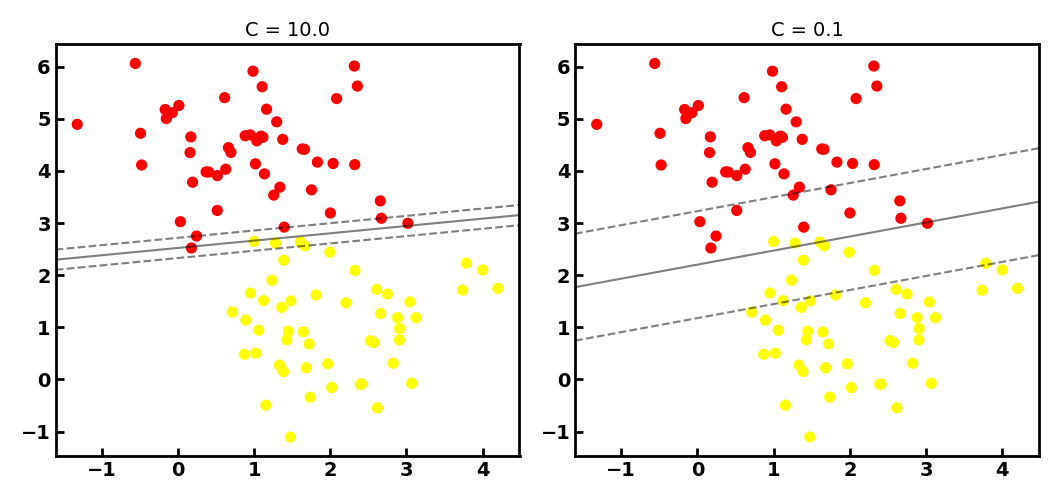
\includegraphics[width=0.7\linewidth]{../figures/statisticalLearning/linearModelClassification/softSVMClassificationExample}
	\caption{}
	\label{fig:softsvmclassificationexample}
\end{figure}





\subsubsection{Optimality condition*}

\begin{lemma}[KKT condition for primal form]\cite[332]{bishop2006pattern}
	The Lagrangian function is given as
	$$L(w,w_0,\eta,\lambda, \mu) = \frac{1}{2}\norm{w}^2 + C\sum_{i=1}^N \eta_i - \sum_{i=1}^N \lambda_i(y_i(x_i^Tw + w_0) - 1) - \sum_{i=1}^N \mu_i\eta_i,$$
	with KKT condition as:
	\begin{align*}
	\lambda_i &\geq 0,i=1,...,N ~(dual~ feasible)\\
	\mu_i &\geq 0,i=1,...,N ~(dual~feasible)\\
	y_i(x_i^Tw + w_0) &\geq 1 - \eta_i,i=1,2,...,N ~(primal~feasible)\\
	\eta_i &\geq 0, i=1,...,N ~(primal~feasible)\\
	\lambda_i(y_i(x_i^Tw + w_0) - 1 + \eta_i) &= 0,i=1,2,...,N ~(complementrary~slackness)\\
	\frac{\Pa L}{\Pa w_0} = 0 \implies 0 &= \sum_{i=1}^N \lambda_iy_i\\
	\frac{\Pa L}{\Pa w} = 0 \implies w &= \sum_{i=1}^N \lambda_iy_ix_i\\
	\frac{\Pa L}{\Pa \eta_i} = 0 \implies 0 &= C-\lambda_i-\mu_i, i=1,2,...,N.
	\end{align*}
\end{lemma}
\begin{proof}
	See \autoref{ch:constrained-nonlinear-optimization:th:secondorderKKTequalitynecessary}.
\end{proof}

\begin{theorem}[dual form optimization problem]\cite[333]{bishop2006pattern}
	The dual form of the optimization problem is
	$$\max_{\lambda}\tilde{L}(\lambda) = \sum_{i=1}^N \lambda_i - \frac{1}{2}\sum_{i=1}^N\sum_{j=1}^N \lambda_i\lambda_j y_iy_j x_i^Tx_j$$
	with constraints:
	\begin{align*}
	C\geq \lambda_i &\geq 0, i = 1,...,N\\
	0 &= \sum_{i=1}^N \lambda_iy_i
	\end{align*}
\end{theorem}
\begin{proof}
	Based on the dual problem definition (\autoref{ch:convex-analysis:def:PrimalAndDualProblem}), we have
	$$\tilde{f}(\lambda, \mu) = \inf_{w,b} L(w,b,\eta,\lambda,\mu).$$
	Set first derivatives to zeros, we have
	\begin{align*}
	\frac{\Pa L}{\Pa b} = 0 \implies 0 &= \sum_{i=1}^N \lambda_iy_i\\
	\frac{\Pa L}{\Pa w} = 0 \implies w &= \sum_{i=1}^N \lambda_iy_ix_i \\
	\frac{\Pa L}{\Pa \eta_i} = 0 \implies 0 &= C-\lambda_i-\mu_i, i=1,2,...,N.
	\end{align*}
	Then
	\begin{align*}
	\tilde{L}(\lambda,\mu) &=\frac{1}{2}\sum_{i=1}^N\sum_{j=1}^N \lambda_i\lambda_j y_iy_j x_i\cdot x_j - \sum_{i=1}^N \lambda_i y_i(x_i^Tw)  + \sum_{i=1}^N \lambda_iy_ib + \sum_{i=1}^N \lambda_i + \sum_{i=1}^N \eta_i (C - \lambda_i-\mu_i)\\
	&= -\frac{1}{2}\sum_{i=1}^N\sum_{j=1}^N \lambda_i\lambda_j y_iy_j x_i\cdot x_j + \sum_{i=1}^N \lambda_i
	\end{align*}
	The dual problem constraints are the constraints on the Lagrangian multipliers. In summary, we have
	$$\tilde{L}(\lambda) = \sum_{i=1}^N \lambda_i - \frac{1}{2}\sum_{i=1}^N\sum_{j=1}^N \lambda_i\lambda_j y_iy_j x_i^Tx_j$$
	with constraints:
	\begin{align*}
	\lambda_i &\geq 0, i = 1,...,N\\
	\mu_i &\geq 0, i = 1,...,N\\
	C &= \lambda_i + \mu_i , i = 1,...,N\\
	0 &= \sum_{i=1}^N \lambda_iy_i.
	\end{align*}
	Note that the first three conditions can be simplified to 
	$$0\leq \lambda_i\leq C, i =1,2...,N.$$
\end{proof}

\subsubsection{Algorithm}


\begin{algorithm}[H]
	\SetAlgoLined
	\KwIn{Training data $(x_1,y_1),...,(x_N,y_N)$ where $x_i\in X$, $y_i\in Y = \{-1,1\}$}
	Initialize regularizer parameter $C>0$ and construct the dual form convex optimization problem:
	\begin{align*}
	& \min_{\lambda} \frac{1}{2}\sum_{i=1}^N\sum_{j=1}^N \lambda_i\lambda_j y_iy_j(x_i\cdot x_j) - \sum_{i=1}^N \lambda_i \\
	s.t. &  \sum_{i=1}^N \lambda_i y_i = 0\\
	& 0 \leq \lambda_i \leq C, i=1,2,...,N
	\end{align*}\\
	Solve the optimization problem $\lambda^*=(\lambda_1^*,...,\lambda_N^*)$.\\
	Compute $w^* = \sum_{i=1}^N \lambda_i^* y_ix_i$ based on KKT condition.\\
	Select \textbf{any} $\lambda_i^*$ satisfying $0<\lambda_i^*<C$, and compute
	$$b^* = y_i - \sum_{i=1}^N y_i \lambda_i^* (x_i\cdot x_j).$$
	
	Compute the separating hyperplane via
	$$x^Tw^* + b^* = 0.$$
	
	Get the decision function
	$$f(x) = sign(x^Tw^* + b^*)$$
	
	\KwOut{$f(x)$}
	\caption{Soft margin SVM algorithm}
\end{algorithm}


\begin{remark}[the value of $b^*$]
	From the KKT condition that if $\lambda_i$ is not binding to the constraints $0$ and $C$, i.e., $0<\lambda_i<C$, then the constraint $	y_i(x_i^Tw + b^*) = 1$ is satisfied.
	
	Therefore, we have
	\begin{align*}
	y_i(x_i^Tw + w_0) = 1 \\
	b^* = \frac{1}{y_i} - x_i^Tw^* \\
	b^* = y_i - x_i^Tw^* \\
	b^* = y_i - \sum_{i=1}^N y_i \lambda_i^* (x_i\cdot x_j) 
	\end{align*}
	
	Note that $b^*$ is not necessarily unique.	In reality, we can take the average vlaue of all qualified $b^*$.
\end{remark}


\subsection{SVM with kernels}
\subsubsection{Basics}
\begin{lemma}[Kernel SVM problems]\cite[333]{bishop2006pattern}
	The dual form of the optimization problem is
	$$\tilde{L}(\lambda) = \sum_{i=1}^N \lambda_i - \frac{1}{2}\sum_{i=1}^N\sum_{j=1}^N \lambda_i\lambda_j y_iy_j k(x_i,x_j)$$
	with constraints:
	\begin{align*}
	C\geq \lambda_i &\geq 0, i = 1,...,N\\
	0 &= \sum_{i=1}^N \lambda_iy_i
	\end{align*}
\end{lemma}
\begin{proof}
	Directly substitute the constraints in the primal form.
\end{proof}

Classifier:
$$f(x) = \sum_{i=1}^N \lambda_i y_i k(x_i,x) + b.$$


\subsubsection{Algorithms}
\begin{algorithm}[H]
	\SetAlgoLined
	\KwIn{Training data $(x_1,y_1),...,(x_N,y_N)$ where $x_i\in X$, $y_i\in Y = \{-1,1\}$}
	Initialize regularizer parameter $C>0$, select a kernel $k(x_1,x_2)$, and construct the dual form convex optimization problem:
	\begin{align*}
	& \min_{\lambda} \frac{1}{2}\sum_{i=1}^N\sum_{j=1}^N \lambda_i\lambda_j y_iy_j(x_i\cdot x_j) - \sum_{i=1}^N \lambda_i \\
	s.t. &  \sum_{i=1}^N \lambda_i y_i = 0\\
	& 0 \leq \lambda_i \leq C, i=1,2,...,N
	\end{align*}\\
	Solve the optimization problem $\lambda^*=(\lambda_1^*,...,\lambda_N^*)$.\\
	Compute $w^* = \sum_{i=1}^N \lambda_i^* y_ix_i$ based on KKT condition.\\
	Select \textbf{any} $\lambda_i^*$ satisfying $0<\lambda_i^*<C$, and compute
	$$b^* = y_i - \sum_{i=1}^N y_i \lambda_i^* (x_i\cdot x_j).$$
	
	Compute the separating hyperplane via
	$$x^Tw^* + b^* = 0.$$
	
	Get the decision function
	$$f(x) = sign(x^Tw^* + b^*)$$
	
	\KwOut{$f(x)$}
	\caption{Soft margin SVM algorithm}
\end{algorithm}


\begin{figure}[H]
	\centering
	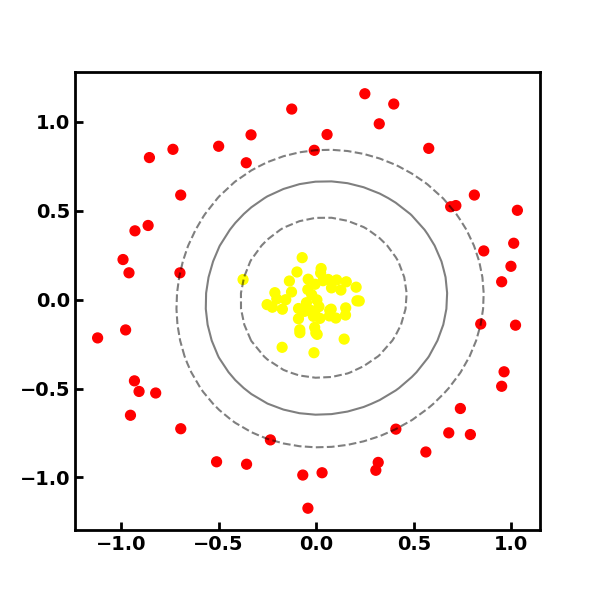
\includegraphics[width=0.5\linewidth]{../figures/statisticalLearning/linearModelClassification/SVMKernelClassificationExample}
	\caption{SVM classification using Gaussian kernel. The original problem cannot be separated by linear kernel.}
	\label{fig:svmkernelclassificationexample}
\end{figure}




\subsection{Compare with logistic regression}


\begin{remark}[Comparison between logistic regression and SVM]
	There are 2 differences to note:
	
	Logistic loss diverges faster than hinge loss. So, in general, it will be more sensitive to outliers.
	Logistic loss does not go to zero even if the point is classified sufficiently confidently. This might lead to minor degradation in accuracy.
	So, you can typically expect SVM to perform marginally better than logistic regression.
	
	
	
	SVM try to maximize the margin between the closest support vectors while LR the posterior class probability. Thus, SVM find a solution which is as fare as possible for the two categories while LR has not this property.
	
	LR is more sensitive to outliers than SVM because the cost function of LR diverges faster than those of SVM. So putting an outlier on above picture would give below picture:
	
	Logistic Regression produces probabilistic values while SVM produces 1 or 0. So in a few words LR makes not absolute prediction and it does not assume data is enough to give a final decision. This maybe be good property when what we want is an estimation or we do not have high confidence into data.	
\end{remark}


\section{Note on bibliography}



\printbibliography
\end{refsection}

\begin{refsection}
\startcontents[chapters]
	\chapter{Generative models}\label{ch:statistical-learning:sec:GenerativeModels}
	%\minitoc
	\printcontents[chapters]{}{1}{}

\section{Generative model for discrete data}

\section{Foundations of Bayesian concept learning}
Psychological research has shown that people can learn concepts from positive examples alone (Xu and Tenenbaum 2007).

We can think of learning the meaning of a word as equivalent to \textbf{concept learning}, which in turn is equivalent to binary classification. To see this, define $f(\vec{x})=1$ if x is an example of the concept $C$, and $f(\vec{x})=0$ otherwise. Then the goal is to learn the indicator function $f$, which just defines which elements are in the set $C$.


\subsection{Likelihood}
\begin{equation}
p(\mathcal{D}|h) \triangleq \left(\dfrac{1}{\text{size}(h)}\right)^N=\left(\dfrac{1}{|h|}\right)^N
\end{equation}

This crucial equation embodies what Tenenbaum calls the \textbf{size principle}, which means the model favours the simplest (smallest) hypothesis consistent with the data. This is more commonly known as \textbf{Occam’s razor}\footnote{\url{http://en.wikipedia.org/wiki/Occam\%27s_razor}}.


\subsection{Prior}
The prior is decided by human, not machines, so it is subjective. The subjectivity of the prior is controversial. For example, that a child and a math professor will reach different answers. In fact, they presumably not only have different priors, but also different hypothesis spaces. However, we can finesse that by defining the hypothesis space of the child and the math professor to be the same, and then setting the child’s prior weight to be zero on certain “advanced” concepts. Thus there is no sharp distinction between the prior and the hypothesis space.

However, the prior is the mechanism by which background knowledge can be brought to bear on a problem. Without this, rapid learning (i.e., from small samples sizes) is impossible.


\subsection{Posterior}
The posterior is simply the likelihood times the prior, normalized.
\begin{equation}
p(h|\mathcal{D}) \triangleq \dfrac{p(\mathcal{D}|h)p(h)}{\sum_{h' \in \mathcal{H}}p(\mathcal{D}|h')p(h')}=\dfrac{\mathbb{I}(\mathcal{D} \in h)p(h)}{\sum_{h' \in \mathcal{H}}\mathbb{I}(\mathcal{D} \in h')p(h')}
\end{equation}
where $\mathbb{I}(\mathcal{D} \in h)p(h)$ is 1 \textbf{iff}(iff and only if) all the data are in the extension of the hypothesis $h$.

In general, when we have enough data, the posterior $p(h|\mathcal{D})$ becomes peaked on a single concept, namely the MAP estimate, i.e.,
\begin{equation}
p(h|\mathcal{D}) \rightarrow \hat{h}^{MAP}
\end{equation}
where $\hat{h}^{MAP}$ is the posterior mode,
\begin{equation}\begin{split}
\hat{h}^{MAP} & \triangleq \arg\max\limits_h p(h|\mathcal{D})=\arg\max\limits_h p(\mathcal{D}|h)p(h) \\
& =\arg\max\limits_h [\log p(\mathcal{D}|h) + \log p(h)]
\end{split}\end{equation}

Since the likelihood term depends exponentially on $N$, and the prior stays constant, as we get more and more data, the MAP estimate converges towards the \textbf{maximum likelihood estimate} or \textbf{MLE}:
\begin{equation}
\hat{h}^{MLE} \triangleq \arg\max\limits_h p(\mathcal{D}|h)=\arg\max\limits_h \log p(\mathcal{D}|h)
\end{equation}

In other words, if we have enough data, we see that the \textbf{data overwhelms the prior}.


\subsection{Posterior predictive distribution}
The concept of \textbf{posterior predictive distribution}\footnote{\url{http://en.wikipedia.org/wiki/Posterior_predictive_distribution}} is normally used in a Bayesian context, where it makes use of the entire posterior distribution of the parameters given the observed data to yield a probability distribution over an interval rather than simply a point estimate. 
\begin{equation}
p(\tilde{\vec{x}}|\mathcal{D}) \triangleq \mathbb{E}_{h|\mathcal{D}}[p(\tilde{\vec{x}}|h)] = \begin{cases}
\sum_h p(\tilde{\vec{x}}|h)p(h|\mathcal{D}) \\
\int p(\tilde{\vec{x}}|h)p(h|\mathcal{D})\mathrm{d}h
\end{cases}
\end{equation}

This is just a weighted average of the predictions of each individual hypothesis and is called \textbf{Bayes model averaging}(Hoeting et al. 1999). 


\section{Beta-binomial model}

\subsection{The model}
\begin{definition}[Beta-binomial model]
A Beta-binomial model with pre-specified parameter $n$ has parameter $a$ and $b$, and can be represented by the following Hierachical model 
$$Y|\theta \sim Binom(n,\theta), \theta\sim Beta(a,b).$$
In particular, 
 the density functions for $Y|\theta$ and $\theta$ given by 
	$$Pr_{Y|\theta}(Y = y|\theta) = \binom{n}{y} \theta^y(1-\theta)^{(n-y)}, y=0,1,...,n;$$
	$$f(\theta) = \frac{1}{B(a,b)}\theta^{a-1}(1-\theta)^{b-1},a>0,b>0;$$
where $$B(a,b) = \int_0^1 \theta^{a-1}(1-\theta)^{b-1} d\theta.$$
\end{definition}



\begin{lemma}[density functions for Beta-binomial model]
Let $(Y,\theta)$ follow  a Beta-binomial model with parameter $(a,b)$, we have
\begin{itemize}
	\item the joint density function is given by
	$$Pr_{Y, \theta}(Y = y, \theta) = \binom{n}{y} \theta^y(1-\theta)^{(n-y)}\frac{1}{B(a,b)}\theta^{a-1}(1-\theta)^{b-1}, y=0,1,...,n;$$
	\item the marginal density function for $y$ is given by
	$$Pr_Y(Y=y)=\binom{n}{y} \frac{B(y+a,n-y+b)}{B(a,b)}.$$
\end{itemize}	
where $$B(a,b) = \int_0^1 \theta^{a-1}(1-\theta)^{b-1} d\theta.$$
\end{lemma}
\begin{proof}
(1) the joint density function is given by
$$Pr_{Y, \theta}(Y = y, \theta) = \binom{n}{y} \theta^y(1-\theta)^{(n-y)}\frac{1}{B(a,b)}\theta^{a-1}(1-\theta)^{b-1}, y=0,1,...,n;$$
(2)the marginal density function for $y$ is given by
$$Pr_Y(Y=y)=\binom{n}{y} \frac{B(y+a,n-y+b)}{B(a,b)}.$$	
\end{proof}





\begin{lemma}[basic statistical properties of Beta-binomial model]\label{ch:statistical-learning:th:BasicStatisticalPropertiesOfBetaBinomialModel}
Let $(Y,\theta)$ follow a Beta-binomial model with parameter $(a,b)$, we have
\begin{itemize}
	\item $$E[Y|\theta] = n\theta, E[\theta] = \frac{a}{a+b}, E[Y] = n\frac{a}{a+b}.$$
	\item $$Var[Y|\theta] = n\theta(1-\theta), Var[Y] = n\mu_{\theta}(1-\mu_\theta)(1 + (n-1)\frac{1}{a+b+1}),$$
	where $\mu_\theta = a/(a+b)$.
\end{itemize}	
\end{lemma}
\begin{proof}
(1) $$E[Y] = E[E[Y|\theta]] = E[n\theta] = nE[\theta] = n\frac{a}{a+b}.$$
(2) Note that 
\begin{align*}
Var[Y] &= E[Var[Y|\theta]] + Var[E[Y|\theta]] \\
&= E[n\theta(1-\theta)] + Var[n\theta] \\
&= E[n\theta] - nE[\theta^2] + n^2 Var[\theta] \\
&= n(E[\theta] - E[\theta]^2 + nVar[\theta]) ]
\end{align*}
where we use the property of conditional variance(\autoref{ch:theory-of-probability:th:conditionalVarianceIdentity}).
then we use the following facts(\autoref{ch:theory-of-statistics:th:propertyBetaDistribution}),
\begin{itemize}
	\item $$E[\theta] = \frac{a}{a+b}.$$
	\item $$E[\theta^2] = \frac{a(a+1)}{(a+b)(a+b+1)}$$
	\item $$Var[\theta] = \frac{ab}{(a+b)^2(a+b+1)}.$$
\end{itemize}
\end{proof}


\subsection{Parameter inference}

\begin{theorem}[posterior distribution and estimation of $\theta$]\cite[75]{murphy2012machine}\label{ch:statistical-learning:th:PosteriorDistributionAndEstimationInBetaBionomialModel}
Given an iid random experiment data set $\cD$ consisting of $N_1$ results of labeling 1 and $N_0$ results of the labeling 0. Consider a Beta-binomial model with parameter $(a,b)$. It follows that
\begin{itemize}
	\item The posterior distribution of parameter $\theta$ given the data $\cD$ is
	$$\theta|\cD \sim Beta(N_1+a,N_0+b),$$
	that is
	$$f_{\theta|\cD} = \frac{1}{B(a+N_1,b+N_0)}\theta^{a+N_1-1}(1-\theta)^{b+N_0-1}.$$
	\item The mean and variance of the posterior $\theta$ is given by
	$$E[\theta|\cD] = \frac{a + N_1}{a + b + N_1 + N_0},$$
	$$Var[\theta|\cD] = \frac{(a + N_1)(b + N_0)}{(a + N_1 + b + N_0)^2(a+b+1 + N_1 + N_0)},$$
	\item The maximum likelihood function is given by
	$$L(\cD|\theta) \propto \theta^{N_1}(1-\theta)^{N_0}  $$
	and the maximum likelihood estimation of $\theta$ is given by
	$$\theta_{MLE} = \frac{N_1}{ N_1 + N_0 }.$$
	\item The maximum a posterior estimation of $\theta$ is given by
	 $$\theta_{MAP} = \frac{a+ N_1 - 1}{a + b + N_1 + N_0 -2},$$
	 when $a = b = 1$, $\theta_{MAP} = \theta_{MLE}.$
\end{itemize} 	
\end{theorem}
\begin{proof}
(1)
Note that
\begin{align*}
p(\theta|\cD) &\propto p(\cD|\theta)p(\theta) \\
 &\propto \theta^{N_1}(1-\theta)^{N_0}\theta^{a-1}(1-\theta)^{b-1} \\
 &=\theta^{N_1+a-1}(1-\theta)^{N_0+b-1} 
\end{align*}
After normalization, we can show $\theta|\cD$ follows $Beta(N_1+a,N_0+b)$.
(2)\autoref{ch:theory-of-statistics:th:propertyBetaDistribution}.
(3)(4)\autoref{ch:theory-of-statistics:th:propertyBetaDistribution}.
\end{proof}

\begin{lemma}[sequential learning property]
Suppose we have two data sets $\cD_1$ and $\cD_2$ with sufficient statistics $N_1',N_0'$ and $N_1'', N_0''$. And denote $N_1 = N_1' + N_1''$ and $N_0 = N_0' + N_0''$.
In batch mode, we have
$$p(\theta|\cD',\cD'') \propto Beta(\theta|N_1+a,N_0 + b).$$
and in sequential mode, we also have
$$p(\theta|\cD',\cD'') \propto Beta(\theta|N_1+a,N_0 + b).$$ 	
\end{lemma}
\begin{proof}
Use \autoref{ch:statistical-learning:th:PosteriorDistributionAndEstimationInBetaBionomialModel}, we have
\begin{align*}
p(\theta|\cD',\cD'') &\propto p(\cD''|\theta)p(\theta|\cD') \\
&\propto Bin(N_1''|\theta,N_1''+N_0'')Beta(\theta|N_1'+a,N_0'+b) \\
&\propto Bin(\theta| N_1'+ N_2'' + a,N_0'+N_0''+b) \\
=Beta(N_1+ a, N_0+b) 
\end{align*}
where we used the conditional Bayesian law(\autoref{ch:theory-of-probability:th:BayesianLawForRandomVariables}).
\end{proof}

\subsection{Forecasting}

\begin{lemma}[posterior prediction for future outcomes]\cite[80]{murphy2012machine}
Suppose we have observations of data set $\cD$ with sufficient statistic $N_1$ and $N_0$. Now for the new $M$ experiments, the number of results with label 1, denoted by random variable $Y$, has the following prediction.
\begin{itemize}
	\item It follows the Beta-binomial model 
	$$Y|\theta \sim Binom(M,\theta), \theta\sim Beta(N_1+a,N_0+b).$$
	In particular, 
	the density functions for $Y|\theta$ and $\theta$ given by 
	$$Pr_{Y|\theta}(Y = y|\theta) = \binom{M}{y} \theta^y(1-\theta)^{(M-y)}, y=0,1,...,M;$$
	$$f(\theta) = \frac{1}{B(N_1+a,N_0 + b)}\theta^{N_1+a-1}(1-\theta)^{N_0+b-1},a>0,b>0;$$
	where $$B(N_1+a,N_0 + b) = \int_0^1 \theta^{N_1+a-1}(1-\theta)^{N_0+ b-1} d\theta.$$
	\item 
	\begin{align*}
	P(Y=y|\cD,M) &= \binom{M}{y}\frac{1}{B(N_1+a,N_0+b)}\int_0^1 \theta^y(1-\theta)^{M-y}\theta^{N_1+a-1}(1-\theta)^{N_0+b-1}\\
	& = \binom{M}{y}\frac{B(N_1+a+y,N_0+b+M-y)}{B(N_1+a,N_0+b)}.
	\end{align*}
	\item the posterior prediction for $Y$ has mean and variance given by
		 $$E[Y] = M\theta,Var[Y|\theta] = n\theta(1-\theta),$$
		 where $\theta = \frac{a+N_1}{a+b+N_1+N_0}$.
\end{itemize}
\end{lemma}
\begin{proof}
(1)Directly from \autoref{ch:statistical-learning:th:BasicStatisticalPropertiesOfBetaBinomialModel}.
(2) Use
$$P(Y|\cD,M)= P(Y|\theta,M) P(\theta|\cD).$$
\end{proof}


\section{Dirichlet-multinomial model}
\subsection{The model}
\begin{definition}[Dirichlet-multinomial model]
	A Dirichlet-multinomial model with pre-specified parameter $N$(total counts) and $K$(number of classes) has parameters $\alpha = (\alpha_1,\alpha_2,...,\alpha_K)$, and can be represented by the following Hierachical model 
	$$Y|\theta \sim Mulnom(n,\theta), \theta\sim Dir(\theta).$$
	In particular, 
	the density functions for $Y|\theta$ and $\theta$ given by 
	$$Pr_{Y|\theta}(Y = (n_1,n_2,...,n_K)|\theta) = \dbinom{N}{n_1\cdots n_K} \theta^y(1-\theta)^{(n-y)}, y=0,1,...,n;$$
	$$f(\theta|\alpha)=Dir(\theta|\alpha) = \dfrac{1}{B(\alpha)}\prod_{k=1}^K \theta_k^{\alpha_k-1}$$
	with support $\theta\in \{\theta_k:0\leq \theta_k\leq 1,\sum_k x_\theta = 1,\forall k=1,2...,K\}$, and $B(a)$ is a normalization constant given as
	$$B(a) = \frac{\prod_{k=1}^K \Gamma(a_k)}{\Gamma(\sum_k a_k)},$$
	where $\Gamma(\cdot)$ is the Gamma function. 
\end{definition}

\begin{example}
Consider tossing a tie with 6 faces. The count on the each distinct faces from a total number count $N$ can be modeled by the Dirichlet-multinomial model.	
\end{example}

\begin{lemma}[density functions for Dirichlet-Multinomial model]
	Let $(Y,\theta)$ follow  a Beta-binomial model with parameter $(a,b)$, we have
	\begin{itemize}
		\item the joint density function  for $(Y,\theta)$ with parameter $\alpha$ is given by
		\begin{align*}
		Pr_{Y, \theta}(Y = (y_1,y_2,...,y_K), \theta) &= \dbinom{N}{N_1\cdots N_K}\prod_{k=1}^K \theta_k^{\alpha_k+y_k-1} \frac{1}{B(\alpha)}\\
		&=\prod_{k=1}^K \theta_k^{\alpha_k+y_k-1} \frac{1}{B(\alpha')}
		\end{align*}
		where $\alpha'=\alpha+(y_1,y_2,...,y_K).$
		\item the marginal density function for $Y_i$ with parameter $\alpha$ is given by
		$$Pr_Y(Y_i=y)=\binom{N}{y_i} \frac{B(y+\theta_i,N-y+(\alpha_0-\alpha_i))}{B(\alpha_i,\alpha_0-\alpha_i)}.$$
	\end{itemize}	
	where $$B(a,b) = \int_0^1 x^{a-1}(1-x)^{b-1} dx.$$
\end{lemma}
\begin{proof}
	(1) the joint density function is given by
	$$Pr_{Y, \theta}(Y,\theta) = Pr(Y|\theta)f(\theta).$$
	(2)the marginal density function for $y$ is given by
	$$Pr_Y(Y=y)=\binom{n}{y} \frac{B(y+a,n-y+b)}{B(a,b)}.$$	
\end{proof}


\begin{remark}[connections between Dirichlet-multinomial model and Beta-binomial model]
In the Dirichlet-multinomial model, we have multiple classes. However, if we are only interested in the counts in one particular class(i.e., the marginal distribution of one types of result), we can convert it to an equivalent Beta-binomial model. 	
\end{remark}


\begin{lemma}[basic statistical properties of Dirichlet-Multinomial model]\label{ch:statistical-learning:th:BasicStatisticalPropertiesOfDirichletMultinomialModel}
	Let $(Y,\alpha),Y=(Y_1,Y_2,...,Y_K),\alpha=(\alpha_1,...,\alpha_K)$ follow a Dirichlet-Multinomial model with parameter $\alpha$. Further denote $\alpha_0=\sum_{i=1}^{K}\alpha_i=1$. Then we have
	\begin{itemize}
		\item $$E[Y_i|\alpha] = N\alpha_i, E[\alpha_i] = \frac{\alpha_i}{\alpha_0}, E[Y] = n\frac{a}{a+b}.$$
		\item $$Var[Y|\theta] = n\theta(1-\theta), Var[Y] = n\mu_{\theta}(1-\mu_\theta)(1 + (n-1)\frac{1}{a+b+1}),$$
		where $\mu_\theta = a/(a+b)$.
	\end{itemize}	
\end{lemma}
\begin{proof}
	(1) $$E[Y_i] = E[E[Y_i|\theta_i]] = E[N\theta_i] = NE[\theta_i] = N\frac{\alpha_i}{\alpha_0}.$$ 
	(2) Note that 
	\begin{align*}
	Var[Y] &= E[Var[Y|\theta]] + Var[E[Y|\theta]] \\
	&= E[n\theta(1-\theta)] + Var[n\theta] \\
	&= E[n\theta] - nE[\theta^2] + n^2 Var[\theta] \\
	&= n(E[\theta] - E[\theta]^2 + nVar[\theta]) ]
	\end{align*}
	where we use the property of conditional variance(\autoref{ch:theory-of-probability:th:conditionalVarianceIdentity}).
	then we use the following facts(\autoref{ch:theory-of-statistics:th:propertyBetaDistribution}),
	\begin{itemize}
		\item $$E[\theta] = \frac{a}{a+b}.$$
		\item $$E[\theta^2] = \frac{a(a+1)}{(a+b)(a+b+1)}$$
		\item $$Var[\theta] = \frac{ab}{(a+b)^2(a+b+1)}.$$
	\end{itemize}
\end{proof}

\begin{remark}
Note that once $\theta_i$ is known, we can have the marginal distribution of $Y_i$, even without knowing other $\theta_{-i}$.
\end{remark}


\subsection{Parameter inference}

\begin{lemma}
\begin{itemize}
	\item (likelihood)Suppose we observe $N$ dice rolls, $\mathcal{D}=\{x_1,x_2,\cdots,x_N\}$, where $x_i \in \{1,2,\cdots,K\}$. The likelihood has the form
	\begin{equation*}
	p(\mathcal{D}|\theta) = \dbinom{N}{N_1 \cdots N_k} \prod\limits_{k=1}^K\theta_k^{N_k} \quad \text{where } N_k=\sum\limits_{i=1}^N \mathbb{I}(y_i=k)
	\end{equation*}
	\item (Prior)\begin{equation*}
	\text{Dir}(\theta|\alpha) = \dfrac{1}{B(\alpha)}\prod_{k=1}^K \theta_k^{\alpha_k-1}\mathbb{I}(\theta \in S_K)
	\end{equation*}
	\item (Posterior)
	\begin{align}
	p(\vec{\theta}|\mathcal{D})& \propto p(\mathcal{D}|\theta)p(\theta) \\
	& \propto \prod\limits_{k=1}^K\theta_k^{N_k}\theta_k^{\alpha_k-1} = \prod\limits_{k=1}^K\theta_k^{N_k+\alpha_k-1}\\
	& =\text{Dir}(\vec{\theta}|\alpha_1+N_1,\cdots,\alpha_K+N_K)
	\end{align}
	
	From Equation \ref{eqn:Dirichlet-properties}, the MAP estimate is given by
	\begin{equation*}\label{eqn:Dir-MAP}
	\hat{\theta}_k=\dfrac{N_k+\alpha_k-1}{N+\alpha_0-K}
	\end{equation*}
	
	If we use a uniform prior, $\alpha_k=1$, we recover the MLE:
	\begin{equation*}\label{eqn:Dirichlet-multinomial-posterior-MLE}
	\hat{\theta}_k=\dfrac{N_k}{N}
	\end{equation*}
\end{itemize}	
\end{lemma}




\subsection{Posterior predictive distribution}
The posterior predictive distribution for a single multinoulli trial is given by the following expression:
\begin{align}
p(X=j|\mathcal{D})& =\int p(X=j|\vec{\theta})p(\vec{\theta}|\mathcal{D})\mathrm{d}\vec{\theta} \\
& =\int p(X=j|\theta_j)\left[\int p(\vec{\theta}_{-j}, \theta_j|\mathcal{D})\mathrm{d}\vec{\theta}_{-j}\right]\mathrm{d}\theta_j \\
& =\int \theta_jp(\theta_j|\mathcal{D})\mathrm{d}\theta_j=\mathbb{E}[\theta_j|\mathcal{D}]=\dfrac{\alpha_j+N_j}{\alpha_0+N}
\end{align}
where $\vec{\theta}_{-j}$ are all the components of $\vec{\theta}$ except $\theta_j$.

The above expression avoids the zero-count problem. In fact, this form of Bayesian smoothing is even more important in the multinomial case than the binary case, since the likelihood of data sparsity increases once we start partitioning the data into many categories.



\section{Naive Bayes classifier}



Let a $n$ dimensional discrete random vector $X$ represent $n$ input attributes. Assume each component $X_i$ of $X$ will take $J$ possible discrete values. Let a discrete random variable $Y$ represent the output, taking $K$ possible discrete values. 

The parameters for the conditional distribution



Consider a supervised learning problem in which we want to approximate an unknown target function $f:\bm{X}\rightarrow Y$, or equivalently $P(Y|\bm{X})$.$Y$ is binary random variable, and $\bm{X}=(X_1,X_2,...,X_n)$ is binary random variable vector. Applying Bayes rule, we see that $P(Y=y_i|\bm{X})$ can be written as
\begin{equation}
 P(Y=y_i|\bm{x_k}) = \frac{P(\bm{X=x_k}|P(Y=y_i))P(Y=y_i)}{\sum_j P(\bm{X=x_k}|P(Y=y_i))P(Y=y_i)}   
\end{equation}

where we use $\bm{x_k}$ to represent $k$ instance/realization of $\bm{X}$, $y_j$ for $j$ of $Y$.

\subsubsection{Sample complexity}
To use the Bayes classifier equation, we need to estimate $P(\bm{X}|Y)$ and $P(Y)$ first. The sample complexity refers to the number of training samples needed to obtain a good estimation with good confidence interval. 100 independently drawn training samples will suffice to obtain a good estimation of the $P(Y)$

Assume the features are \textbf{conditionally independent} given the class label, then the class conditional density has the following form
\begin{equation}
p(\vec{x}|y=c,\vec{\theta})=\prod\limits_{j=1}^D p(x_j|y=c,\vec{\theta}_{jc})
\end{equation}

The resulting model is called a \textbf{naive Bayes classifier}(NBC).

The form of the class-conditional density depends on the type of each feature. We give some possibilities below:
\begin{itemize}
	\item{In the case of real-valued features, we can use the Gaussian distribution: $p(\vec{x}|y,\vec{\theta})=\prod_{j=1}^D \mathcal{N}(x_j|\mu_{jc},\sigma_{jc}^2)$, where $\mu_{jc}$ is the mean of feature $j$ in objects of class $c$, and $\sigma_{jc}^2$ is its variance.}
	\item{In the case of binary features, $x_j \in \{0,1\}$, we can use the Bernoulli distribution: $p(\vec{x}|y,\vec{\theta})=\prod_{j=1}^D \text{Ber}(x_j|\mu_{jc})$, where $\mu_{jc}$ is the probability that feature $j$ occurs in class $c$. This is sometimes called the \textbf{multivariate Bernoulli naive Bayes} model. We will see an application of this below.}
	\item{In the case of categorical features, $x_j \in \{a_{j1},a_{j2},\cdots, a_{jS_j}\}$, we can use the multinoulli distribution: $p(\vec{x}|y,\vec{\theta})=\prod_{j=1}^D \text{Cat}(x_j|\vec{\mu}_{jc})$, where $\vec{\mu}_{jc}$ is a histogram over the $K$ possible values for $x_j$ in class $c$.}
\end{itemize}

Obviously we can handle other kinds of features, or use different distributional assumptions. Also, it is easy to mix and match features of different types.


\subsection{Optimization}
\label{sec:NBC-Optimization}
We now discuss how to “train” a naive Bayes classifier. This usually means computing the MLE or the MAP estimate for the parameters. However, we will also discuss how to compute the full posterior, $p(\vec{\theta}|\mathcal{D})$.

\subsubsection{MLE for NBC}
The probability for a single data case is given by
\begin{equation}\begin{split}
p(\vec{x}_i,y_i|\vec{\theta}) & =p(y_i|\vec{\pi})\prod\limits_j p(x_{ij}|\vec{\theta}_j) \\
& =\prod\limits_c \pi_c^{\mathbb{I}(y_i=c)} \prod\limits_j\prod\limits_c p(x_{ij}|\vec{\theta}_{jc})^{\mathbb{I}(y_i=c)}
\end{split}\end{equation}

Hence the log-likelihood is given by
\begin{equation}
p(\mathcal{D}|\vec{\theta})=\sum\limits_{c=1}^C{N_c\log\pi_c}+ \sum\limits_{j=1}^D{\sum\limits_{c=1}^C{\sum\limits_{i:y_i=c}{\log p(x_{ij}|\vec{\theta}_{jc})}}}
\end{equation}
where $N_c \triangleq \sum\limits_i \mathbb{I}(y_i=c)$ is the number of feature vectors in class $c$.

We see that this expression decomposes into a series of terms, one concerning $\vec{\pi}$, and $DC$ terms containing the $\theta_{jc}$’s. Hence we can optimize all these parameters separately.

From Equation \ref{eqn:Dirichlet-multinomial-posterior-MLE}, the MLE for the class prior is given by
\begin{equation}
\hat{\pi}_c=\dfrac{N_c}{N}
\end{equation}

The MLE for $\theta_{jc}$’s depends on the type of distribution we choose to use for each feature. 

In the case of binary features, $x_j \in \{0,1\}$, $x_j|y=c \sim \text{Ber}(\theta_{jc})$, hence
\begin{equation}
\hat{\theta}_{jc}=\dfrac{N_{jc}}{N_c}
\end{equation}
where $N_{jc} \triangleq \sum\limits_{i:y_i=c} \mathbb{I}(y_i=c)$ is the number that feature $j$ occurs in class $c$.

In the case of categorical features, $x_j \in \{a_{j1},a_{j2},\cdots, a_{jS_j}\}$, $x_j|y=c \sim \text{Cat}(\vec{\theta}_{jc})$, hence
\begin{equation}
\hat{\vec{\theta}}_{jc}=(\dfrac{N_{j1c}}{N_c},\dfrac{N_{j2c}}{N_c}, \cdots, \dfrac{N_{jS_j}}{N_c})^T
\end{equation}
where $N_{jkc} \triangleq \sum\limits_{i=1}^N \mathbb{I}(x_{ij}=a_{jk}, y_i=c)$ is the number that feature $x_j=a_{jk}$ occurs in class $c$.


\subsubsection{Bayesian naive Bayes}
\label{sec:Bayesian-naive-Bayes}
Use a Dir$(\vec{\alpha})$ prior for $\vec{\pi}$.

In the case of binary features, use a Beta$(\beta0,\beta1)$ prior for each $\theta_{jc}$; in the case of categorical features, use a Dir$(\vec{\alpha})$ prior for each  $\vec{\theta}_{jc}$. Often we just take $\vec{\alpha}=\vec{1}$ and $\vec{\beta}=\vec{1}$, corresponding to \textbf{add-one} or \textbf{Laplace smoothing}.


\subsection{Using the model for prediction}
The goal is to compute
\begin{equation}\begin{split}
y=f(\vec{x}) & =\arg\max\limits_{c}{P(y=c|\vec{x},\vec{\theta})} \\
& =P(y=c|\vec{\theta})\prod_{j=1}^D P(x_j|y=c,\vec{\theta})
\end{split}\end{equation}

We can the estimate parameters using MLE or MAP, then the posterior predictive density is obtained by simply plugging in the parameters $\bar{\vec{\theta}}$(MLE) or $\hat{\vec{\theta}}$(MAP). 

Or we can use BMA, just integrate out the unknown parameters.


\subsection{The log-sum-exp trick}
when using generative classifiers of any kind, computing the posterior over class labels using Equation \ref{eqn:Generative-classifier} can fail due to \textbf{numerical underflow}. The problem is that $p(\vec{x}|y=c)$ is often a very small number, especially if $\vec{x}$ is a high-dimensional vector. This is because we require that $\sum_{\vec{x}}p(\vec{x}|y)=1$, so the probability of observing any particular high-dimensional vector is small. The obvious solution is to take logs when applying Bayes rule, as follows:
\begin{equation}
\log p(y=c|\vec{x},\vec{\theta})=b_c-\log\left(\sum\limits_{c'}e^{b_{c'}}\right)
\end{equation}
where $b_c \triangleq \log p(\vec{x}|y=c,\vec{\theta})+\log p(y=c|\vec{\theta})$.

We can factor out the largest term, and just represent the remaining numbers relative to that. For example,
\begin{equation}\begin{split}
\log(e^{-120}+e^{-121}) & =\log(e^{-120}(1+e^{-1})) \\
& =\log(1+e^{-1})-120
\end{split}\end{equation}

In general, we have
\begin{equation}
\sum\limits_{c}e^{b_{c}}=\log\left[(\sum e^{b_c-B})e^B\right]=\log\left(\sum e^{b_c-B}\right)+B
\end{equation}
where $B \triangleq \max\{b_c\}$.

This is called the \textbf{log-sum-exp} trick, and is widely used. 


\subsection{Feature selection using mutual information}
Since an NBC is fitting a joint distribution over potentially many features, it can suffer from overfitting. In addition, the run-time cost is $O(D)$, which may be too high for some applications. 

One common approach to tackling both of these problems is to perform \textbf{feature selection}, to remove “irrelevant” features that do not help much with the classification problem. The simplest approach to feature selection is to evaluate the relevance of each feature separately, and then take the top K,whereKis chosen based on some tradeoff between accuracy and complexity. This approach is known as \textbf{variable ranking}, \textbf{filtering}, or \textbf{screening}.

One way to measure relevance is to use mutual information (Section \ref{sec:Mutual-information}) between feature $X_j$ and the class label $Y$
\begin{equation}
\mathbb{I}(X_j,Y)=\sum\limits_{x_j}{\sum\limits_{y}{p(x_j,y)\log \dfrac{p(x_j,y)}{p(x_j)p(y)}}}
\end{equation}

If the features are binary, it is easy to show that the MI can be computed as follows
\begin{equation}
\mathbb{I}_j = \sum\limits_c \left[\theta_{jc}\pi_c\log{\dfrac{\theta_{jc}}{\theta_j}}+(1-\theta_{jc})\pi_c\log{\dfrac{1-\theta_{jc}}{1-\theta_j}}\right]
\end{equation}
where $\pi_c=p(y=c)$, $\theta_{jc}=p(x_j=1|y=c)$, and $\theta_j=p(x_j=1)=\sum_{c} \pi_c\theta_{jc}$.

\subsection{Algorithm}

	\begin{algorithm}[H]
	\SetAlgoLined
	\KwIn{Training data set $(x_1,y_1), (x_2,y_2),...,(x_N,y_N)$, where each sample $x_i = x_i^{(1)},...,x_i^{(m)})$ has $m$ feature. Assume feature $x^{(j)}$ can take values $x^{(j)}\in \{a_{j1},...,a_{jS_j}\}$. Label $y_i \in \{c_1,...,c_K\}$. Test data $x$}
	
	Calculate prior and conditional probabilities:
\begin{align*} 
&P\left(Y=c_{k}\right)=\frac{\sum_{i=1}^{N} I\left(y_{i}=c_{k}\right)}{N}, k=1,2, \cdots, K \\
& P\left(X^{(j)}=a_{j l} | Y=c_{k}\right)=\frac{\sum_{i=1}^{N} I\left(x_{i}^{(j)}=a_{j l}, y_{i}=c_{k}\right)}{\sum_{i=1}^{N} I\left(y_{i}=c_{k}\right)}  \\
&  j=1,2, \cdots, n ; \quad l=1,2, \cdots, S_{j} ; \quad k=1,2, \cdots, K 
\end{align*}
	
	For the given test data $x=\left(x^{(1)}, x^{(2)}, \cdots, x^{(n)}\right)^{T}$, compute
	$$P\left(Y=c_{k}\right) \prod_{j=1}^{n} P\left(X^{(j)}=x^{(j)} | Y=c_{k}\right), \quad k=1,2, \cdots, K.$$
	
	The label for test data $x$ is given by
	$$y=\arg \max _{\varepsilon_{k}} P\left(Y=c_{k}\right) \prod_{j=1}^{n} P\left(X^{(j)}=x^{(j)} | Y=c_{k}\right).$$
	
	
	\KwOut{the label for test data $x$.}
	\caption{KNN classification}
\end{algorithm}


\subsection{Algorithm summary}

\begin{remark}[advantages]\hfill
\begin{itemize}
	\item Can successfully train on small data set
	\item Good for text classification, good for multi-class classification
	\item Quick and simple calculation since it is naive
\end{itemize}	
\end{remark}

\begin{remark}[disadvantages]
\begin{itemize}
	\item Can’t learn the relationship among the features because assumes feature independence
	\item Continuous feature data is assumed to be normally distributed
\end{itemize}	
\end{remark}


\subsection{Application: classifying documents using bag of words}
\textbf{Document classification} is the problem of classifying text documents into different categories.


\subsubsection{Bernoulli product model}
One simple approach is to represent each document as a binary vector, which records whether each word is present or not, so $x_{ij} =1$ iff word $j$ occurs in document $i$, otherwise $x_{ij}=0$. We can then use the following class conditional density:
\begin{equation}\begin{split}
p(\vec{x}_i|y_i=c,\vec{\theta}) & =\prod\limits_{j=1}^D \mathrm{Ber}(x_{ij}|\theta_{jc}) \\
& =\prod\limits_{j=1}^D \theta_{jc}^{x_{ij}}(1-\theta_{jc})^{1-x_{ij}}
\end{split}\end{equation}

This is called the \textbf{Bernoulli product model}, or the \textbf{binary independence model}.

\subsubsection{Multinomial document classifier}
However, ignoring the number of times each word occurs in a document loses some information (McCallum and Nigam 1998). A more accurate representation counts the number of occurrences of each word. Specifically, let $\vec{x}_i$ be a vector of counts for document $i$, so $x_{ij} \in \{0,1,\cdots,N_i\}$, where $N_i$ is the number of terms in document $i$(so $\sum\limits_{j=1}^D x_{ij}=N_i$). For the class conditional densities, we can use a multinomial distribution:
\begin{equation}\label{eqn:Multinomial-document-classifier}
p(\vec{x}_i|y_i=c,\vec{\theta})=\text{Mu}(\vec{x}_i|N_i,\vec{\theta}_c)=\dfrac{N_i!}{\prod_{j=1}^D x_{ij}!}\prod\limits_{j=1}^D \theta_{jc}^{x_{ij}}
\end{equation}
where we have implicitly assumed that the document length $N_i$ is independent of the class. Here $θ_{jc}$ is the probability of generating word $j$ in documents of class $c$; these parameters satisfy the constraint that $\sum_{j=1}^D \theta_{jc}=1$ for each class c.

Although the multinomial classifier is easy to train and easy to use at test time, it does not work particularly well for document classification. One reason for this is that it does not take into account the \textbf{burstiness} of word usage. This refers to the phenomenon that most words never appear in any given document, but if they do appear once, they are likely to appear more than once, i.e., words occur in bursts.

The multinomial model cannot capture the burstiness phenomenon. To see why, note that Equation \ref{eqn:Multinomial-document-classifier} has the form $\theta_{jc}^{x_{ij}}$, and since $\theta_{jc} \ll 1$ for rare words, it becomes increasingly unlikely to generate many of them. For more frequent words, the decay rate is not as fast. To see why intuitively, note that the most frequent words are function words which are not specific to the class, such as “and”, “the”, and “but”; the chance of the word “and” occuring is pretty much the same no matter how many time it has previously occurred (modulo document length), so the independence assumption is more reasonable for common words. However, since rare words are the ones that matter most for classification purposes, these are the ones we want to model the most carefully.

\subsubsection{DCM model}
Various ad hoc heuristics have been proposed to improve the performance of the multinomial document classifier (Rennie et al. 2003). We now present an alternative class conditional density that performs as well as these ad hoc methods, yet is probabilistically sound (Madsen et al. 2005).

Suppose we simply replace the multinomial class conditional density with the \textbf{Dirichlet Compound Multinomial} or \textbf{DCM} density, defined as follows:
\begin{equation}\begin{split}
p(\vec{x}_i|y_i=c,\vec{\alpha}) & =\int \text{Mu}(\vec{x}_i|N_i,\vec{\theta}_c)\text{Dir}(\vec{\theta}_c|\vec{\alpha}_c) \\
& =\dfrac{N_i!}{\prod_{j=1}^D x_{ij}!}\prod\limits_{j=1}^D\dfrac{B(\vec{x}_i+\vec{\alpha}_c)}{B(\vec{\alpha}_c)}
\end{split}\end{equation}

(This equation is derived in Equation TODO.) Surprisingly this simple change is all that is needed to capture the burstiness phenomenon. The intuitive reason for this is as follows: After seeing one occurence of a word, say wordj, the posterior counts on θj gets updated, making another occurence of wordjmore likely. By contrast, ifθj is fixed, then the occurences of each word are independent. The multinomial model corresponds to drawing a ball from an urn with Kcolors of ball, recording its color, and then replacing it. By contrast, the DCM model corresponds to drawing a ball, recording its color, and then replacing it with one additional copy; this is called the \textbf{Polya urn}.

Using the DCM as the class conditional density gives much better results than using the multinomial, and has performance comparable to state of the art methods, as described in (Madsen et al. 2005). The only disadvantage is that fitting the DCM model is more complex; see (Minka 2000e; Elkan 2006) for the details.



\section{Note on bibliography}


\end{refsection}



\begin{refsection}
	\startcontents[chapters]	
	\chapter{K nearest neighbors}\label{ch:statistical-learning:KNN}
	%\minitoc
	\printcontents[chapters]{}{1}{}

	\section{Principles}
	
	\subsection{Algorithm}
	
	The core idea of K-nearest neighbors (KNN) algorithm is form the prediction $\hat{y} = f(x)$ based on the average output of its neighborhood in $D$. Particularly, denoting the $K$ nearest neighbors by $N_k(x)$, for regression problem, we have
		$$y = \frac{1}{|N_k(x)|} \sum_{x_i\in N_k(x)} y_i;$$
	for classification problem, we have
		$$y = \argmax_c \sum_{x_i\in N_k(x)} I(y_i=c_i).$$
	where we determine the class label of $x$ based on the majority vote of the $K$ neighbors.
	
	The KNN algorithm is summarized by Algorithm \autoref{ch:statistical-learning:KNN:Alg:KNN}\cite{Li2011StatisticalMethod}.
	

	
	
	\begin{algorithm}[H]\label{ch:statistical-learning:KNN:Alg:KNN}
		\SetAlgoLined
		\KwIn{Training data set $(x_1,y_1), (x_2,y_2),...,(x_N,y_N)$, a distance metric $d$. Parameter $K$. Test data $x$}
		
		Find the $K$ nearest neighbors of $x$ for the training data set using the provided metric $d$. Denote the neighbors by $N_k(x)$.\\
		
		For classification problem, determine the class of $x$ based on majority vote of the $K$ neighbors:
		$$\hat{y} = \argmax_c \sum_{x_i\in N_k(x)} I(y_i=c_i).$$
		
		 For regression problem, determine the predicted value  based on the mean(or median) value of the $K$ neighbors:
		$$\hat{y} = \frac{1}{|N_k(x)|} \sum_{x_i\in N_k(x)} y_i.$$
	
		\KwOut{the predicted value $\hat{y}$.}
		\caption{KNN classification}
	\end{algorithm}
	
	
\subsection{Metrics}

\begin{definition}[metrics for vector space $\R^n$]\hfill
\begin{itemize}
	\item Minkowski distance
	$$L_{p}\left(x_{i}, x_{j}\right)=\left(\sum_{l=1}^{n}\left|x_{i}^{(l)}-x_{j}^{(l)}\right|^{p}\right)^{\frac{1}{p}}$$
	\item Euclidean distance
		$$L_{2}\left(x_{i}, x_{j}\right)=\left(\sum_{l=1}^{n}\left|x_{i}^{(l)}-x_{j}^{(l)}\right|^{p}\right)^{\frac{1}{2}}$$
	\item Manhattan distance	
		$$L_{1}\left(x_{i}, x_{j}\right)=\sum_{l=1}^{n}|x_{i}^{(l)}-x_{j}^{(l)}|)$$
	\item Mahalanobis distance	
	$$L_{\infty}\left(x_{i}, x_{j}\right)=\sqrt((x_i-x_j)^TV^{-1}(x_i-x_j))$$
\end{itemize}
\end{definition}


\begin{definition}[metrics for boolean-valued vector spaces]\cite{choi2010survey}
\begin{itemize}
	\item The Jaccard distance, also known as Intersection over Union
	$$J(A, B) = \frac{A\cap B}{A\cup B}.$$
	$$J(x, y) = \frac{NNEQ}{NNZ},$$
where $NNEQ$ is number of non-equal dimensions, and $NNZ$ is 
	number of nonzero dimensions.
	\item Matching distance is defined as $NNEQ/N$
\end{itemize}	
\end{definition}

\begin{remark}[KNN classification with categorical data] For input data that contains categorical variable, we can convert categorical data into binary value.	
\end{remark}








When you find noise in data which of the following option would you consider in k-NN?


k-NN is a memory-based approach is that the classifier immediately adapts as we collect new training data.
The computational complexity for classifying new samples grows linearly with the number of samples in the training dataset in the worst-case scenario.

In case of very large value of k, we may include points from other classes into the neighborhood.
In case of too small value of k the algorithm is very sensitive to noise
The boundary becomes smoother with increasing value of K

\section{Application examples}

We consider a binary classification problem based on two-dimensional inputs [\autoref{ch:statistical-learning:KNN:fig:knnmoonshape}]. As we increase the parameter $K$ in the KNN algorithm, we observe smoother decision boundary. We have the following summary. 

\begin{remark}[tips on the performance of KNN]\hfill
	\begin{itemize}
		\item KNN performs much better if all of the data have the same scale (i.e., choose a suitable metric).
		\item KNN makes no assumptions about the functional form of the problem being solved.
		\item Increase the parameter $K$ will increase bias; decrease the parameter K will increase the variance will increase.In case of very large value of k, we may include points from other classes into the neighborhood.
		In case of too small value of k the algorithm is very sensitive to noise.
		The decision boundary becomes smoother with increasing value of K
		
		
		\item KNN is a memory-based approach and it does not requires training.
		\item The computational complexity for classifying new samples grows linearly with the number of samples in the training dataset in the worst-case scenario. To speed up the process, we can use data structures and algorithms that helps quickly identify neighbors.
		
		
	\end{itemize}
\end{remark}


	
\begin{figure}[H]
	\centering
	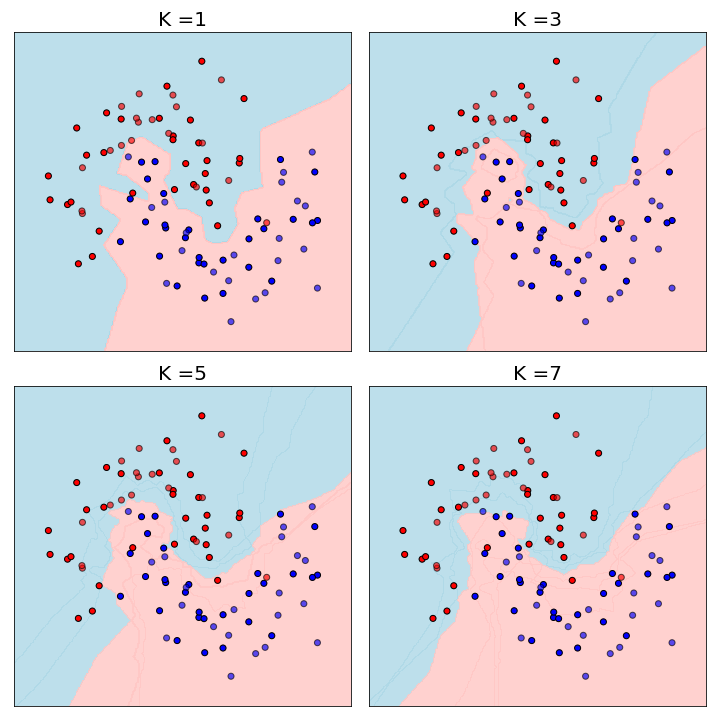
\includegraphics[width=0.7\linewidth]{../codes/statisticalAnalysisLearning/KNN/KNNMoonShape}
	\caption{Binary classification via KNN algorithm with different choices $K = 1,3, 5, 7$. Scattered points are training examples classified into two different classes (red and blue). Colored regions are corresponding decision boundaries.}
	\label{ch:statistical-learning:KNN:fig:knnmoonshape}
\end{figure}
	
	
\end{refsection}












\begin{refsection}
	\startcontents[chapters]	
	\chapter{Tree methods}\label{ch:StatisticalLearning:TreeMethods}
	\printcontents[chapters]{}{1}{}



\section{Preliminaries: entropy concepts}

For a more detailed treatment on entropy and information theory, see \autoref{ch:theory-of-probability:sec:informationTheory}.

\subsection{Concept of entropy}

\begin{definition}[entropy of a random variable]\index{entropy}\hfill
	\begin{itemize}
		\item 	Let $X$ be a discrete random variable taking values $x_k,k=1,2...$ with probability mass function 
		$$Pr(X = x_k) = p_k, k=1,2,...$$ 
		Then the entropy of $X$ is defined by
		$$H(X) = - \sum_{k\geq 1}p_k\log p_k.$$
		\item If $X$ is a continuous random variable with pdf $f(x)$, then entropy of $X$ is defined by
		$$H(X) = -\int_{-\infty}^{\infty} f(x)\log f(x) dx.$$
	\end{itemize}	
	
\end{definition}

\begin{remark}[entropy, information and probability distribution]\hfill
	\begin{itemize}
		\item Entropy is a measure of the uncertainty of a random variable: the larger the value, the uncertainty the random variable is.
		\item When the random variable is deterministic, the entropy is at the minimum.
	\end{itemize}	
\end{remark}


\begin{example}\hfill
	\begin{itemize}
		\item The entropy of the Gaussian density on $\R$ with mean $\mu$ and variance $\sigma^2$ is
		\begin{align*}
		H &= -\int_{\R} \frac{1}{\sqrt{2\pi}\sigma} \exp(-1/2((x-\mu)^2/\sigma^2))(-\log(\sqrt{2\pi}\sigma) -1/2((x-\mu)^2/\sigma^2))dx \\
		&= \frac{1}{2} + \log(\sqrt{2\pi}\sigma).
		\end{align*}
		Note that the mean $\mu$ does not enter the entropy; therefore the entropy for Gaussian distribution is translational invariant.
		\item The entropy of the exponential distribution with mean $\lambda$ and pdf
		$$f(x) = \frac{1}{\lambda}\exp(-x/\lambda)$$
		is
		$$H = -\int_0^\infty \frac{1}{\lambda} \exp(-x/\lambda)(-\log \lambda -x/\lambda) dx = \ln \lambda + 1.$$
	\end{itemize}	
\end{example}



\begin{lemma}[basic properties of entropy]\hfill
	\begin{itemize}
		\item $H(X) \geq 0$.
		\item $H(X) = 0$ if and only if there exists a $x_0$ such that $P(X=x_0) = 1$.
		\item If $X$ can take on finite number $n$ values, then $H(X) \leq \log(n)$. $H(X) = \log(n)$ if and only if $X$ is uniformly distributed. 
		\item Let $X_1,X_2,...,X_n$ be discrete valued random variables on a common probability space. Then
		$$H(X_1,X_2,...,X_n) = H(X_1) + \sum_{i=2}^n H(X_n|X_1,...,X_{n-1}).$$
		\item $H(X) + H(Y) \geq H(X,Y)$, with equality if and only if $X$ and $Y$ are independent.
	\end{itemize}
\end{lemma}
\begin{proof}
	(1) note that every term $\log(p)$ is non-positive, therefore $H(X) \geq 0$. (2) direct verification. (3)  direct verification. (4) It can be showed that $H(X,Y) = H(X|Y) + H(Y)$. (5) $H(X,Y) = H(X|Y) + H(Y) \leq H(X) + H(Y)$(using chain rule and conditioning entropy). 
\end{proof}


\begin{definition}[entropy definition in classification, empirical entropy]\index{empirical entropy}\label{ch:StatisticalLearning:TreeMethods:def:empiricalEntropy}
Let $D$ be a training data set whose examples are labeled by $K$ classes. Let $C_1,...,C_K$ be the corresponding subsets that partitions $D$ by the class labels. Then we define the \textbf{empirical entropy} of $D$ as
$$H(D) = H(D)=-\sum_{k=1}^{K} \frac{\left|C_{k}\right|}{|D|} \log \frac{\left|C_{k}\right|}{|D|}.$$	
\end{definition}


\subsection{Conditional entropy and mutual information}


\begin{definition}[conditional entropy]\index{conditional entropy}Let $X, Y$ be two discrete random variables taking values in $\cX, \cY$. 
	\begin{itemize}
		\item \textbf{Specific conditional entropy} $H(X|Y=v)$ of $X$ given $Y=y$:
		$$H(X|Y=v) = - \sum_{x \in \cX} Pr(X=x|Y=v)\log Pr(X=x|Y=y).$$
		\item \textbf{Conditional entropy} $H(X|Y)$ of $X$ given $Y$:
		$$H(X|Y) = \sum_{y\in \cY}Pr(Y = y)H(X|Y = y).$$
	\end{itemize}
Note that in general $H(X | Y) \neq H(Y | X).$
\end{definition}


\begin{definition}[mutual information, information gain]\index{mutual information}\cite{cover2012elements}
	Consider two discrete random variables $X$ and $Y$ taking values in $\cX, \cY$. The \textbf{mutual information, or information gain)} of $X$ and $Y$ is given by:
	$$I(X,Y) = H(X) - H(X|Y) = H(Y) - H(Y|X).$$
\end{definition}


\begin{lemma}[basic properties]
For two random variables $X$ and $Y$, we have
\begin{itemize}
	\item $$I(X,Y) = I(Y, X).$$
	\item $$I(X,Y) \geq 0.$$
	\item Particularly,  $I(X,Y) = 0$ if $X$ and $Y$ are independent.
\end{itemize}
\end{lemma}
	
	

\begin{proof}
	(1)(2)
	\begin{align*}
	I(X,Y)&=H(X)-H(X|Y)\\
	&=-\sum_{x\in \cX}\sum_{y\in \cY}p(x,y)\log(p(x)) + \sum_{x\in \cX}\sum_{y\in \cY} p(x|y)p(y)\log(p(x|y))\\
	& = -\sum_{x\in \cX}\sum_{y\in \cY}p(x,y)\log(p(x)) + \sum_{x\in \cX}\sum_{y\in \cY} p(x,y)\log(\frac{p(x,y)}{p(y)})\\
	& = \sum_{x\in \cX}\sum_{y\in \cY} p(x,y)\log(\frac{p(x,y)}{p(x)p(y)}) = D_{KL}(p(x,y)||p(x)p(y)) \geq 0.
	\end{align*}
	\begin{align*}
	I(X,Y)&=H(Y)-H(Y|X)\\
	&=-\sum_{x\in \cX}\sum_{y\in \cY}p(x,y)\log(p(y)) + \sum_{x\in \cX}\sum_{y\in \cY} p(y|x)p(x)\log(p(y|x))\\
	& = -\sum_{x\in \cX}\sum_{y\in \cY}p(x,y)\log(p(y)) + \sum_{x\in \cX}\sum_{y\in \cY} p(x,y)\log(\frac{p(x,y)}{p(x)})\\
	& = \sum_{x\in \cX}\sum_{y\in \cY} p(x,y)\log(\frac{p(x,y)}{p(x)p(y)}) = D_{KL}(p(x,y)||p(x)p(y)) \geq 0.
	\end{align*}
	where we use the non-negativity property of KL divergence (\autoref{ch:statistical-learning:th:KLDivergenceProperty})
	(3) When $X$ and $Y$ are independent, we have
	$$H(X|Y) = \sum_{v\in \cY}(Y=v)H(X|Y=v) = \sum_{v\in \cY}P(Y=v)H(X) = H(x).$$
\end{proof}

\begin{definition}[entropy definition in classification, empirical entropy]\index{empirical entropy}
	Let $D$ be a training data set whose examples are labeled by $K$ classes. Let $C_1,...,C_K$ be the corresponding subsets that partitions $D$ by the class labels. Then we define the \textbf{empirical entropy} of $D$ as
	$$H(D) = H(D)=-\sum_{k=1}^{K} \frac{\left|C_{k}\right|}{|D|} \log \frac{\left|C_{k}\right|}{|D|}.$$	
\end{definition}



\begin{corollary}[conditioning reduce entropy]
	Given discrete random variables $X$ and $Y$, we have
	$$H(X|Y) \leq H(X),$$ which is also known as conditioning reduces entropy (i.e., conditioning provides information); and this equality holds if and only if $X$ and $Y$ are independent.\\	
\end{corollary}


\begin{definition}[entropy definition in classification, empirical entropy]\index{empirical entropy}\label{ch:StatisticalLearning:TreeMethods:def:empiricalConditionalEntropy}\hfill
\begin{itemize}
	\item Let $D$ be a training data set whose examples are labeled by $K$ classes. Let $C_1,...,C_K$ be the corresponding subsets that partitions $D$ by the class labels.
	\item Let $A$ be one feature that takes $n$ different values $a_1,...,a_n$. We partition $D$ into $n$ subsets $D_1,...,D_n$ such that  $D_i$ is the subset of $D$ that feature $A$ is taking value $a_i$.
	\item Further denote  $D_{ik}$ as the subset of $D_i$ that belongs to class $k$.
\end{itemize}	
Then we define the \textbf{empirical conditional entropy} of $D$  conditioned on $A$ as
	$$H(D | A)=\sum_{i=1}^{n} \frac{\left|D_{i}\right|}{|D|} H\left(D_{i}\right)=-\sum_{i=1}^{n} \frac{\left|D_{i}\right|}{D |} \sum_{k=1}^{K} \frac{\left|D_{i k}\right|}{\left|D_{i}\right|} \log \frac{\left|D_{i k}\right|}{\left|D_{i}\right|}.$$	
\end{definition}

\section{Decision tree learning}


\subsection{Basic concepts}
\begin{mdframed}
\textbf{General remarks}:
\begin{itemize}
	\item Decision tree essentially performs a greedy search in the hypothesis space, based on some metric on each greedy step(e.g., maximum mutual information gain), to find a hypothesis, i.e., a decision tree that sort the data.
	\item If there is no contradictory examples(i.e. two examples with the same $x$ yet produce different $y$), there will exist a decision tree perfectly predict $y$ based on $x$.
\end{itemize}
\end{mdframed}






\begin{figure}[H]
	\centering
	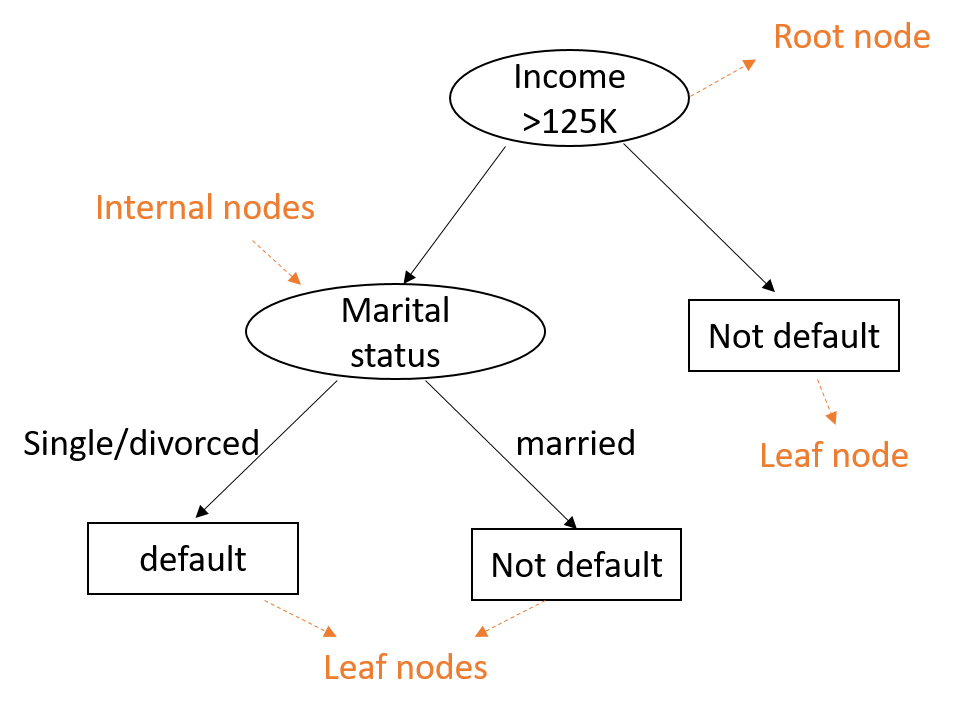
\includegraphics[width=0.7\linewidth]{../figures/statisticalLearning/treeMethods/decisionTreeClassifierScheme}
	\caption{}
	\label{fig:decisiontreeclassifierscheme}
\end{figure}






\subsection{The generic algorithm}


\begin{algorithm}[H]
	\SetAlgoLined
	\KwIn{training data set $D = \{(x_1,y_1), (x_2,y_2),...,(x_N,y_N)\}$, threshold $\epsilon$, feature set $\cA$. We assume $y$ has being $K$ classes and therefore the samples can be divided into $C_1,...,C_k$.}
	
	
	If all samples in $D$ belongs to the same class $C_i$, label current node as $C_i$. Stop splitting.
	
	If $A = \emptyset$, label label current node as the dominant class in $D$. Stop splitting.
	
	\ForEach{feature $A \in \cA$}{
		Compute empirical entropy for $D$ (\autoref{ch:StatisticalLearning:TreeMethods:def:empiricalEntropy}) via
		$$H(D)=-\sum_{k=1}^{K} \frac{\left|C_{k}\right|}{|D|} \log \frac{\left|C_{k}\right|}{|D|}$$
		where $C_k$ is the count of samples labeled as class $k$.
		
		Compute emprical condtional entropy for $D$ conditioned on $A$ (\autoref{ch:StatisticalLearning:TreeMethods:def:empiricalConditionalEntropy}):
		$$H(D | A) = -\sum_{i=1}^{n} \frac{\left|D_{i}\right|}{D |} \sum_{k=1}^{K} \frac{\left|D_{i k}\right|}{\left|D_{i}\right|} \log _{2} \frac{\left|D_{i k}\right|}{\left|D_{i}\right|},$$
		
		
		
		Compute information gain
		$$IG(D, A) = H(D) - H(D|A)$$
	}
	
	Select the feature $A$ with the maximum information gain.
	
	\uIf{$IG(D, A) < \epsilon$
	}{
		If , stop splitting. Label current node with the dominant class in $D$. 
	}\uElse{
		Partition $D$ into $D_1,...,D_n$ based on each possible value $a_i$ of feature $A$. Lebel current node with the dominant class in $D$. \\
		For each non-empty set $D_i$, create a child node.For each $i$ child node Using $D_i$ as the training data and $\cA - A$ as the feature set
		
	}
	
	\KwOut{the tree model}
	\caption{ID3 classification decision tree algorithm}
\end{algorithm}




\section{Classification tree}

\subsection{Basics}


\begin{method}[Hunt's generic algorithm for decision tree construction]\cite[152]{tan2013introduction}
Hunt's algorithm is a recursive algorithm that grows a decision tree in a recursive fashion by partitioning the training examples into successively purer subsets. Let $\cD_t$ be the set of training examples that are associated with node $t$ and $y = {y1, y2, . . . , yc}$ be
the class labels. The following is a recursive definition of Hunt's algorithm.
\begin{itemize}
	\item If all the records in Dt belong to the same class yt, then t is a leaf node labeled as yt.
	\item If Dt contains records that belong to more than one class, an attribute test condition is selected to partition the records into smaller subsets. A child node is created for each outcome of the test condition and the records in Dt are distributed to the children based on the outcomes. The algorithm is then recursively applied to each child node
\end{itemize}	
\end{method}

\begin{definition}[impurity measures]
Common impurity measures for examples in node are given by
\begin{itemize}
	\item $$Entropy = -\sum_{i=1}^K p_i\ln p_i.$$
	\item $$Gini = -\sum_{i=1}^K p_i\ln p_i.$$
	\item $$Classifying~error = 1 - \max (p_1, p_2,...,p_K).$$
\end{itemize}	
where $p_i$ is the fraction examples with class label $i$ (there are totally $K$ classes).
\end{definition}


\begin{example}
Consider the following computation examples:
\begin{itemize}
	\item A node contains 4 examples with label 1 and 6 examples with label 0. Then
	\begin{align*}
	Gini &= 1 - 0.4^2 - 0.6^2 = 0.48 \\
	Entropy &= -0.4\ln(0.4) - 0.6\ln(0.6) = 0.673 \\
	Error &= 1 - \max(0.4,0.6) = 0.4 
	\end{align*}
	\item A node contains 9 examples with label 1 and 1 example with label 0. Then
	\begin{align*}
	Gini &= 1 - 0.1^2 - 0.9^2 = 0.18 \\
	Entropy &= -0.1\ln(0.1) - 0.9\ln(0.9) = 0.326 \\
	Error &= 1 - \max(0.1,0.9) = 0.1 
	\end{align*}
\end{itemize}
\end{example}


\begin{figure}[H]
	\centering
	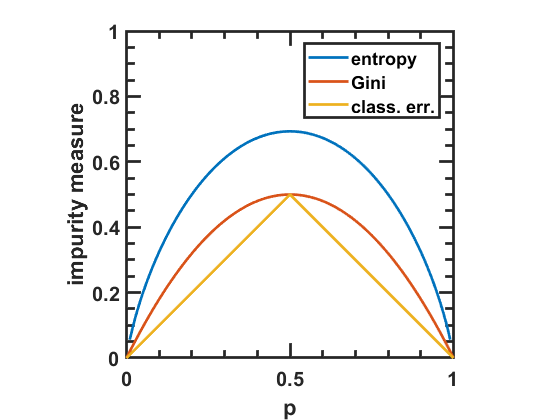
\includegraphics[width=0.5\linewidth]{../figures/statisticalLearning/treeMethods/impurityMeasure}
	\caption{Different types of impurity measure. Entropy function, Gini function and classification error function.}
	\label{ch:statistical-learning:fig:impuritymeasure}
\end{figure}



\begin{figure}[H]
	\centering	
	\begin{subfigure}[b]{0.42\textwidth}
		\centering
		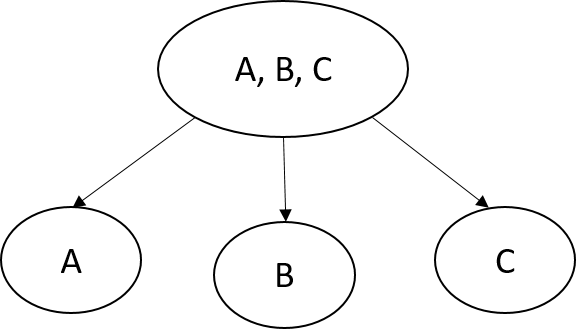
\includegraphics[width=0.7\linewidth]{../figures/statisticalLearning/treeMethods/decisionTreeMultiwaySplit}
		\caption{Multi-way split in a node on one attribute with three types values.}
	\end{subfigure}\\
	\begin{subfigure}[b]{1.0\textwidth}
		\centering
		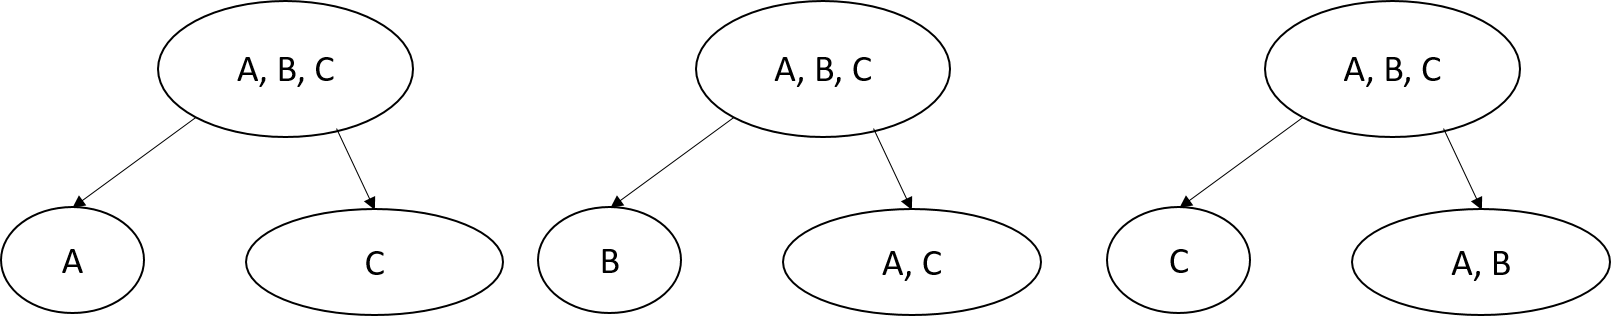
\includegraphics[width=0.7\linewidth]{../figures/statisticalLearning/treeMethods/decisionTreeBinarySplit}
		\caption{A recursive tree representation of the partition.}
	\end{subfigure}
	\caption{Demonstration of a tree and input space partition.}
\end{figure}


\begin{method}[decision tree classifier splitting methods]
Consider a set of items of $K$ classes. Let $p_i$ be the fraction of items labeled with class $i$. 


\begin{itemize}
	\item Gini impurity: 
	$$Gini(p_1,...,p_K) = 1 - \sum_{i=1}^K p_i^2.$$
	\item Information gain
	$$IG = H(T) - H(p|a) = -\sum_{i=1}^K p_i\log(p_i) - \sum_a p(a)\sum_{i=1}^K(-Pr(i|a))$$
	\item Information gain ratio
	
	$$IGR = \frac{IG}{H(T)}.$$
\end{itemize}	
\end{method}

\begin{remark}[interpret Gini impurity]
Gini impurity is a measure of how often a randomly chosen element from the set would be incorrectly labeled if it was randomly labeled according to the distribution of labels in the subset.	
\begin{align*}
I_G &= \sum_{i=1}^K p_i \sum_{j\neq i}p_k\\
&=\sum_{i=1}^K p_i(1-p_i) \\
&=\sum_{i=1}^K p_i-p_i^2 \\
&=1 - \sum_{i=1}^K p_i^2
\end{align*}	
\end{remark}

\begin{remark}[the need for information gain ratio]
Information gain ratio biases the decision tree against considering attributes with a large number of distinct values. So it solves the drawback of information gain—namely, information gain applied to attributes that can take on a large number of distinct values might learn the training set too well. For example, suppose that we are building a decision tree for some data describing a business's customers. Information gain is often used to decide which of the attributes are the most relevant, so they can be tested near the root of the tree. One of the input attributes might be the customer's credit card number. This attribute has a high information gain, because it uniquely identifies each customer, but we do not want to include it in the decision tree: deciding how to treat a customer based on their credit card number is unlikely to generalize to customers we haven't seen before.	
\end{remark}




\begin{remark}[the Iris dataset]\index{Iris dataset}
The Iris dataset contains attributes, Petal Length, Petal Width, Sepal Length and Sepal width and three classes, setosa, versicolor and virginica.	

\end{remark}




\begin{remark}[perfect classification tree]
If the input variables in a classification problems are all categorical, then there exist a classificiation tree perfectly classify all the training examples.	
\end{remark}



\begin{remark}[classification tree stop growing criterion]
A classification tree can grow until all the leave node are pure. Additional parameters controlling the stopping criterion are
\begin{itemize}
	\item maximum depth: the maximum depth of the tree.
	\item minimum sample size for splitting: the minimum sample number in a node for splitting.
	\item information gain threshold: the minimum information gain when splitting a node. 
	\item Gini impurity decreasing threshold: the minimum Gini impurity decreasing when splitting a node.
\end{itemize}	
\end{remark}




\subsection{ID3 and ID4.5 algorithm}

\begin{algorithm}[H]
	\SetAlgoLined
	\KwIn{training data set $D = \{(x_1,y_1), (x_2,y_2),...,(x_N,y_N)\}$, threshold $\epsilon$, feature set $\cA$. We assume $y$ has being $K$ classes and therefore the samples can be divided into $C_1,...,C_k$.}
	
	
	If all samples in $D$ belongs to the same class $C_i$, label current node as $C_i$. Stop splitting.
	
	If $A = \emptyset$, label label current node as the dominant class in $D$. Stop splitting.
	
	\ForEach{feature $A \in \cA$}{
		Compute empirical entropy for $D$ (\autoref{ch:StatisticalLearning:TreeMethods:def:empiricalEntropy}) via
		$$H(D)=-\sum_{k=1}^{K} \frac{\left|C_{k}\right|}{|D|} \log \frac{\left|C_{k}\right|}{|D|}$$
		where $C_k$ is the count of samples labeled as class $k$.
		
		Compute emprical condtional entropy for $D$ conditioned on $A$ (\autoref{ch:StatisticalLearning:TreeMethods:def:empiricalConditionalEntropy}):
		$$H(D | A) = -\sum_{i=1}^{n} \frac{\left|D_{i}\right|}{D |} \sum_{k=1}^{K} \frac{\left|D_{i k}\right|}{\left|D_{i}\right|} \log _{2} \frac{\left|D_{i k}\right|}{\left|D_{i}\right|},$$
		
		
		
		Compute information gain
		$$IG(D, A) = H(D) - H(D|A)$$
	}
	
	Select the feature $A$ with the maximum information gain.
	
	\uIf{$IG(D, A) < \epsilon$
	}{
		If , stop splitting. Label current node with the dominant class in $D$. 
	}\uElse{
		Partition $D$ into $D_1,...,D_n$ based on each possible value $a_i$ of feature $A$. Lebel current node with the dominant class in $D$. \\
		For each non-empty set $D_i$, create a child node.For each $i$ child node Using $D_i$ as the training data and $\cA - A$ as the feature set
		
	}
	
	\KwOut{the tree model}
	\caption{ID3 classification decision tree algorithm}
\end{algorithm}


\begin{remark}
	Because ID3 algorithm only have tree growth but not tree pruning, ID3 algorithm can easily lead to overfitting.
\end{remark}

\subsection{Tree pruning}

\begin{remark}[motivation for tree pruning]\hfill
	\begin{itemize}
		\item Decision tree algorithms usually generate a tree that is too large and overfits the training data.
		\item However, it is hard to decide when the tree growing steps should stop because the addition of an extra node might give dramatic error reduction.
	\end{itemize}	
	
\end{remark}

\href{http://faculty.cs.tamu.edu/ioerger/cs633-spr10/pruning.ppt}{link}

\begin{method}[reduced-error pruning for classification/regression tree]
	\begin{itemize}
		\item Classify examples in the validation set.
		\item From root to leaf for each node
		\begin{itemize}
			\item Sum the errors over entire subtree
			\item Calculate the error if the subtree is converted to a leaf node with major class label (or the mean of the subtree in a regression tree).
			\item Record the error reduction.
			\item Replace subtree with leaf node with highest reduction in error.
			\item Repeat until error no longer reduced.
		\end{itemize}
	\end{itemize}	
\end{method}



\subsection{CART algorithm}

\begin{algorithm}[H]
	\SetAlgoLined
	\KwIn{training data set $D = \{(x_1,y_1), (x_2,y_2),...,(x_N,y_N)\}$, threshold $\epsilon$, feature set $\cA$. We assume $y$ has being $K$ classes and therefore the samples can be divided into $C_1,...,C_k$.}
	
	
	If all samples in $D$ belongs to the same class $C_i$, label current node as $C_i$. Stop splitting.
	
	If $A = \emptyset$, label label current node as the dominant class in $D$. Stop splitting.
	
	\ForEach{feature $A \in \cA$}{
		Compute empirical entropy for $D$ (\autoref{ch:StatisticalLearning:TreeMethods:def:empiricalEntropy}) via
		$$H(D)=-\sum_{k=1}^{K} \frac{\left|C_{k}\right|}{|D|} \log \frac{\left|C_{k}\right|}{|D|}$$
		where $C_k$ is the count of samples labeled as class $k$.
		
		Compute emprical condtional entropy for $D$ conditioned on $A$ (\autoref{ch:StatisticalLearning:TreeMethods:def:empiricalConditionalEntropy}):
		$$H(D | A) = -\sum_{i=1}^{n} \frac{\left|D_{i}\right|}{D |} \sum_{k=1}^{K} \frac{\left|D_{i k}\right|}{\left|D_{i}\right|} \log _{2} \frac{\left|D_{i k}\right|}{\left|D_{i}\right|},$$
		
		
		
		Compute information gain
		$$IG(D, A) = H(D) - H(D|A)$$
	}
	
	Select the feature $A$ with the maximum information gain.
	
	\uIf{$IG(D, A) < \epsilon$
	}{
		If , stop splitting. Label current node with the dominant class in $D$. 
	}\uElse{
		Partition $D$ into $D_1,...,D_n$ based on each possible value $a_i$ of feature $A$. Lebel current node with the dominant class in $D$. \\
		For each non-empty set $D_i$, create a child node.For each $i$ child node Using $D_i$ as the training data and $\cA - A$ as the feature set
		
	}
	
	\KwOut{the tree model}
	\caption{ID3 classification decision tree algorithm}
\end{algorithm}



\subsection{Examples}


\begin{figure}[H]
	\centering
	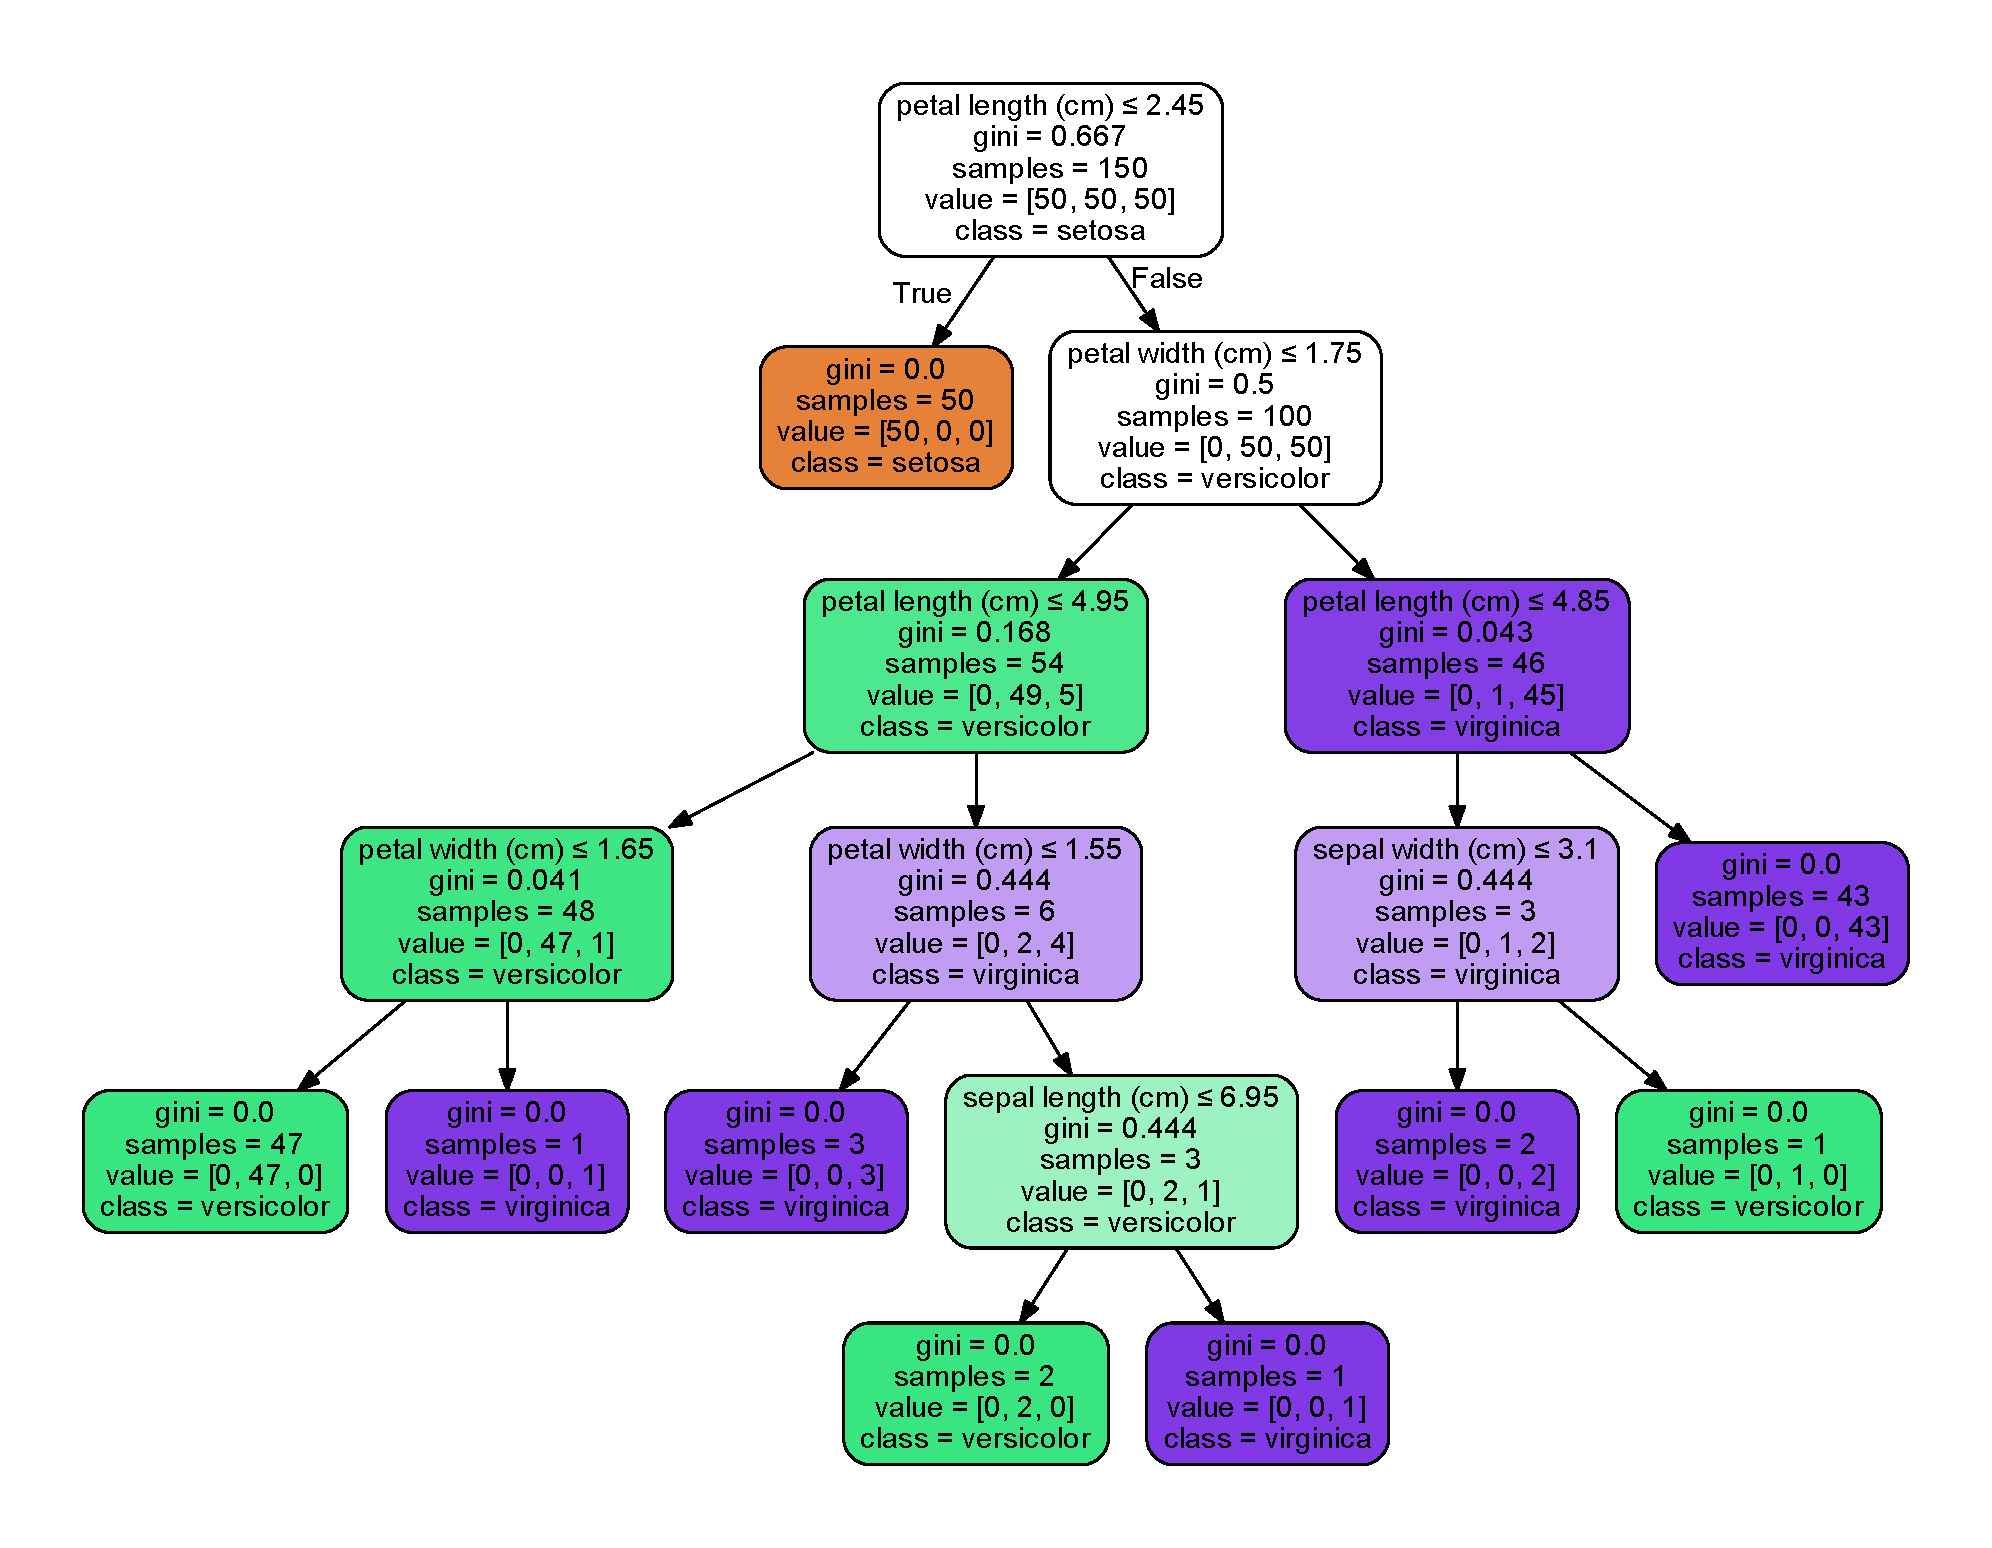
\includegraphics[width=0.8\linewidth]{../figures/statisticalLearning/treeMethods/IrisDecisionTree_Gini}
	\caption{The visualization of the decision tree classifier for Iris data set. The tree grows until all examples are classified correctly. The splitting criterion is Gini impurity. }
	\label{fig:irisdecisiontreegini}
\end{figure}

\begin{figure}[H]
	\centering
	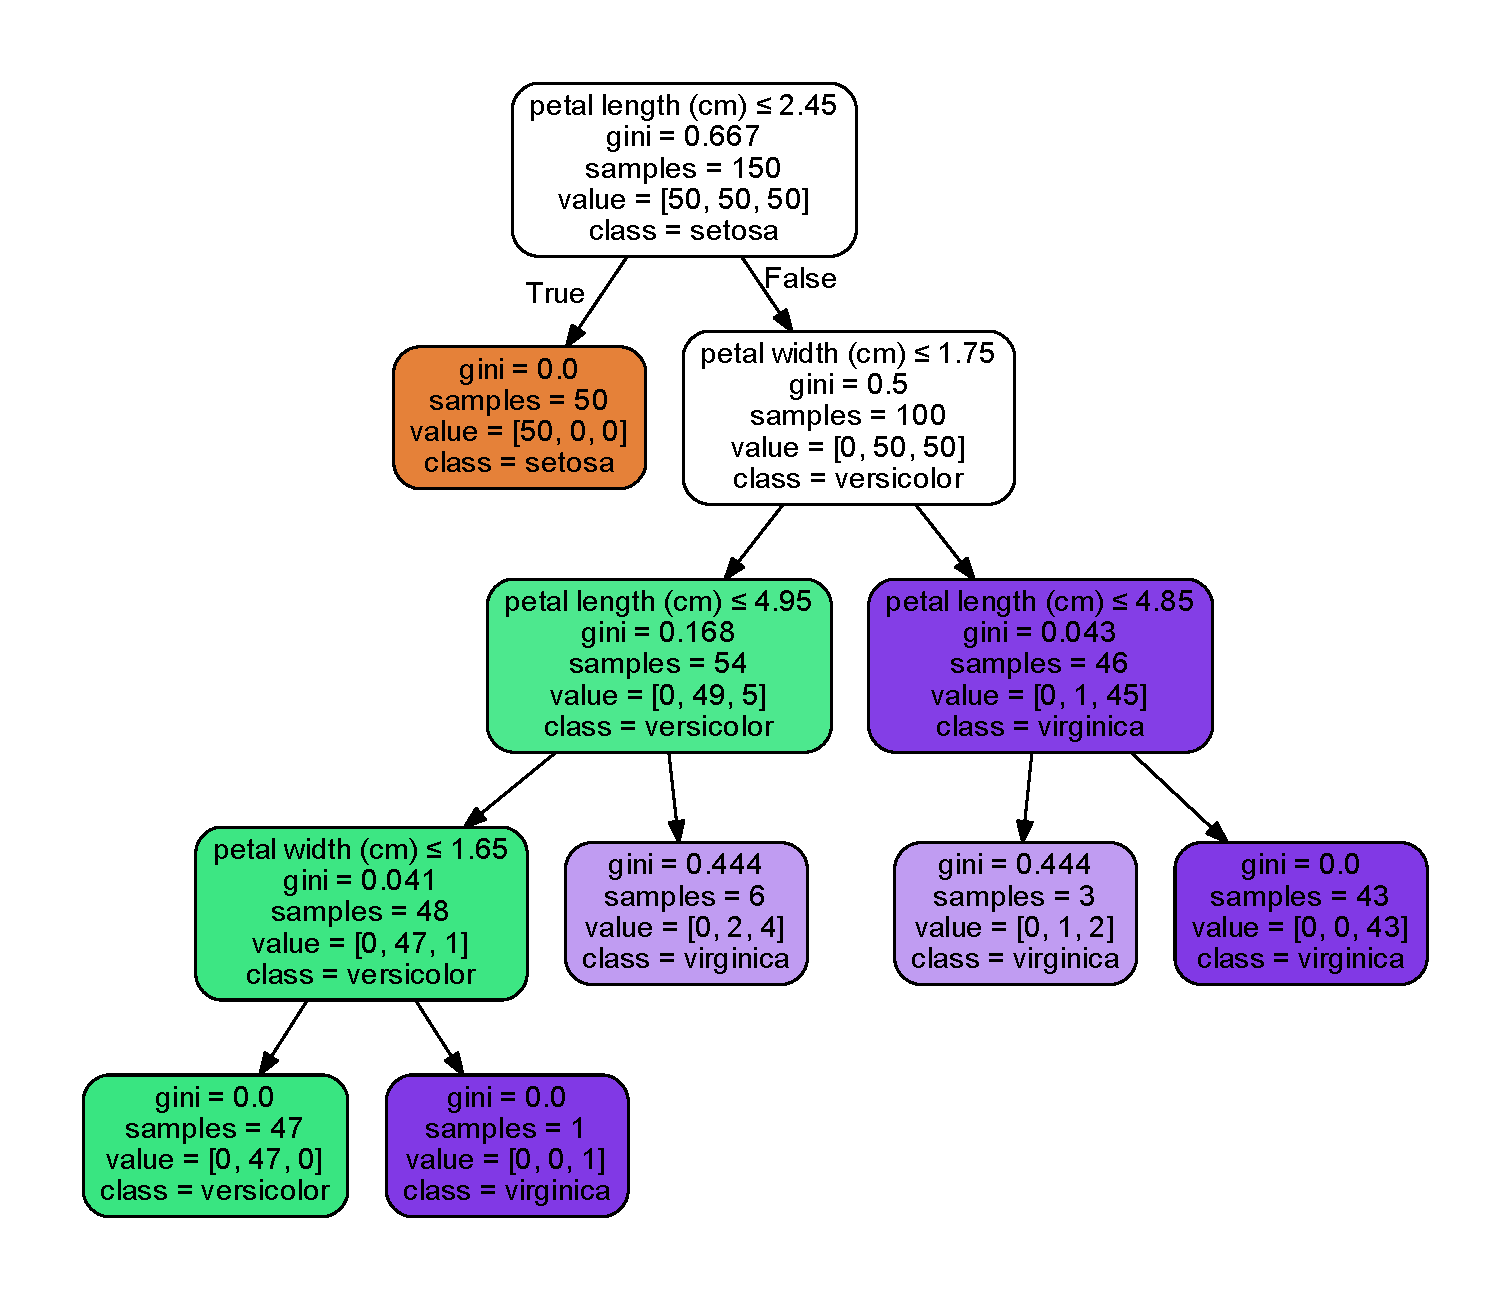
\includegraphics[width=0.7\linewidth]{../figures/statisticalLearning/treeMethods/IrisDecisionTree_minSamplesGini}
	\caption{The visualization of the decision tree classifier for Iris data set. The tree grows until examples in each node is smaller than 10. The splitting criterion is Gini impurity.}
	\label{fig:irisdecisiontreeminsamplesgini}
\end{figure}

\begin{figure}[H]
	\centering
	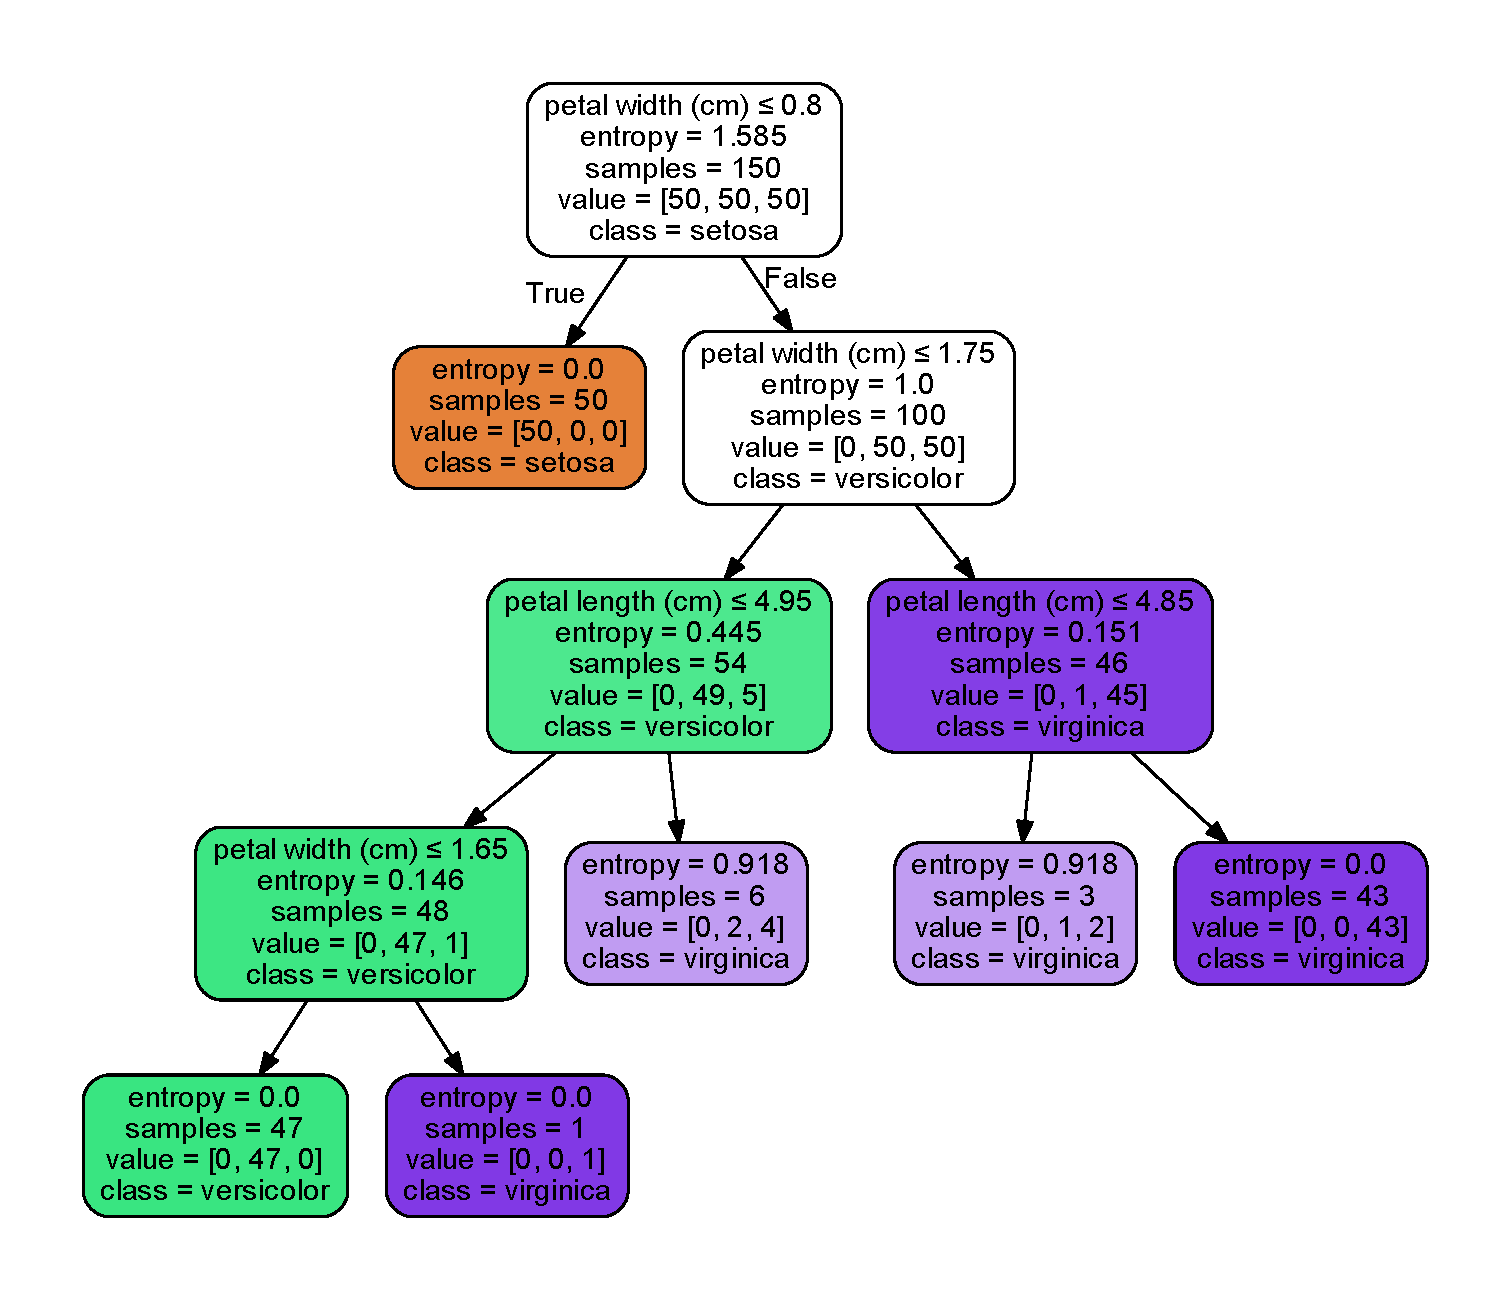
\includegraphics[width=0.7\linewidth]{../figures/statisticalLearning/treeMethods/IrisDecisionTree_minSamplesEntropy}
	\caption{The visualization of the decision tree classifier for Iris data set. The tree grows until examples in each node is smaller than 10. The splitting criterion is entropy and information gain.}
	\label{fig:irisdecisiontreeminsamplesentropy}
\end{figure}



\section{Regression tree}

\begin{definition}[tree splitting]
Consider the predicators $X_1,...,X_p$, we want to select the $j$ predicator and a value $s$, such that for the pair of half-planes:
$$R_1(j,s) = \{X|X_j < s\}, R_2(j,s) = \{X|X_j \geq s\},$$
the equation
$$\sum_{i:x_i\in R_1(j,s)} (y_i - \hat{y}_{R_1})^2 + \sum_{i:x_i\in R_2(j,s)} (y_i - \hat{y}_{R_2})^2$$
is minimized. In here, $\hat{y}_{R_1}$ is the mean response for the training observations in $R_1$ and $\hat{y}_{R_2}$ is the mean response for the training observations in $R_2$.
\end{definition}


\begin{remark}[another equivalent formulation on variance reduction]
The variance reduction of a node is defined as the total reduction of the variance of the target variable $y$ due to the split at this node. The change of variance is given by
\begin{align*}
\Delta V = \frac{1}{\abs{S_N}^2} \sum_{i \in S_N}\sum{j\in S_N}\frac{1}{2}(x_i-x_j)^2
\end{align*}	
	
\end{remark}


\begin{remark}[technical procedures of tree splitting]
Loop through every predicator $X_i$, to choose optimal $s$ based on two situations:
\begin{itemize}
	\item If $X_i$ is discrete variable(such as, 0 and 1), then we simply loop through the discrete values to select the best one.
	\item If $X_i$ is a continuous variable, then we can first sort the training examples based on $X_i$, and test all possible splits using all values for variable $X_i$ to select the optimal value.\footnote{Depending on the number of examples, more efficient splitting based on sorting, binary search, etc. will be considered.}
\end{itemize}	
\end{remark}



The regression tree assume a model of the form
$$f(X) = \sum_{m=1}^M c_m 1(X\in R_m)$$
where $R_1,...,R_m$ represent a partition of the feature space $\cX$.



\begin{figure}[H]
\centering	
\begin{subfigure}[b]{0.42\textwidth}
	\centering
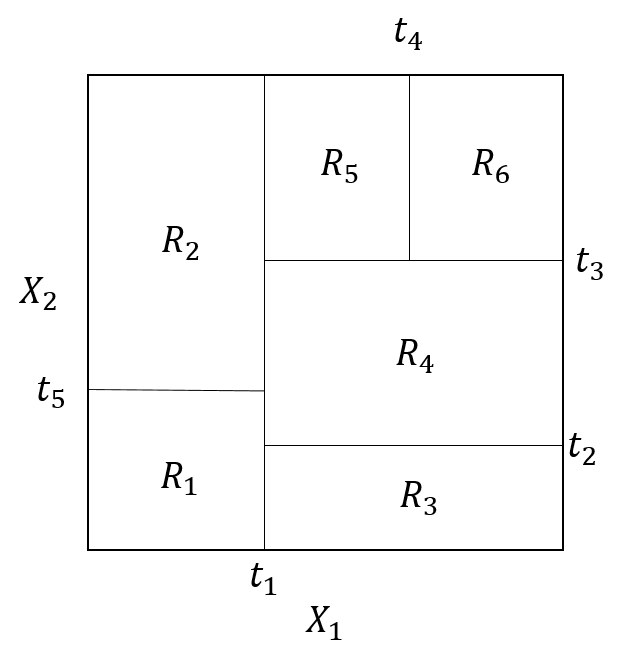
\includegraphics[width=0.7\linewidth]{../figures/statisticalLearning/treeMethods/2DInputSpacePartitionDemo}
\caption{Demonstration of a partition of a 2D input space.}
\end{subfigure}\quad
\begin{subfigure}[b]{0.42\textwidth}
	\centering
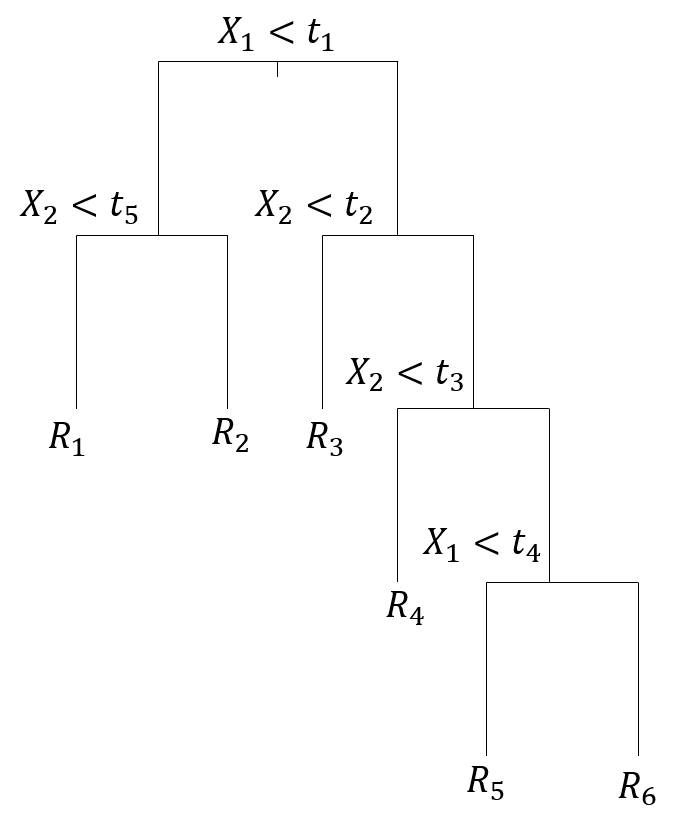
\includegraphics[width=0.7\linewidth]{../figures/statisticalLearning/treeMethods/2DInputSpacePartitionRecursiveTreeDemo}
\caption{A recursive tree representation of the partition.}
\label{fig:2DInputSpacePartitionRecursiveTreeDemo}
\end{subfigure}
\caption{Demonstration of a tree and input space partition.}
\end{figure}



\begin{remark}[splits, depths, and the number of output levels]\hfill
\begin{itemize}
	\item Let the number of splits be $S$, then the number of output levels $M$ is given by
	$$M = S + 1.$$
	\item Let the number of depth be $M$, then the number of output levels $M$ is bounded by
	$$D+ 1 \leq  M \leq 2^D.$$
\end{itemize}	
\end{remark}


\begin{figure}[H]
	\centering	
	\begin{subfigure}[b]{0.45\textwidth}
		\centering
		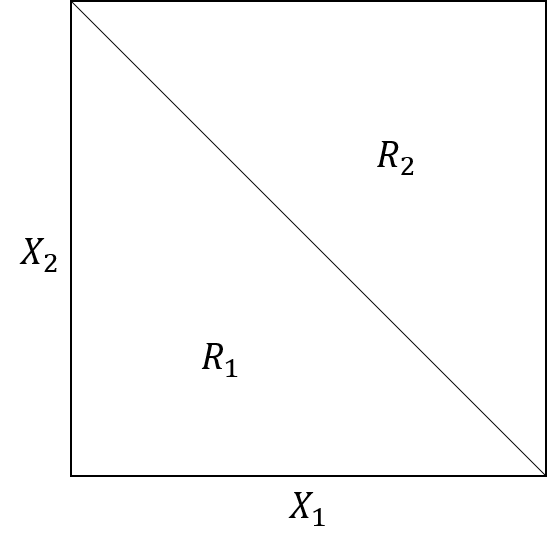
\includegraphics[width=0.7\linewidth]{../figures/statisticalLearning/treeMethods/2DInputSpacePartitionFailureExampleOne}
		\caption{A partition of 2D input space that cannot be represented by a recursive tree. However, it can be represented after a linear transformation to the input space.}
	\end{subfigure}\quad
	\begin{subfigure}[b]{0.45\textwidth}
		\centering
		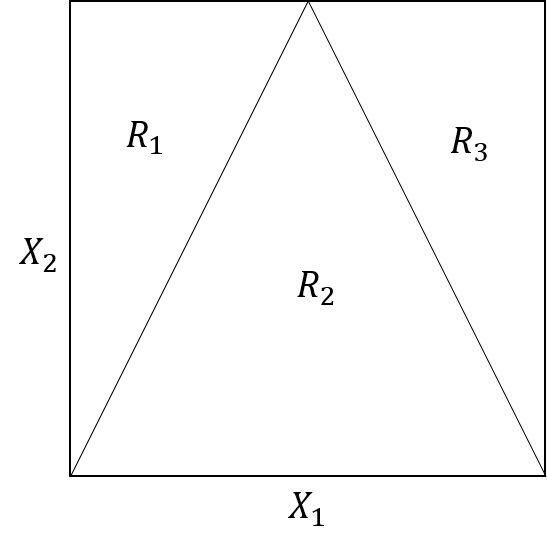
\includegraphics[width=0.7\linewidth]{../figures/statisticalLearning/treeMethods/2DInputSpacePartitionFailureExampleTwo}
		\caption{A partition of 2D input space that cannot be represented by a recursive tree. No linear transformation can make it representable.}
		\label{fig:2DInputSpacePartitionRecursiveTreeFailure}
	\end{subfigure}
	\caption{2D input space partitions cannot be represented by a recursive tree.}
\end{figure}


\begin{figure}[H]
	\centering
\begin{subfigure}[t]{0.45\textwidth}
	\centering
	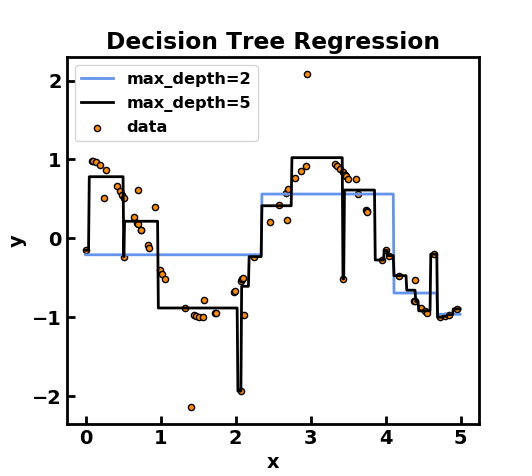
\includegraphics[width=1\linewidth]{../figures/statisticalLearning/treeMethods/decisionTreeRegressionExample}
	\caption{Decision tree regression for training examples generated by $y = \cos(2x)$ plus large deviation at some points. Decision trees used have maximum depth of 2 and 5. Code: decisionTreeRegressionExample.py}
\end{subfigure}\quad
	\begin{subfigure}[t]{0.45\textwidth}
	\centering
	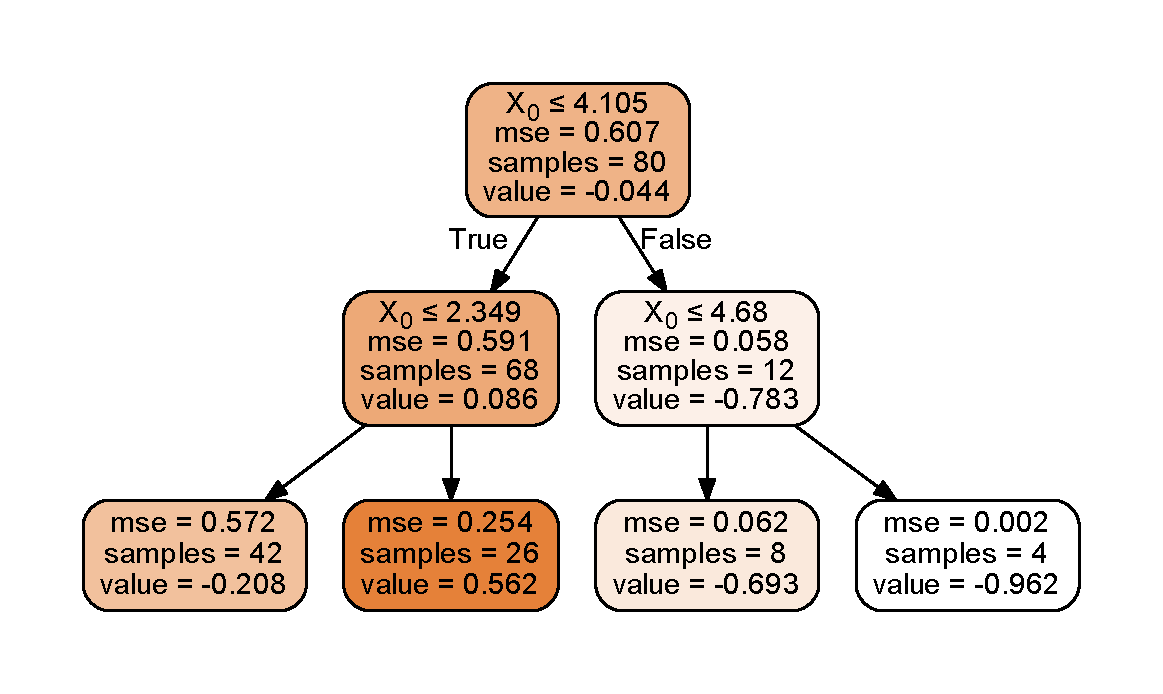
\includegraphics[width=1\linewidth]{../figures/statisticalLearning/treeMethods/RegressionTree_maxdepth2}
	\caption{Rendering of the regression tree with maximum depth of 2.}
\end{subfigure}
\caption{Regression tree demonstration.}
	\label{fig:decisiontreeregressionexample}
\end{figure}


\subsection{CART algorithm}

\begin{algorithm}[H]
	\SetAlgoLined
	\KwIn{training data set $D = \{(x_1,y_1), (x_2,y_2),...,(x_N,y_N)\}$, threshold $\epsilon$, feature set $\cA$. We assume $y$ has being $K$ classes and therefore the samples can be divided into $C_1,...,C_k$.}
	
	
	If all samples in $D$ belongs to the same class $C_i$, label current node as $C_i$. Stop splitting.
	
	If $A = \emptyset$, label label current node as the dominant class in $D$. Stop splitting.
	
	\ForEach{feature $A \in \cA$}{
		Compute empirical entropy for $D$ (\autoref{ch:StatisticalLearning:TreeMethods:def:empiricalEntropy}) via
		$$H(D)=-\sum_{k=1}^{K} \frac{\left|C_{k}\right|}{|D|} \log \frac{\left|C_{k}\right|}{|D|}$$
		where $C_k$ is the count of samples labeled as class $k$.
		
		Compute emprical condtional entropy for $D$ conditioned on $A$ (\autoref{ch:StatisticalLearning:TreeMethods:def:empiricalConditionalEntropy}):
		$$H(D | A) = -\sum_{i=1}^{n} \frac{\left|D_{i}\right|}{D |} \sum_{k=1}^{K} \frac{\left|D_{i k}\right|}{\left|D_{i}\right|} \log _{2} \frac{\left|D_{i k}\right|}{\left|D_{i}\right|},$$
		
		
		
		Compute information gain
		$$IG(D, A) = H(D) - H(D|A)$$
	}
	
	Select the feature $A$ with the maximum information gain.
	
	\uIf{$IG(D, A) < \epsilon$
	}{
		If , stop splitting. Label current node with the dominant class in $D$. 
	}\uElse{
		Partition $D$ into $D_1,...,D_n$ based on each possible value $a_i$ of feature $A$. Lebel current node with the dominant class in $D$. \\
		For each non-empty set $D_i$, create a child node.For each $i$ child node Using $D_i$ as the training data and $\cA - A$ as the feature set
		
	}
	
	\KwOut{the tree model}
	\caption{ID3 classification decision tree algorithm}
\end{algorithm}



\subsection{Examples}


\begin{example}
	Consider the following training samples \\
	\begin{tabular}{|c|c|c|c|c|c|c|c|c|c|c|}
		\hline 
		$x_i$ & 1 & 2 & 3 & 4 & 5 & 6 & 7 & 8 & 9 & 10 \\ 
		\hline 
		$y_i$ & 5.56 & 5.70 & 5.91 & 6.40 & 6.80 & 7.05 & 8.90 & 8.70 & 9.00 & 9.05 \\ 
		\hline 
	\end{tabular} 	
	
	
	To get the split point $s$ such that we have partitions on $\R$ given by
	$$R_1\in \{x|x\geq s\}, R_2=\{x > s\}.$$
	
	We then iterate over split point candidates of $\{1.5, 2.5, 3.5, ..., 9.5 \}$, such that
	$$m(s) = \sum_{x_i\in R_1}(y_i - c_1)^2 + \sum_{x_i\in R_2}(y_i - c_2)^2,$$
	where $$c_1 = \frac{1}{N_1}\sum_{x_i\in R_1}y_i, c_2 = \frac{1}{N_2}\sum_{x_i\in R_2}y_i. $$
	
	Then we can find when $s = 6.5$, $m(s)$ has a minimum value; that is $s=6.5$ is selected as the first split point.
\end{example}



\section{Note on bibliography}

\end{refsection}

\begin{refsection}
	\startcontents[chapters]	


\chapter{Ensemble and boosting methods}
	\printcontents[chapters]{}{1}{}

\section{Overview}



Building an ensemble usually consists of two steps:
\begin{itemize}
	\item Construct base learners using varying models, samples, model parameters, partitions of the input space.
	\item Combining base learners together by voting.
\end{itemize}


\begin{remark}[model averaging method]\cite[5]{seni2010ensemble}
	
\end{remark}
\begin{itemize}
	\item Bayesian model avearging sums estimates of possible models, weighted by their posterior probabilities.
	\item Bagging bootstraps the training data set and build different model. Then majority vote is taken.
	\item Random forest consists of models built from subsets randomly sampled from data sets. 
	\item AdaBoost iteratively build models by varying case weights (up-weighting cases with large current errors and down-weighting those accurately estimated) 
\end{itemize}


\subsection{Benefits of major vote}

\begin{figure}
\centering
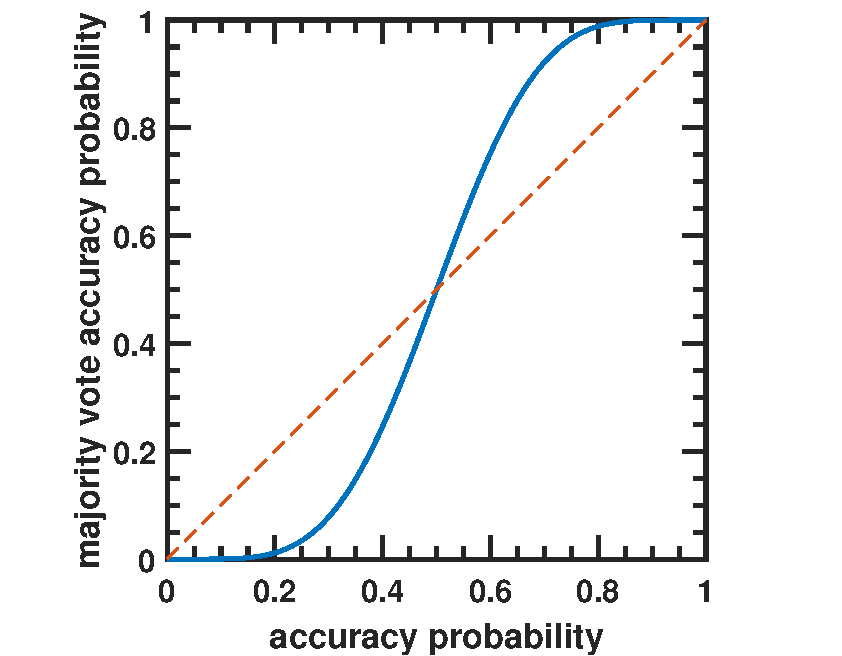
\includegraphics[width=0.6\linewidth]{../figures/statisticalLearning/ensembleMethods/majorVoteAccuracyProbabilityVsSingleVote}
\caption{Code: majorVoteProbabilityCompare.m. }
\label{fig:majorVoteAccuracyProbabilityVsSingleVote}
\end{figure}

\section{Bagging}

\begin{algorithm}[H]
	\SetAlgoLined
	\KwIn{Training data $(x_1,y_1),...,(x_m,y_m)$ where $x_i\in X$, $y_i\in Y = \cY$; Base learning alogorithm $\cL$; Number of base learners $T$.}
	Initialize $t = 1$.
	\Repeat{ $t = T$ }{
		Generate bootstrapped sample $D_t$ from $D$ via sampling with replacement.\\
		Train weak learner using bootstrapped sample $D_t$. \\
		Set $t = t + 1.$
	}
	Construct the final classifier/regressors $H$: 
	The averaging method for regression
	$$H(x) = \frac{1}{K}\sum_{i=1}^K h_i(x).$$
	and the voting method for classification
	$$H(x) = \arg\max_{y\in \cY} \sum_{i=1}^K \bm{1}(h_i(x) = y).$$
	\KwOut{$H(x)$}
	\caption{Bagging algorithm}\index{Bagging}
\end{algorithm}



\section{Adaboost}

\subsection{Basics}

\subsection{Adaboost classifier}
\begin{algorithm}[H]
	\SetAlgoLined
	\KwIn{Training data $(x_1,y_1),...,(x_m,y_m)$ where $x_i\in X$, $y_i\in Y = \{-1,1\}$}
	Initialize sample $w_1(i) = 1/m$ and set $t = 1$. \\
	\Repeat{ $t = T$ }{
		Train weak learner using distributin $D_t$.\\
		Get weak classifier $h_t: X\to \R.$\\
		Choose $\alpha_t \in \R, \alpha_t > 0$.\\
		Update sample weights:
		$$w_{t+1}(i) = \frac{w_t(i)\exp(-\alpha_t y_i h_t(x_i))}{Z_t}$$
		where
		$$Z_t = \sum_{i=1}^N w_t(i)\exp(-\alpha_t y_i h_t(x_i))$$
		is the normalization factor.\\
		$t = t+1.$
	}
	Construct the final classifier:
	$$H(x) = sign(\sum_{t=1}^T \alpha_t h_t(x)).$$	\\
	\KwOut{$H(x)$}
	\caption{Adaboost algorithm}\index{Adaboost}
\end{algorithm}


\begin{remark}[weight increasing for misclassified examples]
	If an classifier is doing wrong at example $i$, then $y_i h_t(x_i) < 0$, and the weight of example $i$ will be up-weighted.
\end{remark}



\begin{lemma}
$$\frac{1}{m}\sum_{i=1}^m \delta(H(x_i)\neq y_i) \leq \frac{1}{m}\exp(-y_i f(x_i)) = \prod_t Z_t$$
where $f(x) = \sum_t \alpha_t h_t(x), H(x) = sign(f(x)).$

Let $\epsilon_t$ be the weighted training error given as
$$\epsilon_t = \sum_{i=1}^m D_t(i) \delta(h_t(x_i) \neq y_i).$$
If $\epsilon_t < 0.5$, then
$$\frac{1}{m}\sum_{i=1}^m \delta(H(x_i)\neq y_i) \leq  \prod_{t=1}^T Z_t \leq \exp(-2\sum_{t=1}^T(1/2 - \epsilon_t)^2)$$
\end{lemma}


\begin{remark}[interpretation]
The training error upper bound will decrease exponentially fast.
\end{remark}


\begin{figure}[H]
	\centering
	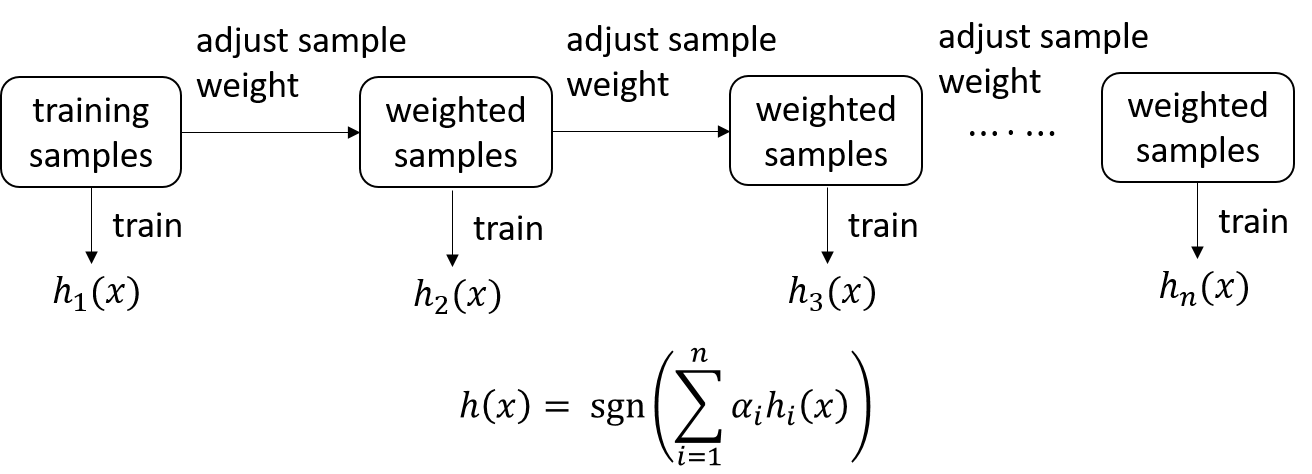
\includegraphics[width=0.7\linewidth]{../figures/statisticalLearning/ensembleMethods/boostingLearningScheme}
	\caption{}
	\label{fig:boostinglearningscheme}
\end{figure}


\subsection{Adaboost regressor}



\subsection{Additive model framework}

\subsubsection{The framework}

Consider a forward stagewise additive model with
\begin{itemize}
	\item loss function set to 
	$$L(y,h(x)) = \exp(-yh(x))$$
	\item the total loss is
	$$\sum_{i=1}^N L(y_i, \sum_{m=1}^M \beta_Mh_m(x_i)),$$
	\item optimal solution at step $m$ is
	$$(\beta_m,h_m) = \arg\min_{\beta,h} \sum_{i=1}^N \exp(-y_i(f_{m-1}(x_i)+\beta h(x_i))$$
\end{itemize}

The minimizing method
Note that
\begin{align*}
(\beta_m,h_m) &= \arg\min_{\beta,h} \sum_{i=1}^N \exp(-y_i(f_{m-1}(x_i)+\beta h(x_i)) \\
&= \arg\min_{\beta,h} \sum_{i=1}^N w_i^{(m)}\exp(-y_i\beta h(x_i))
\end{align*}
where 
$$w_i^{(m)} = \exp(-y_i(f_{m-1}(x_i).$$


Minimizing with respect to $h$:
Note that $y_i,h(x_i)\in\{-1,1\}$, we have
\begin{align*}
\sum_{i=1}^N w_i^{(m)}\exp(-y_i\beta h(x_i)) &= \sum_{y(i)=h(x_i)} w_i^{(m)}e^{-\beta} + \sum_{y(i)\neq h(x_i)} w_i^{(m)}e^{\beta} \\
&= e^{-\beta}\sum_{i=1}^N w_i^{(m)} + (e^\beta - e^{-\beta})\sum_{i=1}^N w_i^{(m)}I(y_i\neq h(x_i))
\end{align*}
If $\beta > 0$\footnote{we show will that this is always true.}, then the minimizer $h$ is given by
$$h_m(x) = \arg\min_{h} \sum_{i=1}^N w_i^{(m)}I(y_i\neq h(x_i)).$$

Minimizing with respect to $\beta$:
We can rearrange the cost by
$$\sum_{i=1}^N w_i^{(m)}\exp(-y_i\beta h(x_i)) = (\sum_{i=1}^N w_i^{(m)})(e^{-\beta}-(e^{-\beta}+e^\beta) err_m),$$
where
$$err_m = \frac{\sum_{i=1}^N w_i^{(m)}I(y_i\neq h(x_i))}{err_m}.$$
Then setting
$$\Pa_\beta  (\sum_{i=1}^N w_i^{(m)})(e^{-\beta}+(e^{-\beta}-e^\beta) err_m) =  (\sum_{i=1}^N w_i^{(m)})(-e^{-\beta}+(e^{-\beta}+e^\beta) err_m) =0, $$
gives 
$$\beta_m = \frac{1}{2}\log(\frac{1-err_m}{err_m}).$$


\begin{remark}
This step	
\begin{align*}
(\beta_m,h_m) = \arg\min_{\beta,h} \sum_{i=1}^N w_i^{(m)}\exp(-y_i\beta h(x_i))
\end{align*}	
has the idea of get a base learner using weighted samples. 
\end{remark}


\subsubsection{Connection to Adaboost classifier}


\begin{algorithm}[H]
	\SetAlgoLined
	\KwIn{Training data $(x_1,y_1),...,(x_m,y_m)$ where $x_i\in \cX$, $y_i\in \cY = \{-1,1\}$}
	Initialize $D_1(i) = 1/m$, set $t = 1$.
	\Repeat{ $t = T$ }{
		Train weak learner using distributin $D_t$.\\
		Get weak classifier $h_t: \cX\to \R.$\\
		Choose $\alpha_t \in \R, \alpha_t > 0$.\\
		Update:
		$$D_{t+1}(i) = \frac{D_t(i)\exp(-\alpha_t y_i h_t(x_i))}{Z_t}$$
		where
		$$Z_t = \sum_{i=1}^N D_t(i)\exp(-\alpha_t y_i h_t(x_i)).$$
	}
	Construct the final classifier:
	$$H(x) = sign(\sum_{t=1}^T \alpha_t h_t(x)).$$	\\
	\KwOut{$H(x)$}
	\caption{Additive model algorithm for classification}\index{Adaboost}
\end{algorithm}


\subsubsection{Gradient boosting regressor machine}


For gradient boost machine, see \cite{friedman2001greedy}.




\section{Tree ensemble methods}



\begin{definition}[random forest]\index{random forest}\cite[320]{james2013introduction}\hfill
	\begin{itemize}
		\item Given a set of training samples $B_1$ of size $n$, we can use bootstrap to create samples $B_1,...,B_K$. 
		\item From each sample $B_i$, we can train a decision tree model $\hat{f}^i(x)$. \textbf{When a split is considered, we randomly select $m$ predicators for splitting}.
		\item The averaging method for regression
		$$\hat{f}_{avg}(x) = \frac{1}{K}\sum_{i=1}^K \hat{f}^i(x).$$
		and the voting method for classification
		$$\hat{f}_{avg}(x) = \arg\max_{y\in \cY} \sum_{i=1}^K \bm{1}(\hat{f}^i(x) = y).$$
		
	\end{itemize}
	
\end{definition}


\begin{remark}[interpretation]\hfill
	\begin{itemize}
		\item The only difference of bagging and random forest is in the splitting. The random forest only randomly select a subset of predictors for splitting.
		\item The subset selection procedure will de-correlate different trees trained from bootstrapped samples. If there is one strong predicator in the $X$, then all trees will choose it as a first split and as a result all trees are similar. 
	\end{itemize}
\end{remark}

\begin{remark}[advantages of random forest]\hfill
	\begin{itemize}
		\item Accuracy- Random Forests is competitive with the best known
		machine learning methods (but note the "no free lunch"
		theorem).
		\item Stability- if we change the data a little, the individual trees
		may change but the random forest is relatively stable because it is a
		combination of many trees.
	\end{itemize}	
\end{remark}


\subsection{Tree bagging}
\begin{definition}[bagging]\index{bagging}
	Given a set of training samples $B_1$ of size $n$, we can use bootstrap to create samples $B_1,...,B_K$. From each sample $B_i$, we can train a decision tree model $\hat{f}^1(x)$. The average model 
	$$\hat{f}_{avg}(x) = \frac{1}{K}\sum_{i=1}^K \hat{f}^i(x).$$
\end{definition}


\begin{remark}[motivations of bagging]\hfill
	\begin{itemize}
		\item Decision trees suffer from \textbf{high variance}. For example, if we split the training data into two parts at random, and train two separate trees. Then the predictions from the two tree can be quite different. 
		\item By averaging models trained from different portion (around 2/3, see (\autoref{ch:theory-of-statistics:th:resamplingproperty}) of the original sample, we can reduce the variance. 
		\item Increase $K$ will not result in overfitting, and ususally large $K$ is used. 
	\end{itemize}
\end{remark}


\begin{figure}[H]
	\centering	
	\begin{subfigure}[b]{0.42\textwidth}
		\centering
		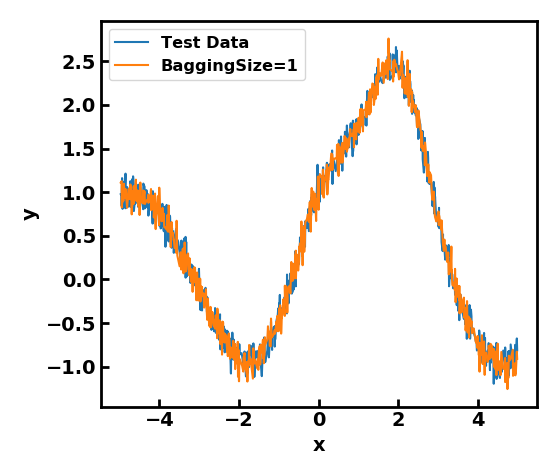
\includegraphics[width=1\linewidth]{../figures/statisticalLearning/treeMethods/BaggingTreeRegressorExampleOneTree}
		\caption{Bagging tree regressor result with one tree.}
	\end{subfigure}\quad
	\begin{subfigure}[b]{0.42\textwidth}
		\centering
		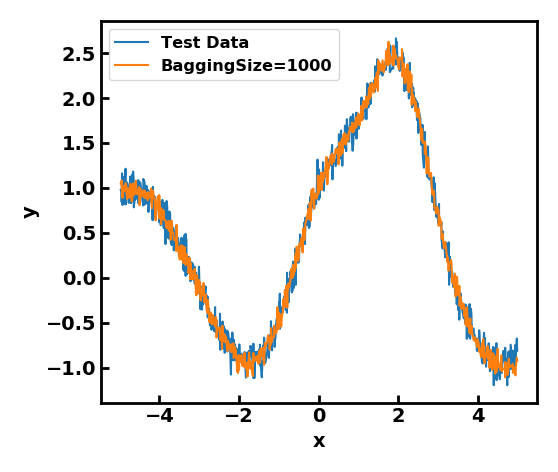
\includegraphics[width=1\linewidth]{../figures/statisticalLearning/treeMethods/BaggingTreeRegressorExampleOneThousandTrees}
		\caption{Bagging tree regressor result with 1000 trees.The predictions from 1000 trees are less oscillated. }
	\end{subfigure}\quad
	\begin{subfigure}[b]{0.42\textwidth}
		\centering
		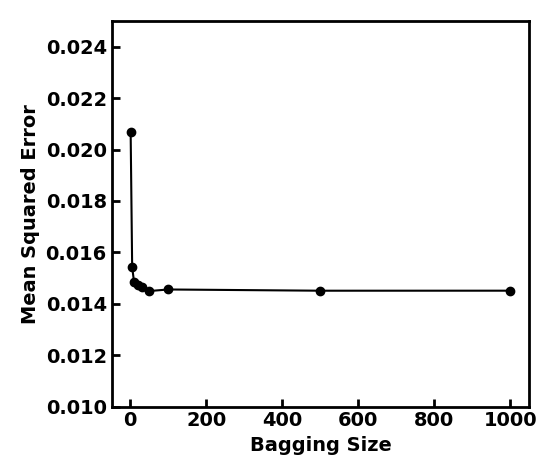
\includegraphics[width=1\linewidth]{../figures/statisticalLearning/treeMethods/BaggingTreeRegressorExampleAccuracy}
		\caption{Mean squared error as a function of bagging size. The intrinsic error is 0.01.}
		\label{fig:BaggingTreeRegressionDemo}
	\end{subfigure}
	\caption{Demonstration of a bagging tree regressor. The training and testing data set are generated by $y = \exp(-x^2) + 1.5\exp(-(x-2)^2) + sin(x) + \epsilon, \epsilon\sim N(0,0.01)$. Code: treeBaggingRegressorExample.py}
\end{figure}


\subsection{Random Forest and Extra tree}

The main difference between random forests and extra trees (usually called extreme random forests) lies in the fact that, instead of computing the locally optimal feature/split combination (for the random forest), for each feature under consideration, a random value is selected for the split (for the extra trees).

This leads to more diversified trees and less splitters to evaluate when training an extremly random forest.





\subsubsection{Summary}


\begin{remark}[on number of tree chosen]
	In general, the more trees you use the better get the results. However, the improvement decreases as the number of trees increases, i.e. at a certain point the benefit in prediction performance from learning more trees will be lower than the cost in computation time for learning these additional trees.
	Random forests are ensemble methods, and you average over many trees. Similarly, if you want to estimate an average of a real-valued random variable (e.g. the average heigth of a citizen in your country) you can take a sample. The expected variance will decrease as the square root of the sample size, and at a certain point the cost of collecting a larger sample will be higher than the benefit in accuracy obtained from such larger sample.
	
	In your case you observe that in a single experiment on a single test set a forest of 10 trees performs better than a forest of 500 trees. This may be due to statistical variance. If this would happen systematically, I would hypothesize that there is something wrong with the implementation.
	Typical values for the number of trees is 10, 30 or 100. I think in only very few practical cases more than 300 trees outweights the cost of learning them (well, except maybe if you have a really huge dataset).	
\end{remark}





\subsection{Tree boosting}



\begin{algorithm}[H]
	\SetAlgoLined
	\KwIn{Initial guess $x_0$,  training data set $(x_1,y_1), (x_2,y_2),...,(x_N,y_N)$, tree maximum-depth $D$, and number of trees $B$.}
	Set $k = 0$. \\
	Set $\hat{f}(x) = 0$ and initial residual $r_i^{(0)} = y_i, i=1,2,...,N$.
	\Repeat{ k = B}{
		Fit a tree $\hat{f}^b$ with maximum depth $D$ to the training data $(x_1,y_1), (x_2,y_2),...,(x_N,y_N)$.\\
		Update $\hat{f}$ by 
		$$\hat{f} = \hat{f} + \hat{f}^b.$$\\
		Update the residual
		$$r_i = y_i - \hat{f}(x_i) = r_i - \hat{f}^b$$\\
		Set $k = k + 1$\\
	}
	\KwOut{the boosted model $\hat{f}$.}
	\caption{Boost regression tree}
\end{algorithm}


\begin{remark}
	Reference \cite[322]{james2013introduction}.
\end{remark}

\begin{remark}[training parameters]\hfill
	\begin{itemize}
		\item The number of trees $B$. If $B$ is too large, then it tends to overfit. We can use cross-validation to select $B$.
		\item The learning parameter $\lambda$. Small $\lambda$ will learn slowly and require a large $B$.
		\item The maximum depth $D$ of each tree, which controls the complexity of the boosted ensemble.  
	\end{itemize}
\end{remark}



\subsection{Gradient tree boosting }

\begin{algorithm}[H]
	\SetAlgoLined
	\KwIn{Initial guess $f_0(x) = \arg\min_{\gamma} \sum_{i=1}^N L(y_i,\gamma)$}.\\
	Set $m = 1$. \\
	\Repeat{ m = M}{
		For $i=1,2,...,N$ compute
		$$r_{im} = -\frac{\Pa L(y_i,f(x_i))}{\Pa f(x_i)}_{f = f_{m-1}}$$\\
		Fit a regression tree to the targets $r_{im}$ givin terminal regions $R_{jm},j=1,2,...,J_m$\\
		For $j=1,2,...,J_m$, compute
		$$\alpha_{jm} = \arg\min_{\alpha} \sum_{x_i\in R_{jm}} L(y_i,f_{m-1}(x_i) + \gamma).$$\\
		Update $f_m(x) = f_{m-1}(x) + \sum_{j=1}^{J_m} \alpha_{jm} I(x\in R_{jm})$.\\
	}
	Construct the boosted model,
	$$\hat{f}(x) = f_M$$\\
	\KwOut{the boosted model}
	\caption{Gradient Regression Tree Boosting Algorithms}
\end{algorithm}


\begin{remark}[interpretation]\hfill
	\begin{itemize}
		\item The initial $f_0$ is a constant that minimizes the loss function.
		\item 
	\end{itemize}
\end{remark}


\begin{remark}[common choice of loss functions]
	
\end{remark}


\subsubsection{Comparison of different ensemble methods}


\subsection{Summary}

\begin{itemize}
	\item  In Bagging, each individual trees are independent of each other because they consider different subset of features and samples.
	\item In bagging trees, individual trees are independent of each other.
	\item Bagging method improves the performance by aggregating the results of weak learners.
\end{itemize}

\begin{itemize}
	\item In boosting trees, individual weak learners are not independent of each other.
	\item Boosting method improves the performance by aggregating the results of weak learners
\end{itemize}


\begin{itemize}
	\item Random forest is based on bagging concept, that consider faction of sample and faction of feature for building the individual trees.
	\item Since Random Forest aggregate the result of different weak learners, increasing number of trees in model will increase performance.  
	\item For comparison, bagging trees will consider a faction of samples but \textbf{all the feature} for building the individual trees.
\end{itemize}

\begin{itemize}
	\item For the hyperparameter 'max\_depth', increasing it from  certain value of depth may overfit the data.
\end{itemize}

\section{Notes on Bibliography}
For ensemble learning methods, see \cite{seni2010ensemble}.

For boosting, see \cite{schapire2012boosting}.

For gradient boost machine, see \cite{friedman2001greedy}.

\printbibliography
\end{refsection}




\begin{refsection}
\startcontents[chapters]	
\chapter{Unsupervised statistical learning}
\printcontents[chapters]{}{1}{}	

\section{Principal component analysis (PCA)}\index{Principal component analysis}\label{ch:statistical-learning:sec:PCA}
\begin{mdframed}
\textbf{general remarks}\\

\end{mdframed}

\subsection{PCA from different perspectives}
\subsubsection{Geometric approach}

\begin{definition}[geometric PCA ]\cite[19]{ma2002generalized}
Consider a set of points $\bm{X}=\{x_1,x_2,...,x_N\},x_i\in \R^D$ and assume they are lying in a low dimensional affine subspace $S$. Note that every point $x_i$ in $\bm{X}$ can be reproduced by
$$x_i = \mu + U_d y_i + \epsilon_i,$$
where $\mu \in \R^D, U_d \in \R^{D\times d}$ is a matrix with independent columns, $y_i \in \R^d$ is the linear combination coefficients, and $\epsilon_i\in \R^D$ is the model error. 
The goal principal component analysis is to find $\mu,U_d,\{y_i\}$ such that the sum of squared errors is minimized.
\end{definition}

\begin{remark}[redundancy in the representation]\cite[19]{ma2002generalized}\hfill
\begin{itemize}
	\item They are redundancy in the above representation because of the arbitrariness in the choice of $\mu$ and $U$. For example, $x_i = \mu + U_dy_i = (\mu + U_dy_0) + U_d(y_i - y_0)$. We can remove this translational ambiguity by requiring $\mu = \frac{1}{N}\sum_{i=1}^N x_i$; therefore we are effectively dealing with demeaned data. 
	\item Another ambiguity is due to the arbitrariness in the choice of basis spanning the subspace. We can remove this ambiguity by enforcing orthonormality in the columns of $U_d$. 
\end{itemize}	
\end{remark}



\begin{lemma}[geometric PCA in the optimization framework]
Consider a set of points $\bm{X}=\{x_1,x_2,...,x_N\},x_i\in \R^D$ and further assume they are demeaned such that $\frac{1}{N}\sum_{i=1}^N x_i = 0$. 
\begin{itemize}
	\item Then finding $d$ orthonormal basis (i.e. $U_d$) and $y_i, i=1,...,N$ that minimizes the sum of squared errors is given by		
	$$\min_{U_d, \{y_i\}} \norm{X-UY}^2_F = \sum_{i=1}^N \norm{x_i - U_dy_i}^2, s.t., U^TU = I_d.$$
	\item The necessary condition for $y_i, i=1, ..., N$ to achieve optimality is
	$$\hat{y}_i = U^Tx_i.$$
	\item The optimization problem can be alternatively formulated as
	$$\min_{U_d} \norm{X-UU^TX}^2_F, s.t., U^TU = I_d.$$
\end{itemize}
\end{lemma}
\begin{proof}
The Lagrangian function is given by
$$L = \sum_{i=1}^{N}\norm{x_i - U_dy_i}^2 + Tr((I_d - U^TU)\Lambda),$$
where $\Lambda\in \R^{d\times d}$ is the matrix of Lagrange multipliers. Then we have
$$\frac{\Pa L}{\Pa y_i} = 0 \implies -2U^T_d(x_i - U_dy_i) = 0 \implies y_i = U^T_dx_i,$$
where we use the fact that $U^T_dU_d = I_d$.
\end{proof}


\begin{theorem}[PCA via SVD]
\cite[21]{ma2002generalized}Let $X = [x_1,x_2,...,x_N] \in \R^{D\times N}$ be the data matrix. Let $X = U\Sigma V^T$ be the singular value decomposition (SVD) of $X$. Then for any given $d < D$, a solution to PCA is the first $d$ columns of$U$, given as $U_d = [u_1,u_2,...u_d]$ and $\{y_i\}$ is the top $d\times N$ sub matrix $\Sigma_d V_d^T$ of the matrix $\Sigma V^T$ (each column of length $d$ is one $y_i$ and in $y_i$ each row is scaled in $\sqrt{\lambda_i}$). 
\end{theorem}
\begin{proof}
\begin{align*}
    \norm{X - UU^TX}^2_F &= Tr((X - UU^TX)^T(X - UU^TX))\\
            &=Tr(X^TX) - Tr(XUU^TX) - Tr(UU^TX^TX) + Tr(X^TUU^TUU^TX)\\
            &=Tr(X^TX) - 2Tr(XUU^TX) + Tr(X^TUU^TX)\\
            &=Tr(X^TX) - Tr(X^TUU^TX)\\
\end{align*}
Note that
$Tr(XUU^TX) = Tr(U^TXX^TU) = \sum_{i=1}^d u_i^T XX^T u_i$.
From Rayleigh quotient theorem (\autoref{ch:linearalgebra:th:Raylleighquotient}), we know that maximum of $Tr(U^TXX^TU$ is attained when $u_i$ are the top $d$ eigenvectors. 
\end{proof}

\begin{remark}[PCA, rank approximation, and SVD]
	Let $X$ be the data matrix $X\in \R^{p\times N}$. Let $X$ has SVD given by $X=\sum_{i=1}^d \sigma_i u_iv_i^T$. Then \textbf{if $X$ is demeaned}, the principal component vectors of $X$ are given by $u_1,...,u_d$ and the projection coordinates are $\sigma_i v_i^T$.
	However, if $X$ is not demeaned, the principal components and SVD are not related.
\end{remark}

\begin{remark}[kernelizing PCA]\cite[142]{shawe2004kernel}\hfill
\begin{itemize}
    \item Note that in the kernel PCA, we only have access to $X^TX$, instead of $XX^T$, therefore, we can \textbf{only directly calculate the projected coordinates (projection into the eigenspace), and cannot calculate the eigenvector.}
    \item However, we can still project new data point via the following dual form method. 
\end{itemize}
\end{remark}






\begin{lemma}[projection of new data points, primal form]
Given given a new input data $x\in \R^D$ (assuming it is sampled from a distribution has zero mean), we can find its coordinates in the subspace given as $U_d^T x = [u_1^Tx,u_2^Tx,...,u_d^Tx]^T$.
\end{lemma}


\begin{lemma}[projection of new data points, dual form]
From the working mechanism of $SVD$, we know that eigenvectors in $U$ and $V$ are related.
The eigenvector $u_i = Xv_i/\sqrt{\lambda_i} = X\alpha_i$, and then the projection a new data point will have coordinate in the subspace given as
$[\alpha_i^T X^Tx]$
\end{lemma}


\subsubsection{Statistical approach: random vectors}
\begin{definition}[PCA for random vectors]
Given a \textbf{zero mean}  random  vector $X\in \R^D$ with covariance matrix $\Sigma_X$.  The PCA problem is that we want to find $d$ unit principle components $u_i,u_i\in \R^D, i=1,2,...,d$ such that 
\begin{itemize}
	\item random variable $y_i = u_i^T X, i=1,2,...,D$ are uncorrelated to each other; that is
	$$cov(y_i,y_j) = u_i^TCov(X,X)u_i = u_i^T\Sigma_X u_i;$$
	\item the variances of $y_1,...y_D$ are decreasing. 
\end{itemize}

Mathematcially, we have
\begin{align*}
    u_1 &= \arg \max u^T\Sigma_X u, ~s.t.~  u^Tu = 1  \\
    u_2 &= \arg \max u^T\Sigma_X u, ~s.t.~ u^Tu=1, u^Tu_1 = 0\\
    \dots &  \\
    u_2 &= \arg \max u^T\Sigma_X u, ~s.t.~ u^Tu=1, u^Tu_1 = 0
\end{align*}
\end{definition}

\begin{theorem}
The solution to the PCA problem in the statistical approach is given by the top $d$ eigenvectors of $\Sigma_X$.
\end{theorem}
\begin{proof}
(1) Use Reyleigh quotient theorem (\autoref{ch:linearalgebra:th:Raylleighquotient}) and quadratic form maximization theorem (\autoref{ch:linearalgebra:th:MaximizingQuadraticFormsOnUnitSpheres}). 
\end{proof}


\begin{remark}[implications]
The statistical point of view enables to construct a new random variable that exhibits the most significant variations. Such new random variable can be further used in classification, regression and optimal control.
\end{remark}

\subsubsection{Statistical approach: random samples}
\begin{definition}[PCA for random vectors]
	Given a set of multi-dimensional random samples $x_1,...,x_N\in \R^D$ with covariance matrix $\Sigma_X$.  The PCA problem is that we want to find $d$ unit principle components $u_i,u_i\in \R^D, i=1,2,...,D, U=[u_1,...,u_D]$ such that 
	\begin{itemize}
		\item the sample covariance matrix $\Sigma_y$ of $y_1,...,y_N$ are diagonal;
		\item the diagonal terms in $\Sigma_y$ are decreasing. 
	\end{itemize}
	
	Mathematically, we have
	\begin{align*}
	u_1 &= \arg \max u^T\Sigma_X u, ~s.t.~  u^Tu = 1  \\
	u_2 &= \arg \max u^T\Sigma_X u, ~s.t.~ u^Tu=1, u^Tu_1 = 0\\
	\dots & \\
	u_2 &= \arg \max u^T\Sigma_X u, ~s.t.~ u^Tu=1, u^Tu_1 = 0
	\end{align*}
\end{definition}

\begin{theorem}
	The solution to the PCA problem in the statistical approach is given by the top $d$ eigenvectors of $\Sigma_X$.
\end{theorem}
\begin{proof}
	(1) Use Reyleigh quotient theorem (\autoref{ch:linearalgebra:th:Raylleighquotient}) and quadratic form maximization theorem (\autoref{ch:linearalgebra:th:MaximizingQuadraticFormsOnUnitSpheres}). 
\end{proof}


\begin{remark}[implications]
	The statistical point of view enables construction a new random variable that exhibits the most significant variations. Such new random variable can be further used in classification, regression and optimal control.
\end{remark}



\begin{remark}[rank deficiency for high dimensional input data]
When the input data $x_i \in \R^D$ is high dimensional such that $D\gg N$, the scattering matrix 	
	$$S^2 = \sum_{i=1}^N (x_i - \mean{x})(x_i - \mean{x})^T,$$
will have rank at most $N-1$ (when columns are linearly independent) or smaller (when there are linearly dependent columns). 	
\end{remark}





\subsection{Properties of PCA}
\subsubsection{Representation in principle component space}

\begin{lemma}[representation in the principal component space]
Let $X = [x_1,x_2,...,x_N] \in \R^{D\times N}$ be the data matrix. Let $X = U\Sigma V^T$ be the singular value decomposition (SVD) of $X$. 
\begin{itemize}
	\item Then the coordinate vector of $x_i$ in the basis of $U\in \R^{D\times p}$ is given by
	$$y_i = U^Tx_i, y_i\in \R^p.$$
	\item The matrix $P=UU^T$ is an orthonormal projection matrix that projects a vector in $\R^D$ to a subspace $S\subseteq \R^D$, where $S$ has the basis $U$. We have recovery representation
	$$Uy_i = UU^Tx_i = x_i.$$
	\item If $X$ has $D$ independent columns, then $U\in \R^{D\times D}$, then $P = I$
\end{itemize}
\end{lemma}
\begin{proof}

(2) Since $X = U\Lambda V^T$, then $x_i \in S$. ($x_i$ can be written as a linear combination of columns vectors of $U$, and the coefficients are the $i$ column of the matrix $\Lambda V^T$). Therefore $x_i = Px_i$. 	
\end{proof}


\subsubsection{Distance preserving properties}


\begin{theorem}[distance preserving properties]
	Let $X = [x_1,x_2,...,x_N] \in \R^{D\times N}$ be the data matrix. Let $X = U\Sigma V^T$ be the singular value decomposition (SVD) of $X$. For each data point $x_i$. Let $y_i = U^Tx_i = x_i$ be the (new) coordinates projected on the eigen-basis. 
It follows that
\begin{itemize}
	\item (total distance preservation)
	$$\norm{y_i' - y_j'}^2 = \norm{x_i - x_j}^2.$$
	\item (total distance along principal component $k$ )  
	$$ \sum_{i=1}^N (u_k^Tx_i)^2 = \sigma_k^2.$$
	\item (total distance)  
	$$ \sum_{i=1}^N x_i^Tx_i = \sum_{k=1}^D \sigma_k^2.$$
\end{itemize}
\end{theorem}
\begin{proof}
(1)
\begin{align*}
\norm{y_i' - y_j'}^2 &= (y_i - y_j)^T(y_i-y_j) \\
					 &= (U^Tx_i-U^Tx_j)^T(U^Tx_i-U^Tx_j)\\
					 &= (x_i-x_j)^TUU^T(x_i-x_j)\\
					 &= (x_i-x_j)^T(x_i-x_j)
\end{align*}	
where we used the factor that $x_i, x_j, x_i-x_j$ are all lying inside the subspace $S$ spanned by $U$, and the orthogonal projection matrix to $S$ is $P=UU^T$. Therefore $P(x_i-x_j) = (x_i-x_j)$. 
(2)
\begin{align*}
\sum_{i=1}^N (u_k^Tx_i)^2 &= u_k^T(\sum_{i=1}^N x_ix_i^T) u_k \\
                          &= u_k^T XX^T u_k \\
                          &= u_k^T U\Sigma^2 U^T u_k \\
                          &= \sigma_k^2 
\end{align*}
(3) Note that $$ \sum_{i=1}^N x_i^Tx_i = \sum_{i=1}^N \sum_{k=1}^D (x_i^Tu_k)^2.$$
Then we use (2).
\end{proof}

\subsubsection{Variance preserving properties}

\begin{lemma}[PCA variance preserving property]\label{ch:statistical-learning:th:PCAVariancePreservingProperty}
Let $x_1,x_2,...,x_N \in \R^{D}$ be a set of random samples.
Define total variance and scatter matrix as
$$\Delta^2 = \sum_{i=1}^N (x_i - \mean{x})^T(x_i - \mean{x}),$$	
$$S^2 = \sum_{i=1}^N (x_i - \mean{x})(x_i - \mean{x})^T.$$
Denote the eigenvalue decomposition as
$$S^2 = U\Lambda U^T,$$
and the projected samples $y_i = U^Tx_i$. 
It follows that 
\begin{itemize}
	\item $$\Delta^2 = \Delta^2_U = \sum_{i=1}^N (y_i - \mean{y})^T(y - \mean{y}).$$
	
	\item The variance of projected coordinates on the subspace spanned by $V=[u_1,...,u_j]$ is
	$$\sum_{i=1}^N (V^Tx_i - V^T\mean{x})^T(V^Tx_i - V^T\mean{x}) = \lambda_1+\lambda_2+ \cdots \lambda_j.$$
	\item $$\Delta^2 = \lambda_1+\lambda_2+ \cdots \lambda_D.$$
\end{itemize}
\end{lemma}
\begin{proof}
(1)	
\begin{align*}
\sum_{i=1}^N (y_i - \mean{y})^T(y_i - \mean{y}) &= \sum_{i=1}^N (U^Tx_i - U^T\mean{x})^T(U^Tx_i - U^T\mean{x}) \\
&= \sum_{i=1}^N (x_i - \mean{x})^TUU^T(x_i - \mean{x})\\
&=  \sum_{i=1}^N (x_i - \mean{x})^T(x_i - \mean{x})\\
&= (x_i-x_j)^T(x_i-x_j)
\end{align*}	
where we used the factor that $x_i, x_j, \mean{x}$ are all lying inside the subspace $S$ spanned by $U$, and the orthogonal projection matrix to $S$ is $P=UU^T$. Therefore $P(x_i-\mean{x}) = (x_i-\mean{x})$.
(2)(3)
\begin{align*}
 & \sum_{i=1}^N (V^Tx_i - V^T\mean{x})^T(V^Tx_i - V^T\mean{x}) \\
&= \sum_{i=1}^N (x_i - \mean{x})^TVV^T(x_i - \mean{x})\\
&= \sum_{i=1}^N Tr((x_i - \mean{x})^TVV^T(x_i - \mean{x}))\\
&= \sum_{i=1}^N Tr(VV^T(x_i - \mean{x})(x_i - \mean{x})^T)\\
&=  Tr(VV^T\sum_{i=1}^N(x_i - \mean{x})(x_i - \mean{x})^T)\\
&= Tr(VV^T S^2) \\
&= Tr(V^TU\Lambda U^TV) \\
&= \lambda_1+\lambda_2+ \cdots \lambda_j
\end{align*} 	
where we use matrix trace cyclic property (\autoref{appendix:th:matrixtraceproperty}) and block matrix property (\autoref{appendix:SumVectorProductToMatrixProduct})
$$\sum_{i=1}^N(x_i - \mean{x})(x_i - \mean{x})^T = S^2.$$
\end{proof}


\subsubsection{PCA and data processing}

\begin{remark}
Let $X = [x_1,x_2,...,x_N] \in \R^{D\times N}$ be the data matrix.	
\begin{itemize}
	\item In general, add a constant vector $c\in \R^D$ will not change the principal components vectors as we require data matrix to be demeaned before conducting SVD or eigendecomposition. However, SVD on original matrix $X$ and the shifted matrix $X'$ will yield different results.
	\item Assume $X$ is demeaned and its SVD is given by
	$X=\sum_{i=1}^d \sigma_i u_iv_i^T$.
	\begin{itemize}
		\item Let $X' = cX, c\in \R$. Then uniformly scaling the original data matrix will not change its principal components; it will only scale its singular value/ eigenvalues.
		\item Suppose we scale each sample by $c_i, i = 1,...,N$. Then the SVD results will completely change.
		\item Suppose we scale each components by $c_i, i=1,...,D$. Then the SVD for the new data matrix is given by
		$$X' = \sum_{i=1}^d c_i\sigma_i u_iv_i^T.$$
		That is, the principal components will not change, but the singular values/eigenvalues will change.  
	\end{itemize}
\end{itemize}

\end{remark}





\subsection{Probabilistic PCA}

\begin{remark}[motivations] PCA have several limitations:
\begin{itemize}
	\item Non-parametric and no probabilistic model for observed data.
	\item The variance-covariance matrix needs to be
	calculated, which can be very computation-intensive for large datasets
	with a high dimensions.
	\item  Does not deal properly with missing data. Incomplete data must either be discarded or imputed	using ad-hoc methods
	\item Outlying data observations can unduly affect the
	analysis
\end{itemize}	

Probabilistic PCA has several advantages:
\begin{itemize}
	\item Addresses limitations of regular PCA.
	\item PCA can be used as a general Gaussian density model
	in addition to reducing dimensions.
	\item Maximum-likelihood estimates can be computed for
	elements associated with principal components.
	\item Captures dominant correlations with few parameters.
	\item Multiple PCA models can be combined as a probabilistic mixture.
	\item Can be used as a base for Bayesian PCA
\end{itemize}	
\end{remark}

\begin{definition}
	

\begin{itemize}
	\item $y \sim Wx + \mu + \epsilon$, where $X\in MN(0, I), \epsilon\sim MN(0, \sigma^2 I), \mu\in \R^n$.
	\item $Y \sim MN(\mu, C_Y), C_Y = WW^T + \sigma^2 I$
\end{itemize}	
	
	
\end{definition}

\begin{remark}[interpretation]\hfill
\begin{itemize}
	\item Probabilistic PCA can be viewed a latent factor model with $X$ being the latent variable. 
	\item Normal PCA is a limiting case of probabilistic PCA, taken as
	the limit as the covariance of the noise becomes infinitesimally
	small ($\sigma^2 \to 0$). 
\end{itemize}	
	
\end{remark}

\begin{theorem}[parameter estimation in probabilistic PCA]
	
\end{theorem}


\section{Robust PCA}
\subsection{Robust PCA with outliers}
\subsubsection{Iteratively reweighted least square method}
\begin{algorithm}[H]
	\SetAlgoLined
	\KwIn{Data matrix $X\in\R^{D\times N}$, dimension $d$, and parameter $\epsilon_0>0$}
	Initialize low dimensional subspace $U$, mean vector $\mu$, and projection $Y$ from canonical PCA.\\
	\Repeat{convergence of $\mu 1^T + UY$}{
	$\epsilon_j = \norm{x_j - \mu - Uy_j}_2, w_j = \frac{\epsilon_0^2}{\epsilon_0^2+\epsilon_j^2}$\\
	Construct weighted mean and scatter matrix 
	$$\mu = \frac{\sum_{j=1}^N w_j(x_j - Uy_j)}{\sum_{j=1}^N w_j}, \Sigma = \frac{\sum_{j=1}^N w_j(x_j - \mu)(x_j-\mu)^T}{\sum_{j=1}^N w_j}$$	\\
	Calculate the top eigenvectors $U$ of $\Sigma$.\\
	$$Y = U^T(X-\mu 1^T)$$\\
	}
	
	\KwOut{The low dimensional subspace $U,Y,\mu$}
	\caption{Iterative reweighted least square PCA with outliers algorithm}
\end{algorithm}

\begin{remark}
	Reference \cite[105]{vidal2016generalized}.
\end{remark}

\begin{remark}[interpretation]
The weights of outliers are adjusted to smaller value relative to weights of inliers.
\end{remark}


\subsubsection{Random sample consensus(RANSAC) method}

\begin{algorithm}[H]
	\SetAlgoLined
	\KwIn{Data set $\cX$ consists of $x_1,x_2,...,x_N, x_i\in \R^D$, maximum number of iterations $k$, threshold on fitting error $\tau$, threshold on minimum number of inliers $N_{min}$}
	Initialize $i=0$\\
	\Repeat{i = k}{
		Get subsample $cX_i$ from $\cX$.\\
		Construct the subspace $U_i$ by using PCA on $\cX_i$.\\
		Find out $\cX_{inlier} = \{x\in\AA: dist(x,U_i)\leq \tau \}.$\\
		If $\abs{\cX_{inlier}} \geq N_{min}$, break.\\
		
		Set $i=i+1.$\\
	}
	\KwOut{The estimated subspace $U_i$}
	\caption{Random sample consensus PCA with outliers algorithm}
\end{algorithm}

\begin{remark}
	Reference \cite[107]{vidal2016generalized}.
\end{remark}

\begin{lemma}[random sample property]\cite[508]{vidal2016generalized}
Assume the given $N$ data points contain $p$ portion inliers and $1-p$ portion of outliers. We need to sample $k$ points with replacement to estimate the model.
\begin{itemize}
	\item In one sample of size $k$, the probability that all $k$ samples are inlier is $p^k$.
	\item In $m$ trials, the probability that there is at least one sample are all inliers is $1 - (1 - p^k)^m$.
	\item The number of trials needed to guarantee the probability of at least one trial samples are all inliers is at least $q$ is
	$$m\geq \frac{\log(1-q)}{\log(1-p^k)}$$
\end{itemize}
\end{lemma}
\begin{proof}
Straight forward.
\end{proof}

\begin{remark}[interpretation]
This lemma gives an estimate of how many iterations the algorithm needs to run.
\end{remark}

\begin{remark}[RANSAC is tolerant to outliers]
RANSAC usually can tolerate up to 50 percent of outliers.
\end{remark}






\section{Non-negative matrix factorization}

\begin{definition}[Non-negative matrix factorization, NMF]\cite{lee1999learning}\index{non-negative matrix factorization}
Let $X$ be the data matrix partitioned as $X=[x^(1),x^(2),...,x^(N)],x^(i)\in \R^p$, the non-negative matrix factorization problem is to 
$$\min_{F_{ij}\geq 0, G_{ij}\geq 0} \norm{X-FG}^2_F$$
where $F\in \R^{p\times k}, G\in \R^{k\times N}$
\end{definition}

\begin{remark}[interpretation]\hfill
\begin{itemize}
    \item In the ideal case, we want to decompose each data vector as the 'additive'/positive linear combination of $k$ basis vectors(in each column of $F$), given as
        $$x^(i)_{j} = \sum_{m=1}^k F_{jm}G_{mi}$$
    and each column of $G$ is the loading/coefficient for the $k$ basis.
    \item Usually $p \gg k$ such that we can learn low dimension representations.
\end{itemize}
\end{remark}


\begin{remark}[NMF vs. PCA]\hfill
\begin{itemize}
    \item PCA can also be viewed a decomposition of each data vector as linear combination of $k$ basis vectors, given as
    $$x^(i)_{j} = \sum_{m=1}^k U_{jm}\sigma_mV_{mi}$$
    where $X = U\Sigma V$ is obtained from SVD. And the order of the basis are sorted based on importance. 
    \item PCA allows negative coefficients and basis vectors can cancel with each other.
    \item PCA basis vectors are usually used for NMF initialization.
\end{itemize}
\end{remark}






\section{Manifold learning}
\subsection{Kernel PCA}\index{kernel PCA}


\begin{algorithm}[H]
\SetAlgoLined
\KwIn{Data set consists of $x_1,x_2,...,x_N, x_i\in \R^D$}
 Define a semi-positive symmetric kernel $k(x,y)$ and construct a kernel matrix $K$ such that $K_{ij} = k(x_i,x_j)$ and \textbf{center} $K$;\\
 
 Compute the eigenvectors $u^i$ and eigenvalues $\lambda_i$ centered kernel matrix $K$ such
 $$Ku^i = \lambda_i u^i$$
 
 The low dimensional coordinate $y_i \in \R^p, D\gg p$ is given as
 $$y_i=\begin{pmatrix}
        u^1_{i}\sqrt{\lambda_1}\\
        u^2_{i}\sqrt{\lambda_2}\\
        \dots\\
        u^p_{i}\sqrt{\lambda_2}\\
 \end{pmatrix}
 $$
 
 \KwOut{The low dimensional coordinate $y_i \in \R^p,i=1,2,...,N$}
 \caption{Kernel PCA algorithm}
\end{algorithm}


\begin{lemma}[\textbf{best low rank approximation to kernel matrix}]
Let $M_{ij} = \ip{y_i,y_j}$, then $M$ is the optimal solution to the low rank approximation to the kernel problem, given as
$$\min_{rank(M)=p} \norm{K-M}_F^2$$
More compactly
$$M = Y^TY,Y=[y_1,y_2,...,y_N]$$ and $M$ is the approximated kernel matrix constructed from low dimensional coordinates.
\end{lemma}
\begin{proof}
directly from the low rank approximation property of SVD. Moreover, 
$$M_{ij} = \ip{y_i,y_j} = \sum_{n=1}^p \sqrt{\lambda_n}u^n_i \sqrt{\lambda_n} u^n_j =\sum_{n=1}^p y_{in}y_{jn}$$
\end{proof}

\begin{remark}
Reference \cite[132]{vidal2016generalized}.
\end{remark}

\begin{remark}[eigendecompostion always exist]
Note that eigendecompostion always exist since $K$ is a symmetric positive definite matrix. 
\end{remark}



\begin{remark}
\textbf{PCA is a particular example of kernel PCA} with kernel being $k(x,y)=x^Ty$.
\end{remark}




\subsection{Multidimensional scaling and Isomap}
\begin{mdframed}
\textbf{General remark}:
The working mechanism of kernel PCA, Multidimensional scaling and isomap are quite similar except how the kernel is constructed. The low dimensional coordinates have the same property of approximating the kernel matrix or the distance matrix. 
\end{mdframed}


\begin{definition}[distance matrix associated with a set of points]\cite[398]{borg2005modern}
Consider a set of $N$ points $z_1,z_2,...,z_N \in \R^M$. The \textbf{distance matrix} $D\in \R^{N\times N}$ associated with the data $z$s is defined by $$D_{ij} = \norm{z_i-z_j} =\sqrt{ z_i^Tz_i - 2z_i^Tz_j + z_j^Tz_j}.$$
\end{definition}





\begin{definition}[multidimensonal scaling problem]\index{multidimensional scaling}
Consider a set of $N$ points $z_1,z_2,...,z_N \in \R^M$ and its associated distance matrix $D\in \R^{N\times N}$.  The goal of the multidimensional scaling problem is to find a set of low-dimensional representation of $y_1,y_2,...,y_N, y_i\in \R^D, D\ll M$ for $z$s such that we maximally preserving the distance matrix:
$$\min_{Y} \norm{D_Y - D}_F^2$$
where $D_Y$ is the distance matrix from lower dimensional representation $Y$.
\end{definition}

\begin{remark}
The MDS problem does not have analytical solutions and require iterative method to solve it. 
Another way to solve MDS problem is to convert distance matrix matrix to inner product matrix and minimize the reconstruct inner products.
\end{remark}


\begin{lemma}[The distance matrix to inner product conversion operator]\cite[398]{borg2005modern}\hfill
\begin{itemize}
	\item Given a distance matrix $D\in \R^{N\times N}$ where $D_{ij} = \norm{z_i-z_j} =\sqrt{ z_i^Tz_i - 2z_i^Tz_j + z_j^Tz_j}$, then the operator $\tau$ defined as $$\tau(D) = Y -\frac{1}{2}HSH,$$ 
	where $Y_{ij} = (z_i - \mean{z})^T(z_j - \mean{z})$, known as \textbf{centered inner product matrix}, and $H_{ij} = \delta_{ij} - 1/N,S_{ij}=D_{ij}^2.$
	\item The distance matrix is invariant to translation and rotation. 
	The centered inner product matrix is invariant to translation and rotation.
\end{itemize}	

\end{lemma}
\begin{proof}
It can be showed that
$$D_{ij}^2=z_i^2+z_j^2-2z_iz_j$$
$$\frac{1}{N}\sum_{i}^n D_{ij}^2 = \sum_i z_i^2/n + z_j^2 - 2z_j\mean{z}$$
$$\frac{1}{N}\sum_{j}^n D_{ij}^2 = z_i^2 + \sum_j z_j^2/n - 2z_i\mean{z}$$
$$\frac{1}{N^2}\sum_{i}^n\sum_{j}^n D_{ij}^2 = \sum_iz_i^2/n + \sum_jz_j^2/n - 2\mean{z}\mean{z}$$
The centered inner product $Y_{ij}$ has
$$Y_{ij}=z_iz_j - z_j\mean{z} - z_i\mean{z} +\mean{z}\mean{z}$$
then we have
\begin{align*}
Y_{ij} = -\frac{1}{2}(D_{ij}^2 - \frac{1}{n}\sum_{j}^n D_{ij}^2)-\frac{1}{n}\sum_{j}^n D_{ij}^2-
+\frac{1}{n^2}\sum_{i}^n\sum_{j}^n D_{ij}^2
\end{align*}
\end{proof}


\begin{definition}[MDS in alternative inner product matrix form]
The Multidimensonal scaling problem:
Given a distance matrix/dissimilarity measure matrix $D\in \R^{N\times N}$, the goal is to find a matrix $Y=[y_1,y_2,...,y_N], y_i\in \R^D$ ($Y_i$ is usually lower dimensional) to maximally preserving the distance/dissimilarity:
$$\min_{Y} \norm{\tau(D_Y) - \tau(D)}_F^2$$
where $D$ is the distance matrix from lower dimensional representation $Y$, $\tau$ is the distance matrix to centered inner product matrix operator.
\end{definition}


\begin{theorem}[Solution to MDS via SVD]
Given a MDS problem in inner product matrix form, the optimal solution is $$y_{ij} = \sqrt{\sigma_j}U_{ij},i=1,2,...N,j=1,2...,D$$
where $\tau(D) = U\Sigma U^T$ from SVD.
\end{theorem}
\begin{proof}
Directly from the low rank approximation property of SVD(\autoref{ch:linearalgebra:th:SVDFrobeniusnormlowrankapproximation}).
\end{proof}


\begin{remark}[explicit feature map is not available]
Note that since directly construct low dimensional embeddings from the kernel matrix, the explicit feature map $\phi: \R^p \to \R^D $ is not available.
\end{remark}

\begin{remark}[Euclidean MDS cannot capture nonlinear structure]\hfill
\begin{itemize}
\item When use Euclidean distance in the MDS, large distances and small distances are weighted equally. And note that large distances between data points provide little information on the global structure of the data set compared to small distances between neighboring data points. 
\item When use different distance measure, we can make MDS for nonlinear structure; For example, in isomap, we use geodesic distance between data points as distance measure. 
\end{itemize}
\end{remark}


\subsection{Isomap}
\begin{definition}[Isomap cost function]\cite{tenenbaum2000global}\label{}
The Isomap cost function minimization problem is
$$\min_{Y} \norm{\tau(D_G) - \tau(D_Y)}^2_F$$
where $D_G$ is the distance matrix calculated using shortest path, $Y = [y_1,...,y_N],y_i\in \R^D$ is the low dimensional embedding vector, $D_Y$ is the distance matrix from $Y$.
\end{definition}


\begin{lemma}\label{ch:statistical-learning:th:SVDsolutiontoIsomap}
The Isomap cost function minimization problem can be use SVD, that is
$$y_{ij} = \sqrt{\sigma_j}U_{ij},i=1,2,...N,j=1,2...,D$$
where $\tau(D_G) = U\Sigma U^T, \tau(D_G)\in \R^{N\times N}, U\in \R^{N\times D}, \Sigma \in \R^{D\times D}$ from SVD for symmetric matrix; that is, each row represents one low dimensional representation.
\end{lemma}
\begin{proof}
Directly from the low rank approximation property of SVD(\autoref{ch:linearalgebra:th:SVDFrobeniusnormlowrankapproximation}).
\end{proof}


\begin{algorithm}[H]
	\SetAlgoLined
	\KwIn{Data set consists of $x_1,x_2,...,x_N$}
	Construct a distance matrix $D_G$ based on geodesic distance(shortest path distance in graphs).\\
	
	Solve the Isomap cost function minimization problem
	$$\min_{Y} \norm{\tau(D_G) - \tau(D_Y)}^2_F$$ using SVD(\autoref{ch:statistical-learning:th:SVDsolutiontoIsomap})\\

	
	\KwOut{the low dimensional coordinates $y_1,...,y_N\in\R^D$.}
	\caption{Isomap algorithm}
\end{algorithm}


\subsection{Laplacian eigenmap}




\begin{definition}[Laplacian matrix]\index{Laplacian matrix}
Let $W\in \R^{N\times N}_+$ be a symmetric matrix, let $D\in \R^{N\times N}$ be a diagonal matrix with $d_{jj}=\sum_{i=1}^N w_{ij}$, then the symmetric matrix $L=D-W$ is called Laplacian matrix.
\end{definition}

\begin{lemma}[elementary property of Lapacian matrix]
\cite[140]{vidal2016generalized}\cite{von2007tutorial}Let $L$ be a Laplacian matrix, then
\begin{itemize}
    \item $L$ is positive semi-definite.
    \item The vector of all ones $\bm{1}$ is the eigenvector associated with zero eigenvalue, that is $L\bm{1} = 0$
    \item $L$ is diagonalizable but $L$ is singular matrix.
    \item $L$ has $n$ non-negative, real-valued eigenvalues $$0 = \lambda_1 \leq \lambda_2 \leq \dots \leq \lambda_n.$$
\end{itemize}
\end{lemma}
\begin{proof}
(1) Let $y\in \R^N$ be a nonzero vector, we have
$$y^TDy = \sum_{i}y^i(y_i\sum_j w_{ji})=\sum_{i}\sum_{j}y^2_i w_{ji} = \sum_{i}\sum_{j}y^2_j w_{ij}$$
$$y^TWy=\sum_{i}\sum_{j}y_iy_j w_{ij}$$
where we use the fact that $W$ is symmetric. Then we have
$$y^T(D-W)y=y^TLy = \frac{1}{2}\sum_{i}\sum_{j}w_{ij}(y_i-y_j)^2 \geq 0.$$
We can also directly prove (1) using \autoref{ch:linearalgebra:th:GerschgorinTausskytheorem}\autoref{ch:linearalgebra:th:Gerschgorintheorem}.

(2) Directly from the definition of $L$
(3) $L$ is real symmetric and therefore diagonalzable. $L$ is singular since it has eigenvalue 0.
\end{proof}  


\begin{lemma}[number of connected components from spectrum of $L$]\cite{von2007tutorial}
Let $G$ be an undirected graph with non-negative weights with Laplacian $L$. Then multiplicity $k$ of eigenvalue 0 of $L$ equals the number of connected components $A_1,...,A_k$ in the graph. The eigenspace associated eigenvalue 0 has dimensionality $k$ spanned by the indicator vectors $1_{A_1},...,1_{A_k}$ of these components.  
\end{lemma}
\begin{proof}
It is easy to show that $1_{A_1},...,1_{A_k}$ satisfy $L1_{A_i} = 0$. Note that from  \autoref{ch:linearalgebra:th:symmetricdecomposition}, we note that the geometric multiplicity is the same as the algebraic multiplicity. Therefore,  $1_{A_1},...,1_{A_k}$ will span the eigenspace. 
\end{proof}

\begin{remark}[eigenvectors]
The eigenvector calculated from software will usually be scaled version of the indicator vectors. 
\end{remark}


\begin{definition}[normalized graph Laplacian]\cite{von2007tutorial}
Given a Laplacian $L$ associated with a graph $G$, we can defined normalized Laplacian as:
\begin{itemize}
	\item $L_{sym} = D^{-1/2}LD^{-1/2} = I - D^{-1/2}WD^{-1/2}$
	\item $L_{rw} = D^{-1}L = I - D^{-1}W.$
\end{itemize}
where $D=diag(d_1,...,d_N), d_i = \sum_{ij}w_j$.
\end{definition}


\begin{remark}[connection to Markov chain transition matrix]
	The transition matrix $P$ of a Markov chain is given as
	$$P = D^{-1}W = I - L_{rw}.$$
\end{remark}


\begin{theorem}[spectrum properties of normalized Laplacian]
The normalized Laplacians satisfy the following properties:
\begin{itemize}
	\item For every $v\in \R^N$, we have
	$$v^TL_{sym}v = \frac{1}{2}\sum_{i,j} w_{ij}(\frac{v_i}{\sqrt{d_i}}-\frac{v_j}{\sqrt{d_j}}).$$
	\item $\lambda$ is an eigenvalue of $L_{rw}$ with eigenvector $u$ if and only if $\lambda$ is an eigenvalue of $L_{sym}$ with eigenvector $w = D^{1/2}u$.
	\item $\lambda$ is an eigenvalue of $L_{rw}$ with eigenvector $u$ if and only if $\lambda$ and $u$ satisfy $$Lu = \lambda Du.$$
	\item 0 is an eigenvalue $L_{rw}$ with has the eigenvector of the constant one vector $1$. 0 is an eigenvalue of $L_{sym}$ with eigenvector $D^{1/2}1$.
	\item $L_{sym}$ and $L_{rw}$ are positive semi-definite and have $n$ non-negative real-valued eigenvalues $0\leq \lambda_1\leq...\leq \lambda_n.$
\end{itemize}
\end{theorem}
\begin{proof}
Straight forward from definitions of normalized graph Laplacian.
\end{proof}
\begin{remark}[short summary]\hfill
\begin{itemize}
	\item $L_{sym}$ and $L_{rw}$ have exactly the same eigenvalues.
	\item $L$ has different nonzero eigenvalues from $L_{sym}$ and $L_{rw}$. However, they have the same number of zero eigenvalues.
\end{itemize}	
\end{remark}


\begin{corollary}[number of connected components from spectrum of $L$]\cite{von2007tutorial}
	Let $G$ be an undirected graph with non-negative weights with Laplacian $L$. Then multiplicity $k$ of eigenvalue 0 of $L,L_{sym},L_{rw}$ equals the number of connected components $A_1,...,A_k$ in the graph. The eigenspace associated eigenvalue 0 of $L,L_{rw}$ has dimensionality $k$ spanned by the indicator vectors $1_{A_1},...,1_{A_k}$ of these components. The eigenspace associated eigenvalue 0 of $L_{sym}$ has dimensionality $k$ spanned by the indicator vectors $D^{1/2}1_{A_1},...,D^{1/2}1_{A_k}$ of these components.   
\end{corollary}


\begin{definition}[The Laplacian eigenmap problem]\index{Laplacian eigenmap}\cite[140]{vidal2016generalized}
Let $x_1,...,x_N$ be the data lying on a high dimensional manifold $M$. Let $W\in \R^{N\times N}$ be the matrix such that $W_{ij}$ characterized the affinity/similarity of between the data $x$.  The Laplacian eigenmap problem is to find a low dimensional embedding $Y = [y_1,...,y_N], y_i\in \R^D$, such that if $x_i$ and $x_j$ are closed to each other, then so are $y_i$ and $y_j$. The goal is formulated as
$$\min \sum_{i,j} w_ij\norm{y_i-y_j}^2$$
with constraint $YD1 = 0$ and $YDY^T = I$. 	
\end{definition}



\begin{lemma}
	
Let $y_1,...,y_N,y_i\in \R^D$ be $N$ data vectors, the weighted distance between data vectors is given as
$$\phi(y) = \sum_{i=1}^N\sum_{j=1}^N \norm{y_i-y_j}^2w_{ij} = 2Tr(Y^TWY)$$
where $Y=[y_1,...,y^T]$
\end{lemma}
\begin{proof}
Note that if $y_i$ is scalar, then from previous lemma we see that $y^TWy = \sum_i\sum_j(y_i-y_j)^2w_{ij}$
The Trace operator is the direct counterpart.
\end{proof}


\begin{remark}[implications]
	
\end{remark}



\begin{algorithm}[H]
	\SetAlgoLined
	\KwIn{Data set consists of $x_1,x_2,...,x_N$ on a manifold $M$}
	Find the $K$ nearest neighbors of each data point $x_i,i=1,...,N$ according to some distance function $d(x_i,x_j)$ defined on $M$.\\
	Construct similarity matrix $W$, where
	$$W_{ij} = \begin{cases}
	e^{-d(x_i,x_j)^2/\sigma^2}, ~if~ i,j ~ are ~ neighbors\\
	0,~otherwise
	\end{cases}$$\\
	Construct the graph Laplacian $L = D - W$.\\
	Solve the second to top $(d+1)$ smallest generalized eigenvalues and eigenvectors of $Lu = \lambda Du$.\\
		Assign each data point $i$ with the new lower dimensional coordinate $y_i = (u_{1,i},u_{2,i},...,u_{d,i})$.\\
	
	\KwOut{The low dimensional coordinates $y_i\in \R^d, i=1,...,N$}
	\caption{Laplacian Eigenmaps algorithm}
\end{algorithm}


\begin{remark}[We ignore eigenvectors associated with zero eigenvalue]\hfill
	\begin{itemize}
		\item Note that in diffusion mapping and Laplacian eigenmap, we will ignore the top eigenvector, because the top eigenvector (the multiplicity is  1 usually)is constant 1 vector that does not provide extra information.
	\end{itemize}
\end{remark}



\subsection{Diffusion map}\index{diffusion map}
\begin{algorithm}[H]
\SetAlgoLined
\KwIn{Data set consists of $x_1,x_2,...,x_N$}
 Define a semi-positive symmetric kernel $k(x,y)$ and construct a kernel matrix $K$ such that $K_{ij} = k(x_i,x_j)$;\\
 
 Construct the diagonal matrix $D$ with $D_{jj}=\sum_{i=1}^N K_{ij}$\\
 
 Normalize each row of $K$, given as $M = D^{-1}K$;(now $M$ has the row sum 1, which is also called stochastic matrix.)
 
 Compute the second to $k+1$ largest eigenvalues and eigenvectors of $M$)\\
 
 The representation of each data point $x_i$ is the diffusion space is given as
 $$\Phi(i) = \begin{bmatrix}
 &\lambda \phi_1(i)\\ 
 &\lambda \phi_2(i)\\
 &\lambda \phi_3(i)\\
 &\dots
 \end{bmatrix}$$
 
 \KwOut{the coordinate in the diffusion space.}
 \caption{Diffusion map algorithm}
\end{algorithm}


\begin{remark}[We ignore eigenvectors associated with zero eigenvalue]\hfill
	\begin{itemize}
		\item Note that in diffusion mapping and Laplacian eigenmap, we will ignore the top eigenvector, because the top eigenvector (the multiplicity is  1 usually)is constant 1 vector that does not provide extra information.
	\end{itemize}
\end{remark}



\begin{lemma}
The transition matrix $M$ satisfying detailed balance. Moreover, we have
\begin{itemize}
	\item $M$ can be symmetrized via
	$V = \Pi M \Pi^{-1}$
	where $\Pi$ is the diagonal matrix with entries $\sqrt{\pi_1},...,\sqrt{\pi_n}$($\pi = (\pi_1,...,\pi_n)$ is the equilibrium probability vector).
	\item Let $\lambda_1,...,\lambda_n$ and $w_1,...,w_n$ be the \textbf{real eigenvalues} and unit eigenvectors of $V$. Then $M$ has the \textbf{same real eigenvalues}. The left eigenvectors of $P$ are given as
	$$\psi_j = \Pi w_j$$
	The right eigenvectors of $P$ are given as 
	$$\phi_j = \Pi^{-1} w_j$$
	\item $M$ has the following spectral decomposition:
	$$M = \sum_{k=1}^n \lambda_k \phi_k\psi_k^T = \sum_{k=1}^n \lambda_k \Pi^2\phi_k\phi_k^T$$
	\item Except for the first eigenvalue having value 1, then all other eigenvalues with their absolute value strictly less than 1.
\end{itemize}
\end{lemma}
\begin{proof}
Directly from \autoref{ch:markov-chains:th:detailedbalancechainspectrum}. 
\end{proof}


\begin{lemma}[stationary/equilibrium probability]
The stationary/equilibrium probability of the $M$ matrix is given as
$$\pi_i = \frac{d_i}{\sum_k d_k}, d_i = \sum_{j}K_{ij}$$
\end{lemma}
\begin{proof}
\begin{align*}
\pi_i &= \sum_{j}\pi_jM_{ji} \\
&= \sum_{j}\pi_j\frac{K_{ji}}{d_j} \\
& = \sum_{j} \frac{d_j}{\sum_k d_k}\frac{K_{ji}}{d_j}\\
& = \sum_{j} \frac{K_{ji}}{\sum_k d_k} = \pi_i
\end{align*}
Therefore $\pi$ is an invariant/stationary/equilibrium vector.
\end{proof}


\begin{definition}[diffusion distance]
In a Markov chain $P$ satisfying detailed balance, we can define the diffusion distance on a time step $N$ between different state $i$ and $j$ as
$$D(i,j) = \norm{P(i,\cdot) - P(j,\cdot)}^2_{1/\pi} = [\sum_k \frac{(P_{i,k} - P_{j,k})^2}{\pi_k}]^{0.5}$$
\end{definition}

\begin{remark}[interpretation]\hfill
	\begin{itemize}
		\item The distance between nodes $i,j$ is given by starting the Markov chain at each node $i,j$ let them evolve after a fixed time step and computing the mean square distance between the two resulting distributions.
		\item The distance computation is weighted by the inverse equilibrium density $1/\pi$. 
	\end{itemize}
\end{remark}

\begin{lemma}[preserving diffusion distance]\cite{de2008introduction}\cite{Holmes-Cerfon2015applied}
The diffusion distance $D(i,j)$on a time step $N$ between different state $i$ and $j$ is given as
$$[D(i,j)]^2 = \sum_{k=1}^n \lambda_k^{2} (\phi_k(i) - \phi_k(j))^2$$
where $\phi_k$ is the $k$th right eigenvector of $P$. 
In other words, the representation in Euclidean space
 $$\Phi(i) = \begin{bmatrix}
 &\lambda_1 \phi_1(i)\\ 
 &\lambda_2 \phi_2(i)\\
 &\lambda_3 \phi_3(i)\\
 &\dots
 \end{bmatrix}$$
preserves the diffusion distance.
\end{lemma}
\begin{proof}
	Note that $P_{i,j} = \sum_{k=1}^n \lambda_k \phi_k(i)\phi_k(j)\pi_k$.
	Then $$D(k,m)^2 = \sum_i\sum_j \lambda_i \phi_i(k)\phi_i(j) - \sum_i\sum_j \lambda_i \phi_i(m)\phi_i(j)$$
	where orthonormality is needed to prove.
\end{proof}


\begin{remark}[out of sample extension]
For out-of-sample extensions, see \cite{bengio2004out}\cite{laing2007coarse}.
\end{remark}



\section{Clustering}

\subsection{K-means}\index{K-means}
\subsubsection{Canonical K-means}

\begin{remark}[motivation]
k-means clustering aims to partition $n$ observations into $k$ clusters in which each observation belongs to the cluster with the nearest mean, serving as a prototype of the cluster. This results in a partitioning of the data space into Voronoi cells.	
\end{remark}


\begin{definition}[K-means optimization problem]\cite{Kanungo2002efficient}
Given a set of $N$ points $x_1,...,x_p \in \R^p$, the K-means optimization problem is to solve  
$$\arg\min_{Z,A} \sum_{i=1}^N \norm{x_i - z_{A(x_i)}}^2_2$$
where $Z = \{z_1,z_2,...,z_M \in \R^p\}$, $A$ is assignment function $A:\R^p\to \{1,2,...,M\}$.
\end{definition}


\begin{algorithm}[H]
	\SetAlgoLined
	\KwIn{Data set consists of $x_1,x_2,...,x_N$}
	Set $n=0$, and set initial values $z_1^0,...,z_M^0$.\\
	
	M step: fix $z_1^n,...,z_M^n$ and update the optimal assignment function $$A^n(x_i) = \arg\min_{j\in \{1,...,M\}}\norm{x_i - z_i}_2^2.$$
	
	E step: Given a fixed $A^n$, update $Z$ as
	$$z_j^{n+1} = \frac{\sum_{i\in \{j:A(x_j)=i\}} x_i}{\abs{\{j:A(x_j)=i\}}},\forall j$$
	
	set $n = n+1$.
	
	\KwOut{the optimalized value $\theta$.}
	\caption{K-means EM algorithm}
\end{algorithm}


\begin{remark}[convergence to local optimal point]
The algorithm will just converge to local minimum, not global minimum.
\end{remark}

\begin{remark}[advantages]\hfill
\begin{itemize}
	\item Fast, robust and easier to understand.
	\item  Relatively efficient: $O(tknd)$, where $n$ is the number of objects, $k$ is the number of clusters, $d$ is the dimension of each object, and $t$  is number of iterations. Normally, $k, t, d \ll n$.
\item  Gives best result when data set are distinct or well separated from each other.
\end{itemize}	
\end{remark}

\begin{remark}[disadvantages]\hfill
\begin{itemize}
	\item The learning algorithm requires apriori specification of the number of  cluster centers.
	\item The use of  Exclusive Assignment -If  there are two highly overlapping data then k-means will not be able to resolve that there are two clusters.
	\item The learning algorithm is not invariant to non-linear transformations i.e. with different representation of data we get 	different results (data represented in form of cartesian co-ordinates and polar co-ordinates will give different results).
	\item Euclidean distance measures can unequally weight underlying factors.
	\item The learning algorithm provides the local optima of the squared error function.
	\item Randomly choosing of the cluster center cannot lead us to the fruitful result.
	\item Applicable only when mean is defined i.e. fails for categorical data.
	\item Unable to handle noisy data and outliers.
	\item Algorithm fails for non-linear data set.
\end{itemize}	
\end{remark}

\begin{figure}
\centering
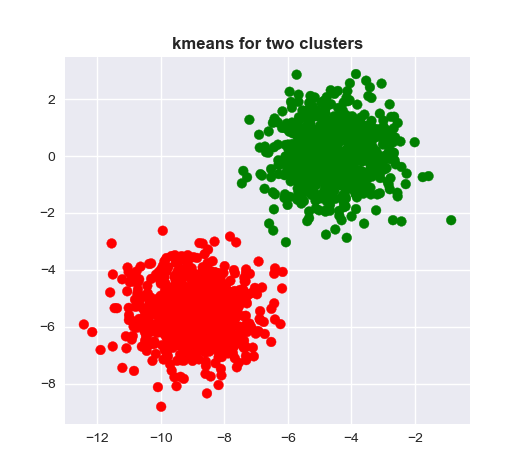
\includegraphics[width=0.5\linewidth]{../figures/statisticalLearning/unsupervisedLearning/kmeansExample}
\caption{Demonstration of k-means clustering on a data set with two blobs. Code: kmeansExample.py}
\label{fig:kmeansExample}
\end{figure}


\subsubsection{K means ++}

k means ++ 

\subsubsection{Kernel K means}

\href{https://sites.google.com/site/dataclusteringalgorithms/kernel-k-means-clustering-algorithm}{link}

\subsection{Gaussian mixture models}

\begin{definition}[Gaussian mixture model problems]\index{Gaussian mixture model}
Given a set of points $x_1,...,x_T \in \R^D$, the goal is to find a data generation model 
$$p(x|\theta) = \sum_{i=1}^M w_i g_i(x|\mu_i,\Sigma_i),$$ where the mixture weights satisfying $\sum_{i=1}^M w_i = 1$,
parameterized by $\theta=\{w_i,\mu_i, \Sigma_i,i=1,...,M\},$ given as 

	$$g(x|\mu_i,\Sigma_i) = \frac{1}{(2\pi)^{D/2}\abs{ \Sigma_i}^{1/2}}\exp(-(x-\mu_i)^T\Sigma_i^{-1}(x-\mu_i))$$

such that likelihood for the observed data
$$L = \prod_{i=1}^T p(x_i|\theta)$$
is maximized.
\end{definition}


\begin{algorithm}[H]
	\SetAlgoLined
	\KwIn{Data set consists of $x_1,x_2,...,x_N$}
	Set $n=0$, and set initial values $\lambda$.\\
	
	M step: 
	$$Pr(i|x_t,\lambda)=\frac{w_i g(x_t|\mu_t,\Sigma_t)}{\sum_{k=1}^M w_k g_i(x_k|\mu_k, \Sigma_k)},\forall i\in\{1,...,M\}, \forall t\in \{1,...,T\}$$
	
	
	E step: update $\lambda$ as

	$$w_i = \frac{1}{T} \sum_{i=t}^T Pr(i|x_t,\lambda),\forall i$$
	
	$$\mu_i = \frac{\sum_{t=1}^T Pr(i|x_t,\lambda) x_i}{\sum_{t=1}^T Pr(i|x_t,\lambda)},\forall i$$
	
	
	$$\sigma_i^2 = \frac{\sum_{t=1}^T Pr(i|x_t,\lambda) x_t^2}{\sum_{t=1}^T Pr(i|x_t,\lambda)} - \mu_i^2,\forall i$$
	
	
	\KwOut{the optimalized value $\theta$.}
	\caption{Gaussian mixture model EM algorithm}
\end{algorithm}

\begin{remark}[applications]
GMMs have been used recently for feature extraction from speech data for use in speech recognition systems[4]. They have also been used extensively in object tracking of multiple objects, where the number of mixture components and their means predict object locations at each frame in a video sequence[5]. The EM algorithm is used to update the component means over time as the video frames update, allowing object tracking.	
\end{remark}


\subsection{Spectral clustering}


\begin{algorithm}[H]
	\SetAlgoLined
	\KwIn{Data set consists of $x_1,x_2,...,x_N$}
	Construct a similarity graph. Let $W$ be the weighted adjacency matrix.\\
	Compute a Laplacian $L$ or $(L_{sys},L_{rw})$.\\
	Compute the first top $k$ eigenvectors $u_1,..,u_k \in \R^N$ of $L$.\\
	Assign each data point $i$ with the new lower dimensional coordinate $y_i = (u_{1,i},u_{2,i},...,u_{k,i})$.\\
	Use $K$-means algorithms to do clustering on the lower dimensional coordinates.
	
	\KwOut{clustered results}
	\caption{General spectral clustering algorithm}
\end{algorithm}

\begin{remark}[We do not ignore eigenvectors associated with zero eigenvalue]\hfill
\begin{itemize}
	\item Note that in diffusion mapping and Laplacian eigenmap, we will ignore the top eigenvector, because the top eigenvector (the multiplicity is  1 usually)is constant 1 vector that does not provide extra information.
	\item In spectral clustering, the eigenvector associated with zero eigenvalues(the multiplicity is greater than 1 usually) will provide information on distance.
\end{itemize}
\end{remark}



\begin{remark}[which Laplacian to use?\cite{von2007tutorial}]\hfill
\begin{itemize}
	\item If the graph is very regular and most vertices have approximately the same degree, then all Laplacians are very similar to each other.
	\item If the graph is not regular, then use $L_{rw}$. 
\end{itemize}
\end{remark}






\section{Notes on Bibliography}
Excellent treatment on PCA and its generalization, see \cite{vidal2016generalized}.

For machine learning theory, see \cite{mitchell1997machine}.
For multidimensional scaling, see\cite{borg2005modern}.
For spectral clustering, see \cite{von2007tutorial}.
For ensemble methods, see \cite{zhou2012ensemble}.
For boosting, see \cite{schapire2012boosting}.

\printbibliography
\end{refsection}
